\documentclass{article}
\usepackage[margin=1in]{geometry}
\usepackage{graphicx}
\usepackage{float}
\usepackage{caption}
\usepackage[UTF-8]{ctex}
\usepackage{multirow}
\usepackage{booktabs}
\usepackage{ulem}

\begin{document}

\begin{center}
    \LARGE\textbf{Recent Results of Reappearance Experiment} \\[0.5cm]
    \large Haruko386 | 2025 年 6 月 10 日 \\
\end{center}

\section{Marigold}

本周我主要的工作就是对\textit{\textbf{Marigold}}的结果进行二次复现。之前的复现仅仅使用了\textit{Vkitti}数据集;\textit{Vkitti}数据集的主要内容为路面上的行车路况,
数据集丰富度较差,因此只适合作为补充内容。现在配置好\textit{Hypersim}数据集后,重新训练了\textit{\textbf{Marigold}}模型,模型在各数据集上的评估如下表。

\begin{table*}[ht]
\centering
\small
\resizebox{\textwidth}{!}{
\begin{tabular}{lcccccccccccccc}
\toprule
\multirow{2}{*}{\textbf{Method}} & \multicolumn{2}{c}{\textbf{\# Training samples}} & \multicolumn{2}{c}{\textbf{NYUv2}} & \multicolumn{2}{c}{\textbf{KITTI}} & \multicolumn{2}{c}{\textbf{ETH3D}} & \multicolumn{2}{c}{\textbf{ScanNet}} & \multicolumn{2}{c}{\textbf{DIODE}} & \multirow{2}{*}{\textbf{Avg.}} \\
 & Real & Synthetic & AbsRel↓ & δ1↑ & AbsRel↓ & δ1↑ & AbsRel↓ & δ1↑ & AbsRel↓ & δ1↑ & AbsRel↓ & δ1↑ & Rank \\
\midrule
DiverseDepth [56] & 320K & --- & 11.7 & 87.5 & 19.0 & 70.4 & 22.8 & 69.4 & 10.9 & 88.2 & 37.6 & 63.1 & 7.6 \\
MiDaS [35] & 2M & --- & 11.1 & 88.5 & 23.6 & 63.0 & 18.4 & 75.2 & 12.1 & 84.6 & 33.2 & 71.5 & 7.3 \\
LeReS [57] & 300K & 54K & 9.0 & 91.6 & 14.9 & 78.4 & 17.1 & 77.7 & 9.1 & 91.7 & 27.1 & 76.6 & 5.2 \\
Omnidata [13] & 11.9M & 310K & 7.4 & 94.5 & 14.9 & 83.5 & 16.6 & 77.8 & 7.5 & 93.6 & 33.9 & 74.2 & 4.8 \\
HDN [60] & 300K & --- & 6.9 & 94.8 & 11.5 & 86.7 & 12.1 & 83.3 & 8.0 & 93.9 & 24.6 & \textbf{78.0} & 3.2 \\
DPT [36] & 1.2M & 188K & 9.8 & 90.3 & 10.0 & 90.1 & 7.8 & 94.6 & 8.2 & 93.4 & \textbf{18.2} & 75.8 & 3.9 \\
\midrule
Ours (w/o ensemble) & --- & 74K & 6.0 & 95.9 & 10.5 & 91.6 & 7.1 & 95.1 & 6.9 & 94.5 & 31.0 & 77.2 & 2.5 \\
Ours (w/ ensemble) & --- & 74K & \textbf{5.5} & \textbf{96.4} & \textbf{9.9} & \textbf{91.6} & \textbf{6.5} & \textbf{96.0} & \textbf{6.4} & \textbf{95.1} & 30.8 & 77.3 & \textbf{1.4} \\
\textbf{Trained (extra)} & --- & 75.5K & & & & & & & & & & & \\
\bottomrule
\end{tabular}
}
\caption{在不同数据集上,不同模型的测试结果。}
\end{table*}


本次复现,我使用了74K的训练样本(\textit{\textbf{Hypersim}}: 68.5GB + \textit{\textbf{Vkitti}}: 7GB),在单张RTX 4090上一共训练21000轮次,
大约60小时训练时长。从表中数据对比可以看出,在添加了具有更多场景的\textit{Hypersim}数据集后,复现的结果已经相当接近原论文。

\begin{figure}[H]
  \centering
  \small % 缩小字号
  \setlength{\tabcolsep}{2pt} % 减少列间距,增加紧凑度
  \begin{tabular}{cccccc}
    \textbf{Input} & \textbf{Vkitti only} & \textbf{Marigold} & \textbf{Input} & \textbf{Vkitti only} & \textbf{Marigold} \\
    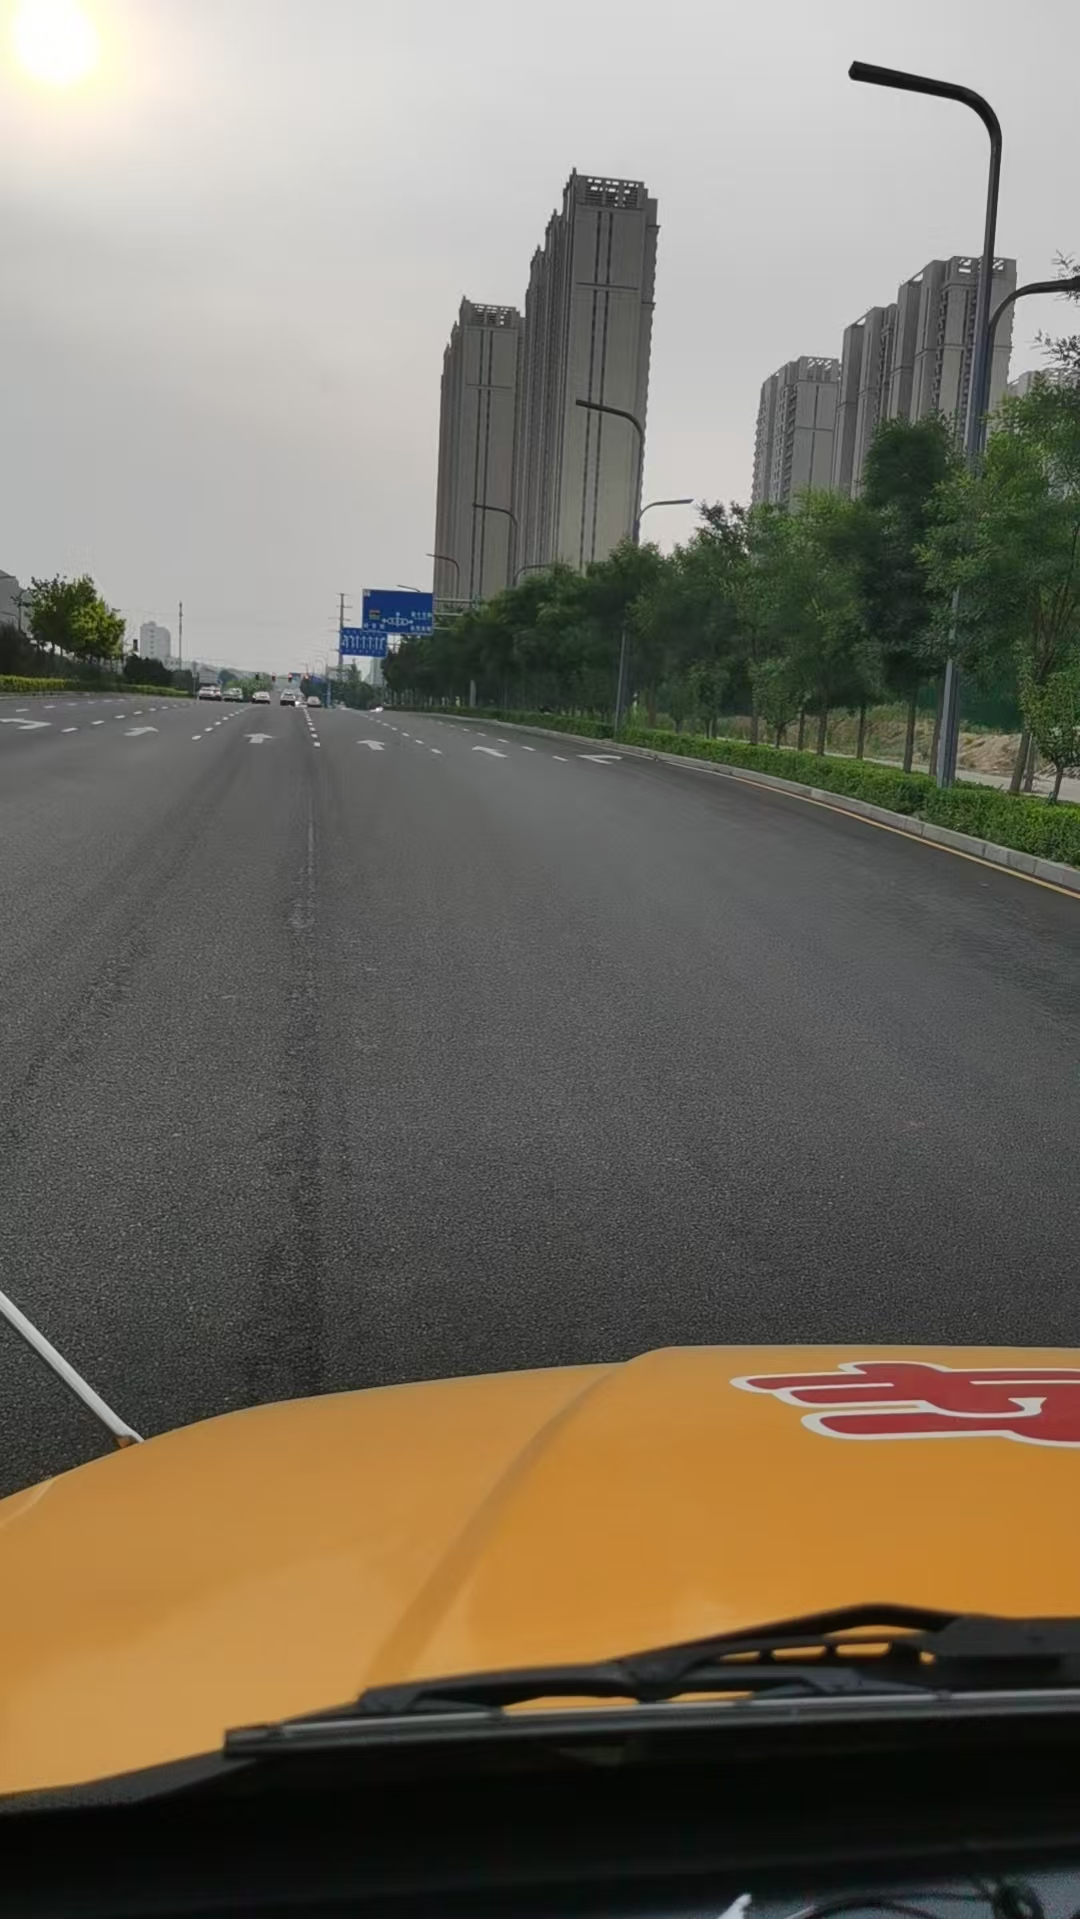
\includegraphics[width=0.15\textwidth,height=3.5cm,keepaspectratio]{images/on-the-road/1.jpg} &
    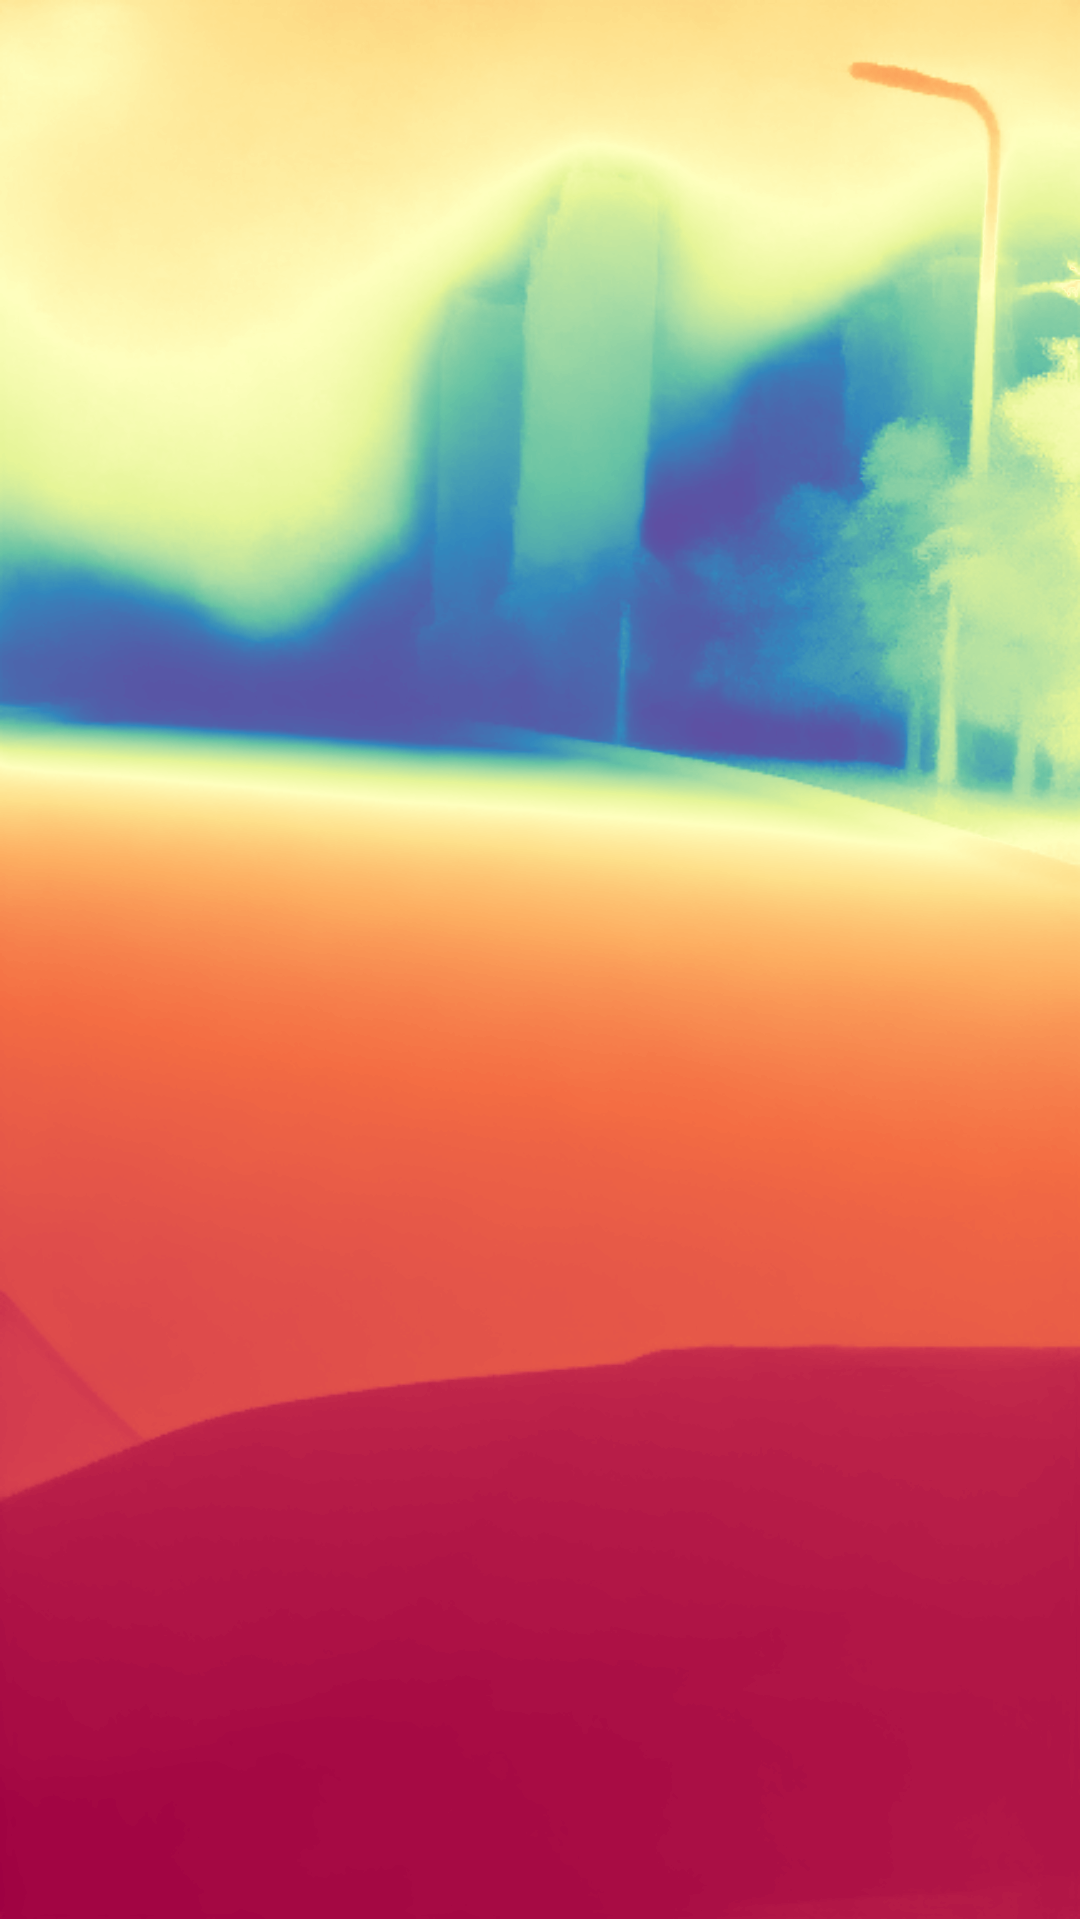
\includegraphics[width=0.15\textwidth,height=3.5cm,keepaspectratio]{images/real_image_trained/depth_colored/1.png} &
    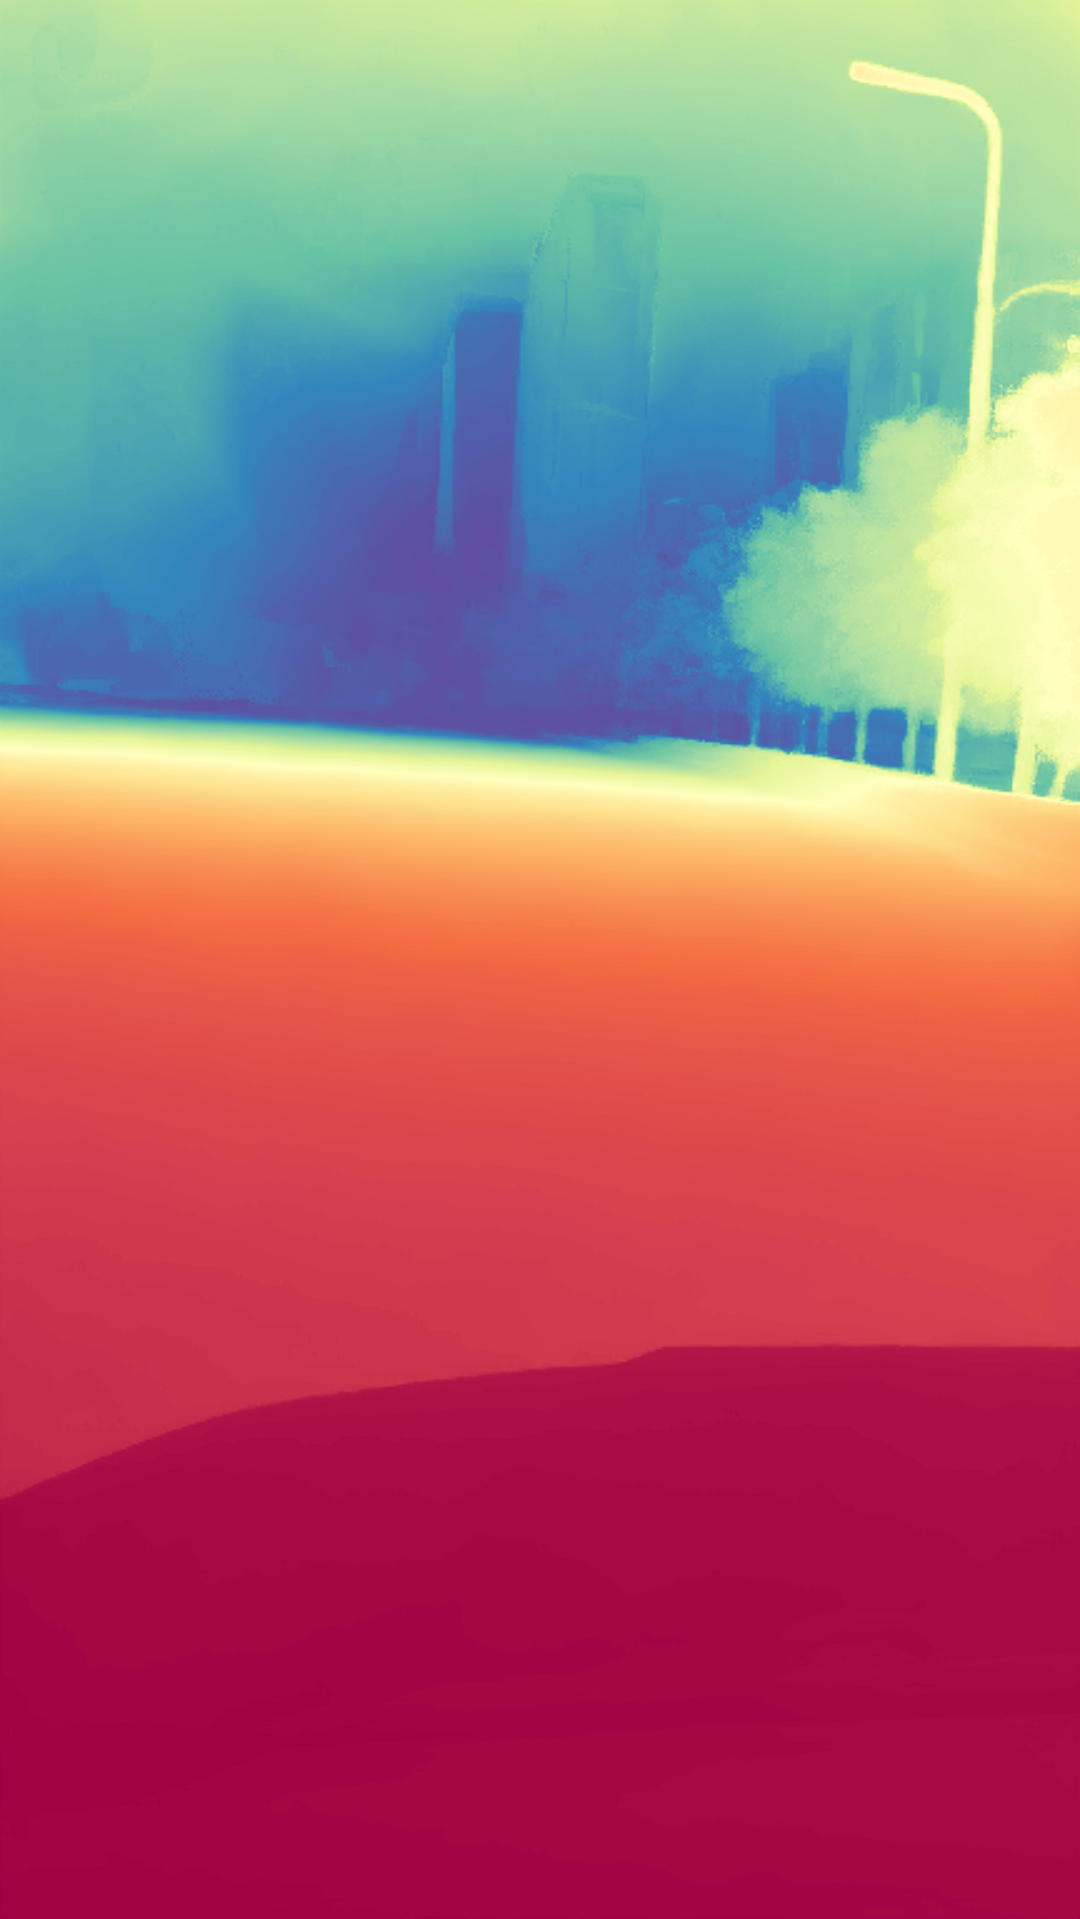
\includegraphics[width=0.15\textwidth,height=3.5cm,keepaspectratio]{images/real_image/depth_colored/1.png} &
    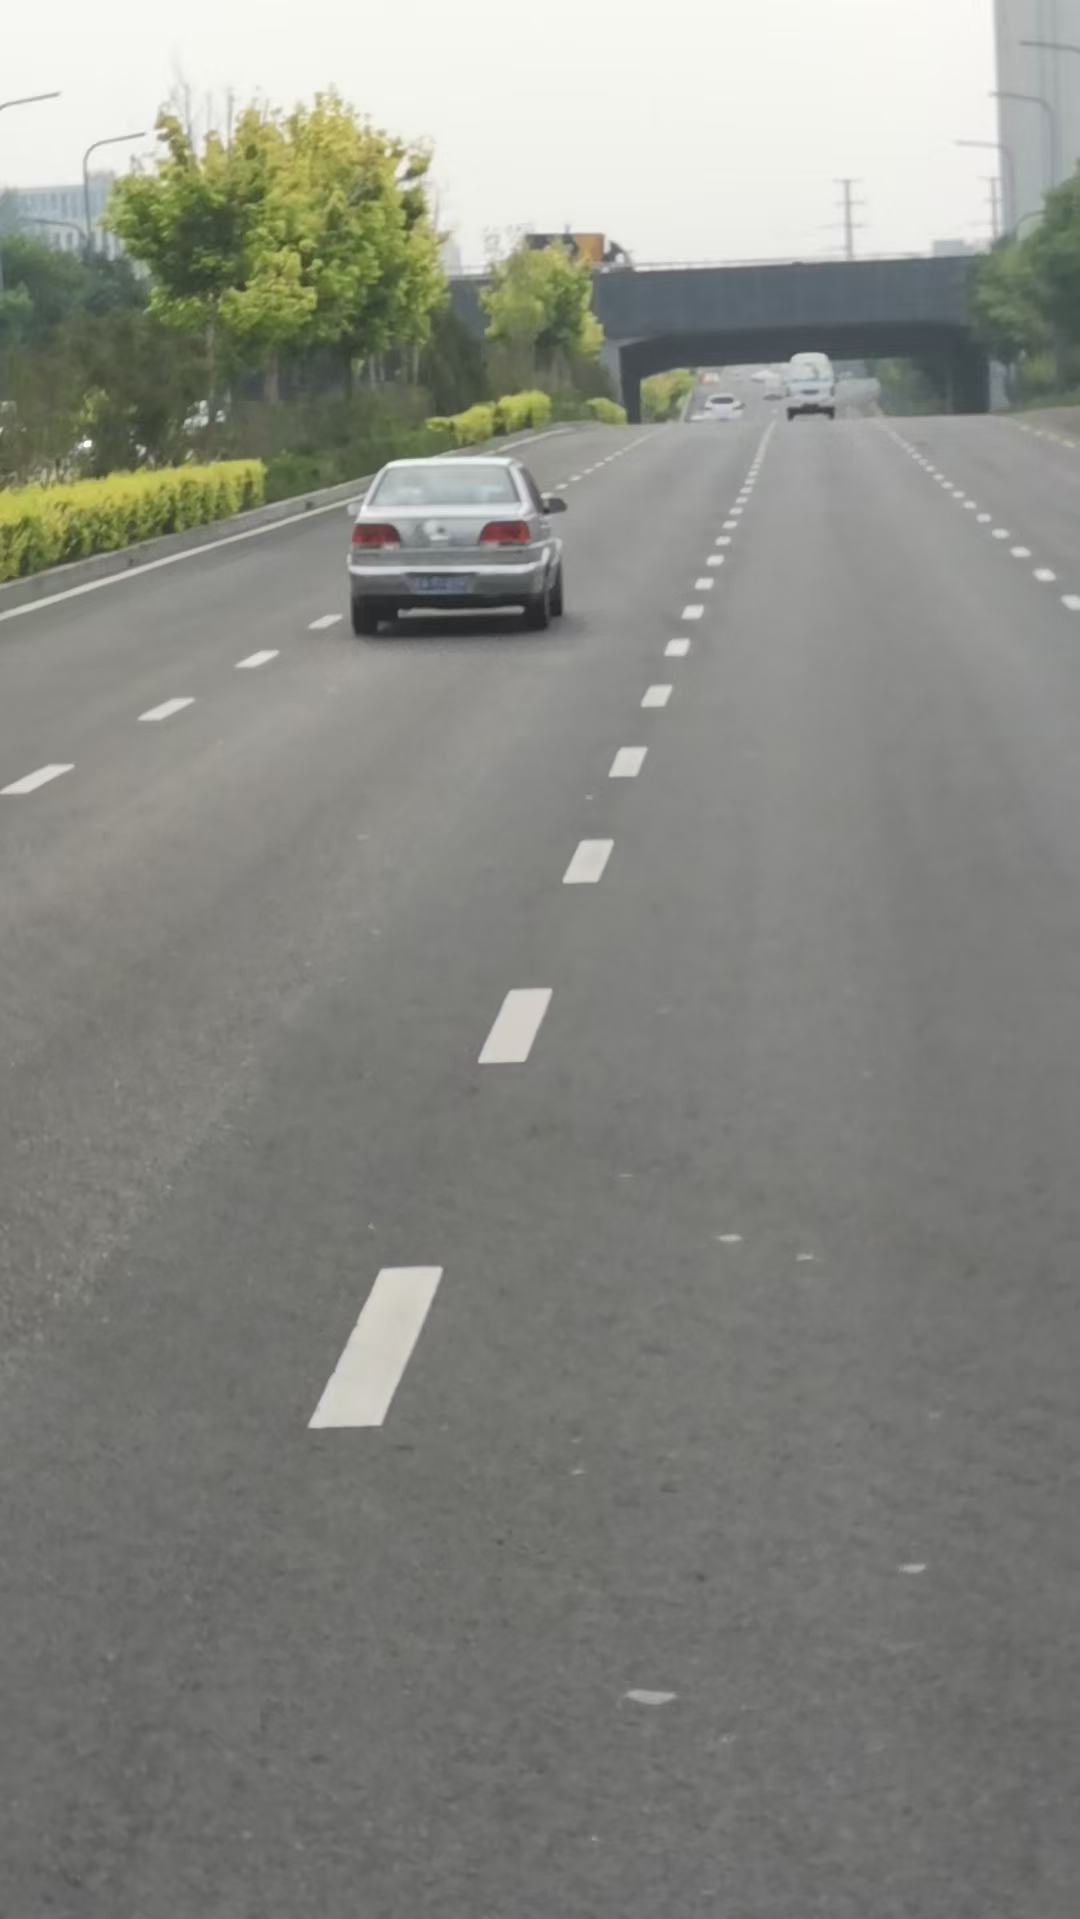
\includegraphics[width=0.15\textwidth,height=3.5cm,keepaspectratio]{images/on-the-road/2.jpg} &
    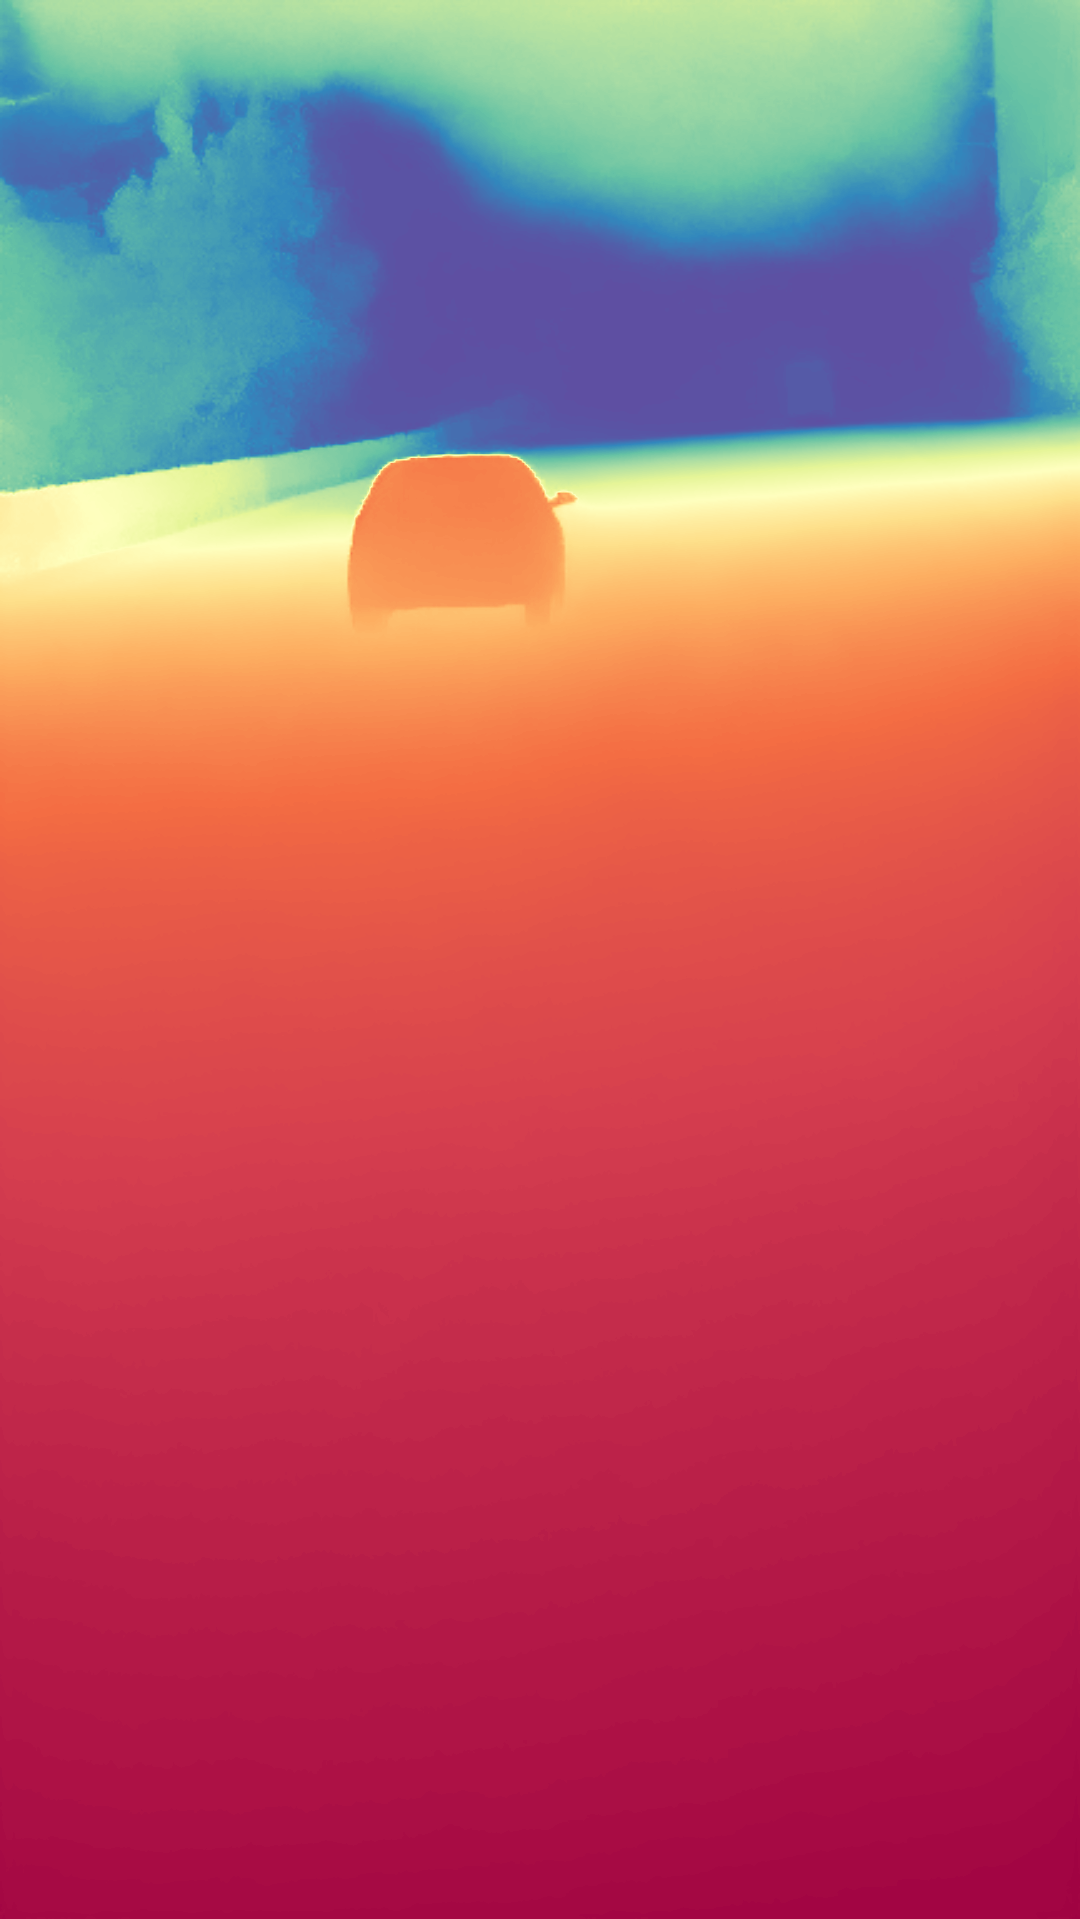
\includegraphics[width=0.15\textwidth,height=3.5cm,keepaspectratio]{images/real_image_trained/depth_colored/2.png} &
    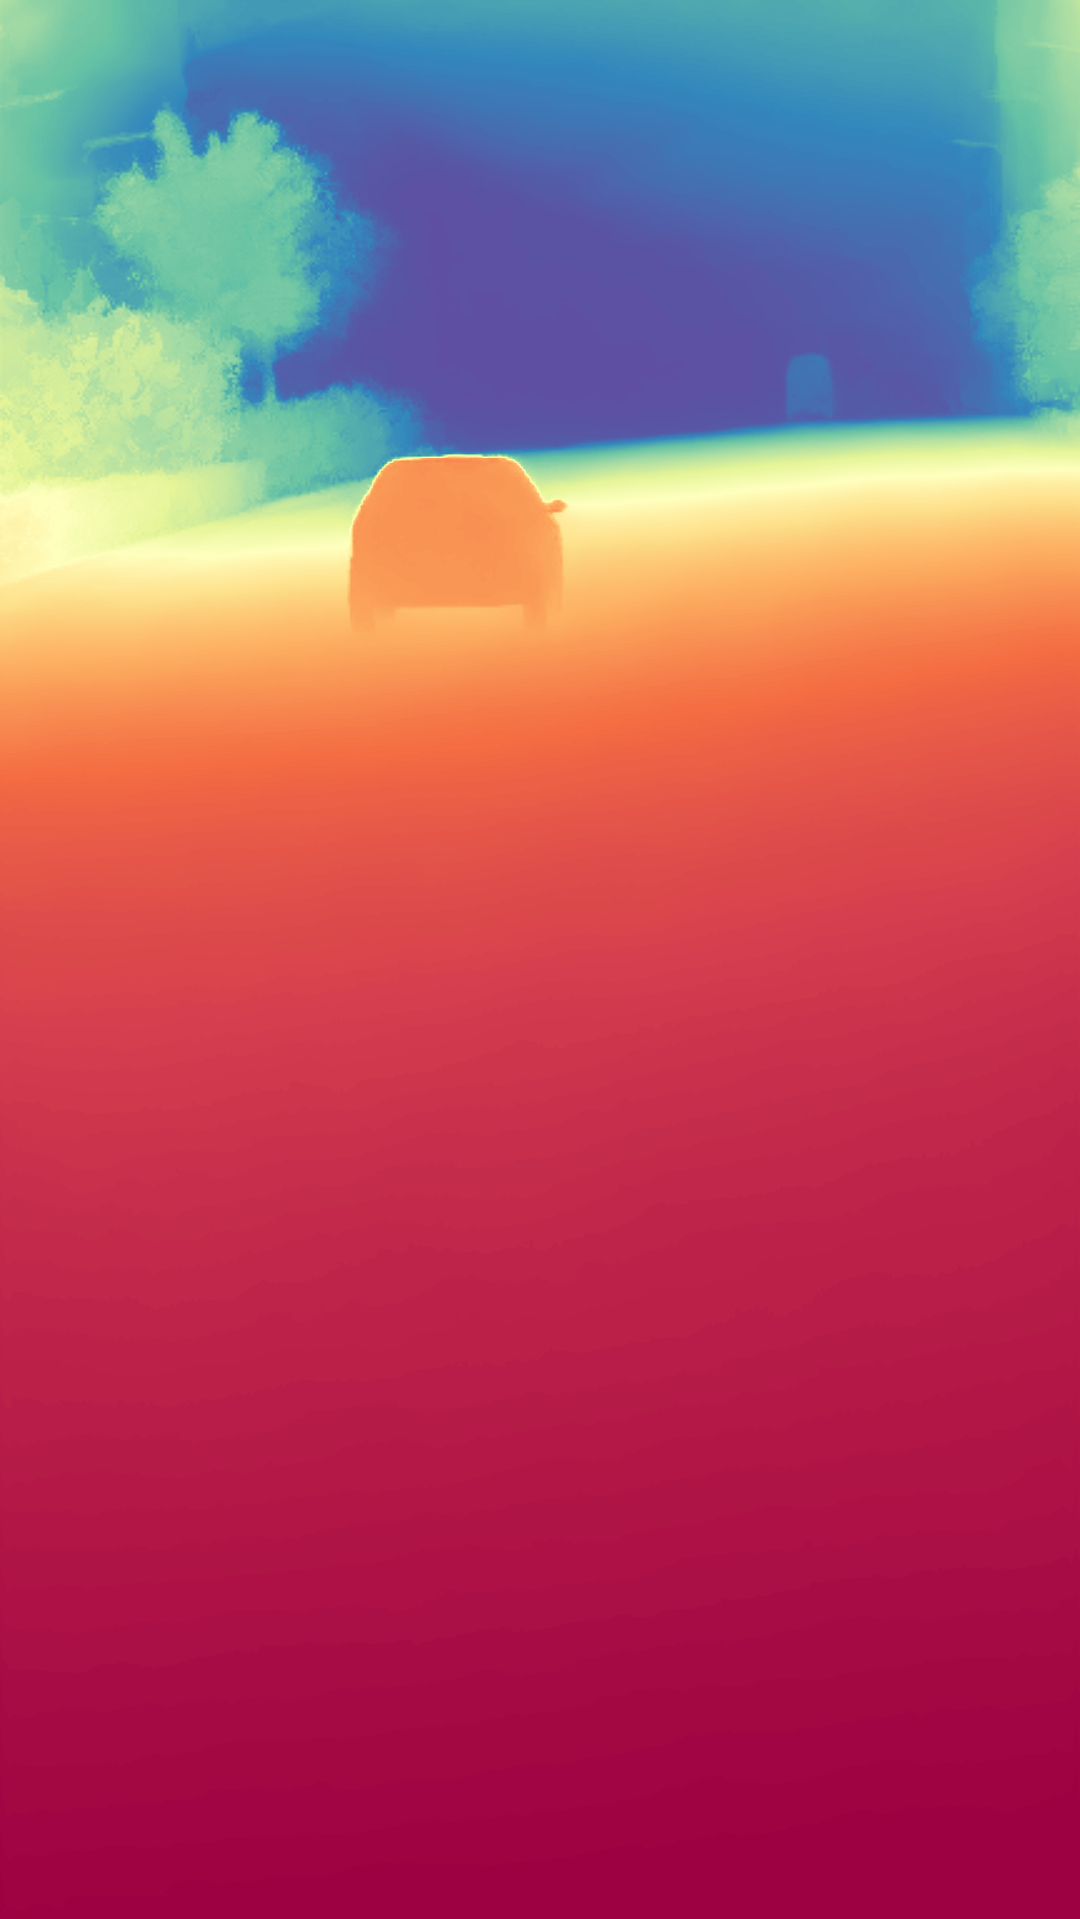
\includegraphics[width=0.15\textwidth,height=3.5cm,keepaspectratio]{images/real_image/depth_colored/2.png} \\
  \end{tabular}
  \begin{tabular}{cccccc}
    \textbf{Input} & \textbf{Vkitti only} & \textbf{Marigold} & \textbf{Input} & \textbf{Vkitti only} & \textbf{Marigold} \\
    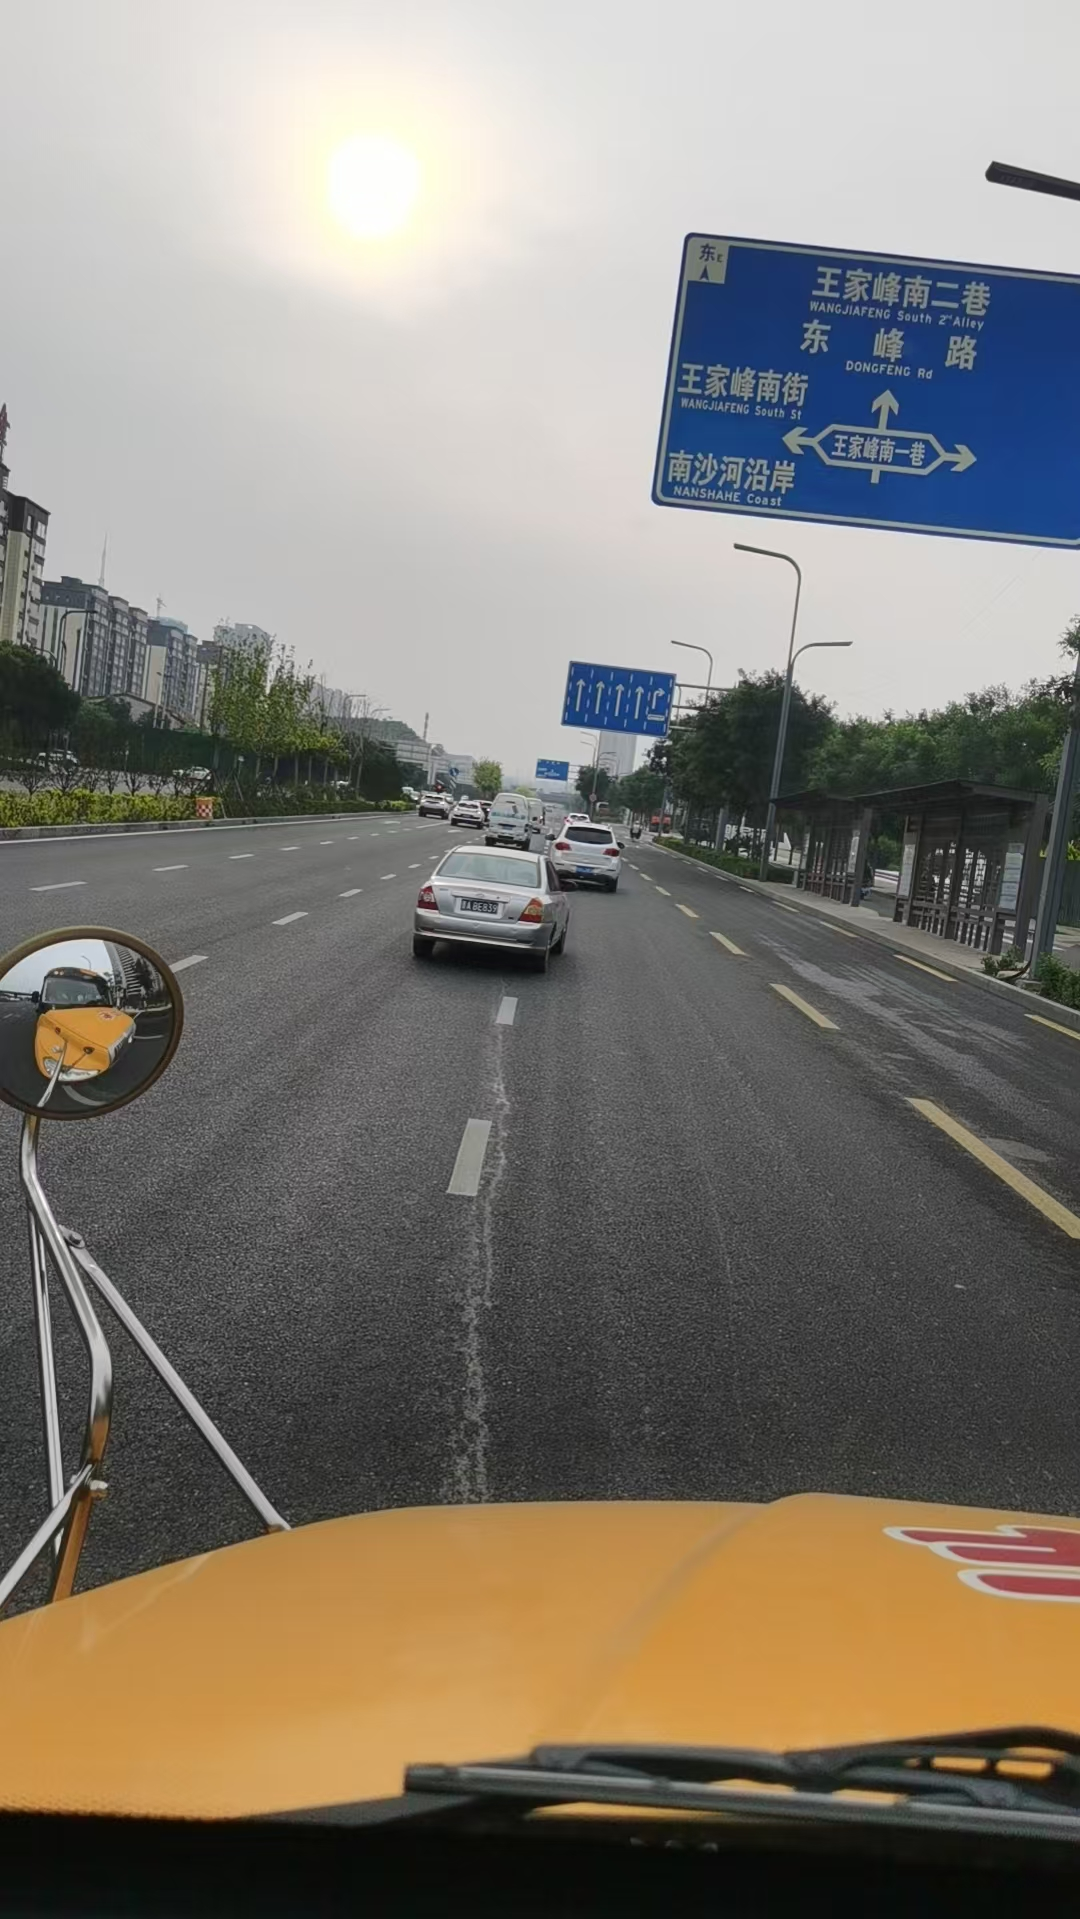
\includegraphics[width=0.15\textwidth,height=3.5cm,keepaspectratio]{images/on-the-road/3.jpg} &
    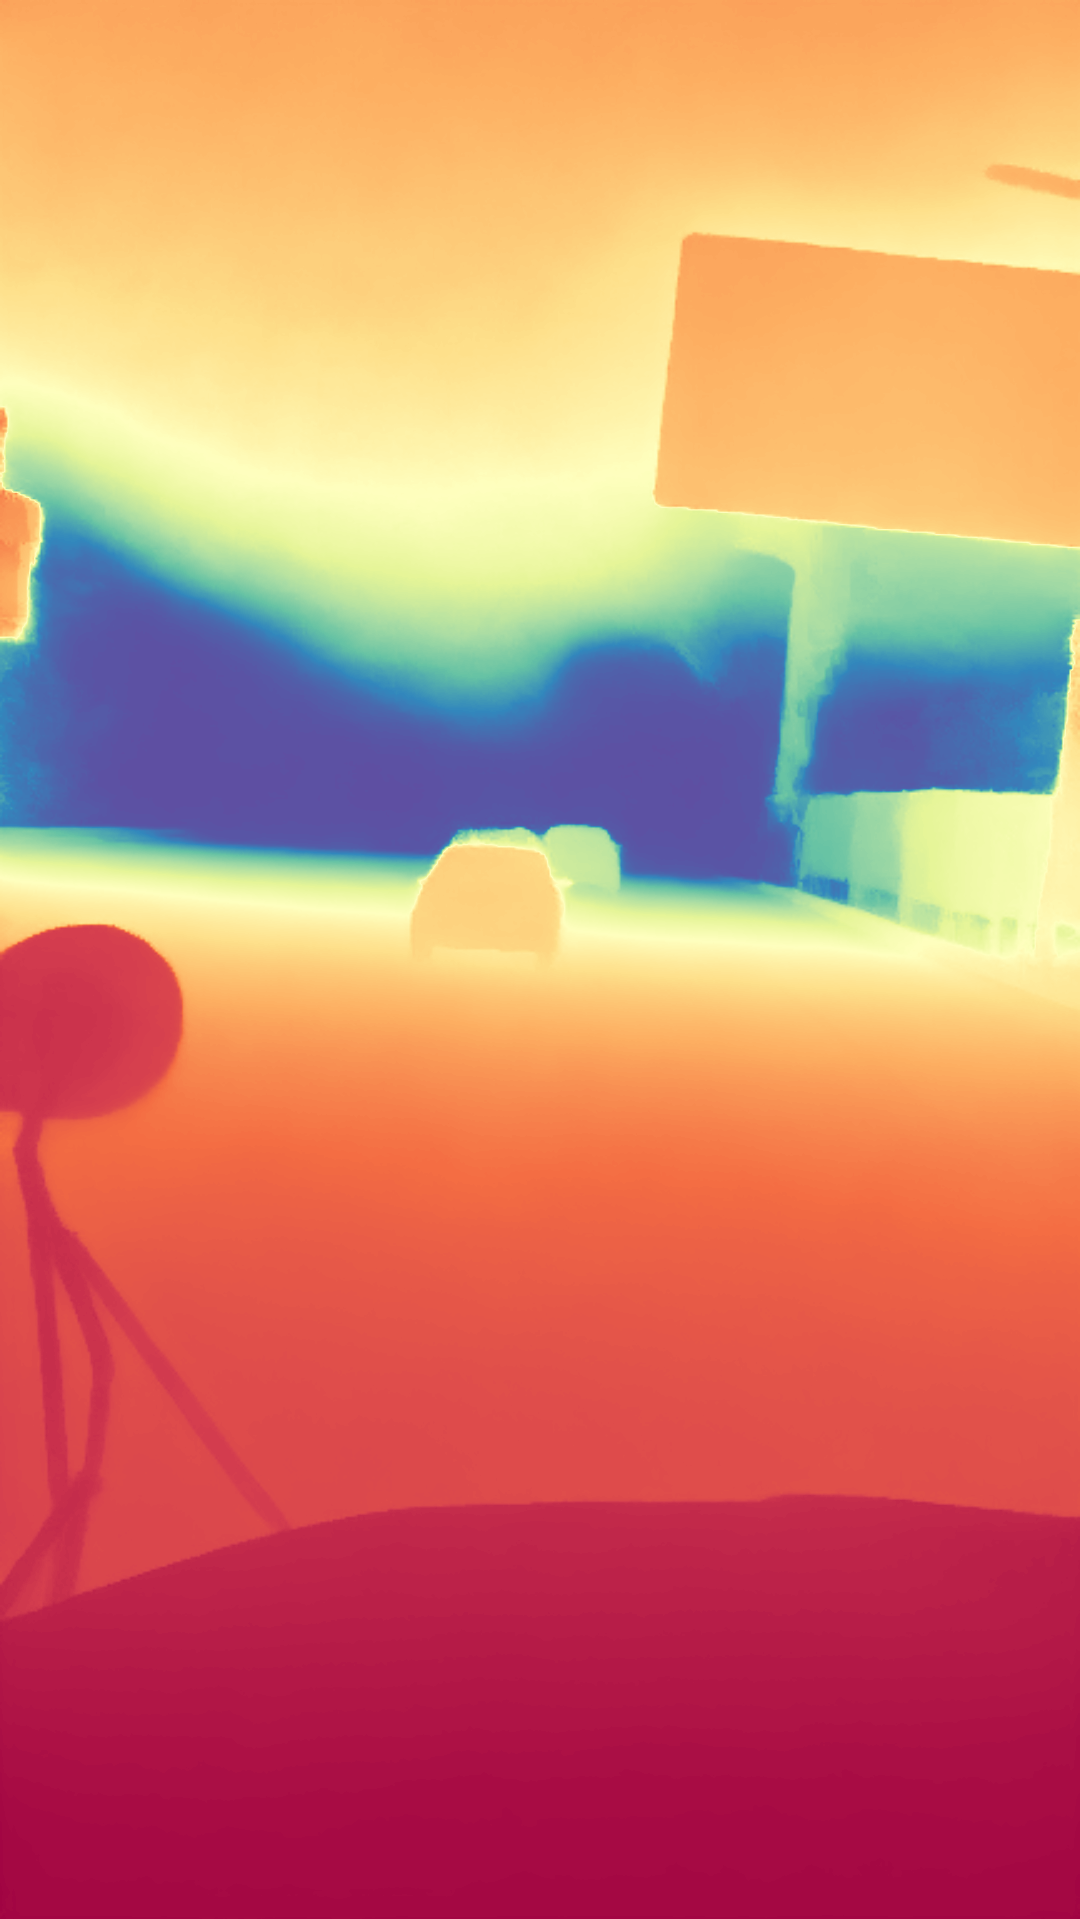
\includegraphics[width=0.15\textwidth,height=3.5cm,keepaspectratio]{images/real_image_trained/depth_colored/3.png} &
    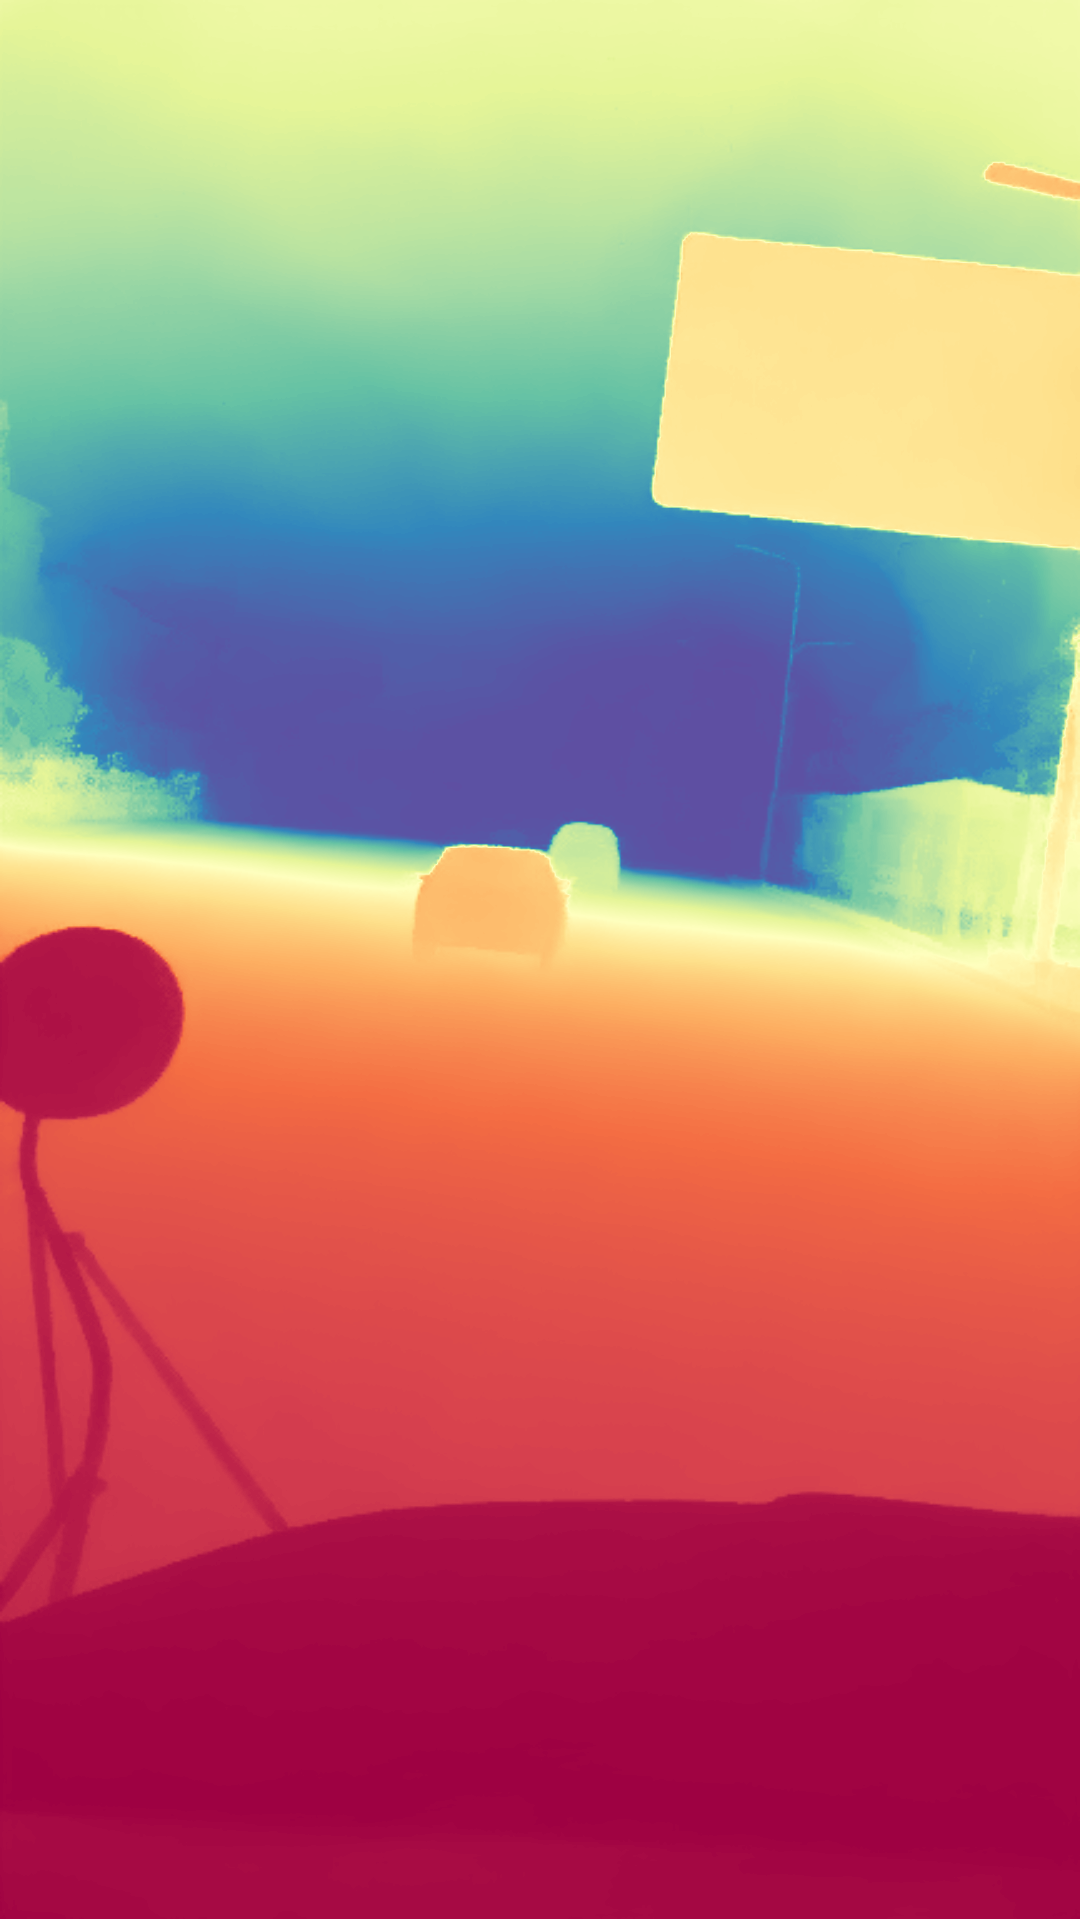
\includegraphics[width=0.15\textwidth,height=3.5cm,keepaspectratio]{images/real_image/depth_colored/3.png} &
    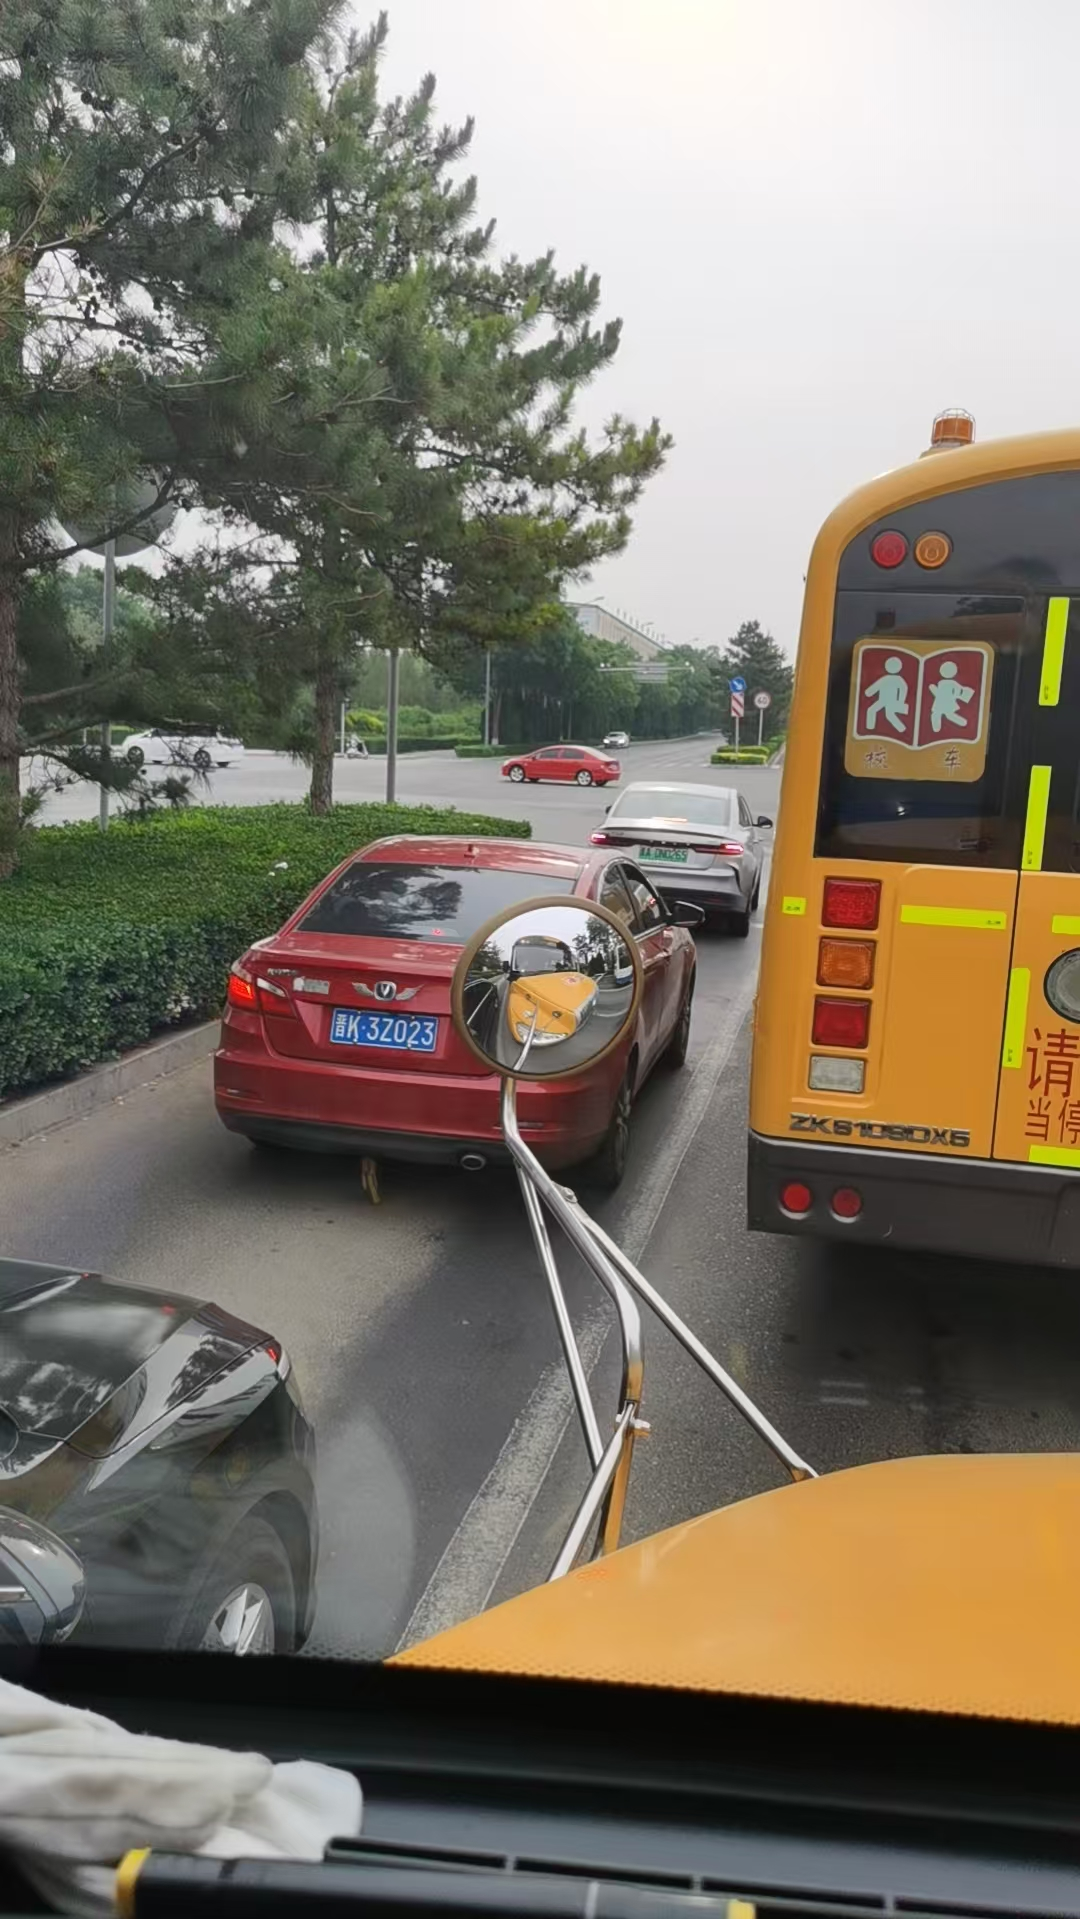
\includegraphics[width=0.15\textwidth,height=3.5cm,keepaspectratio]{images/on-the-road/4.jpg} &
    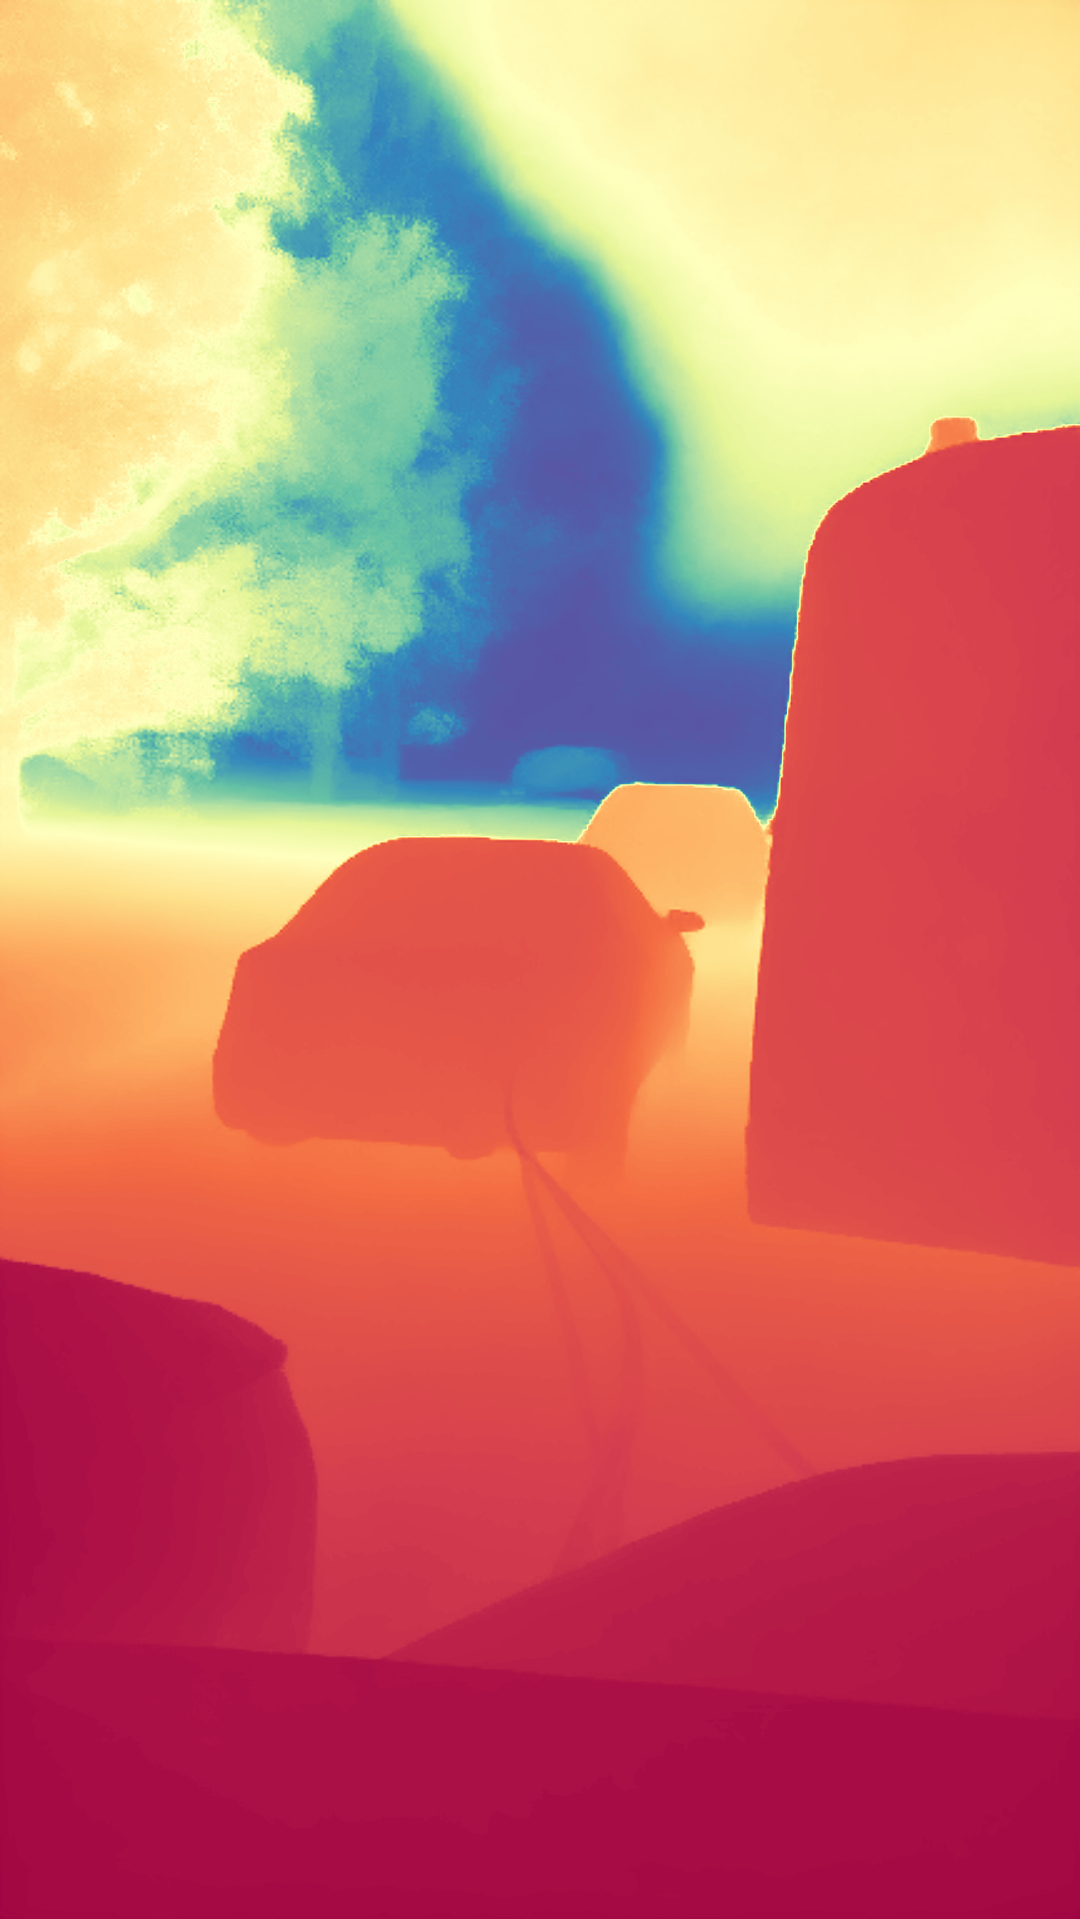
\includegraphics[width=0.15\textwidth,height=3.5cm,keepaspectratio]{images/real_image_trained/depth_colored/4.png} &
    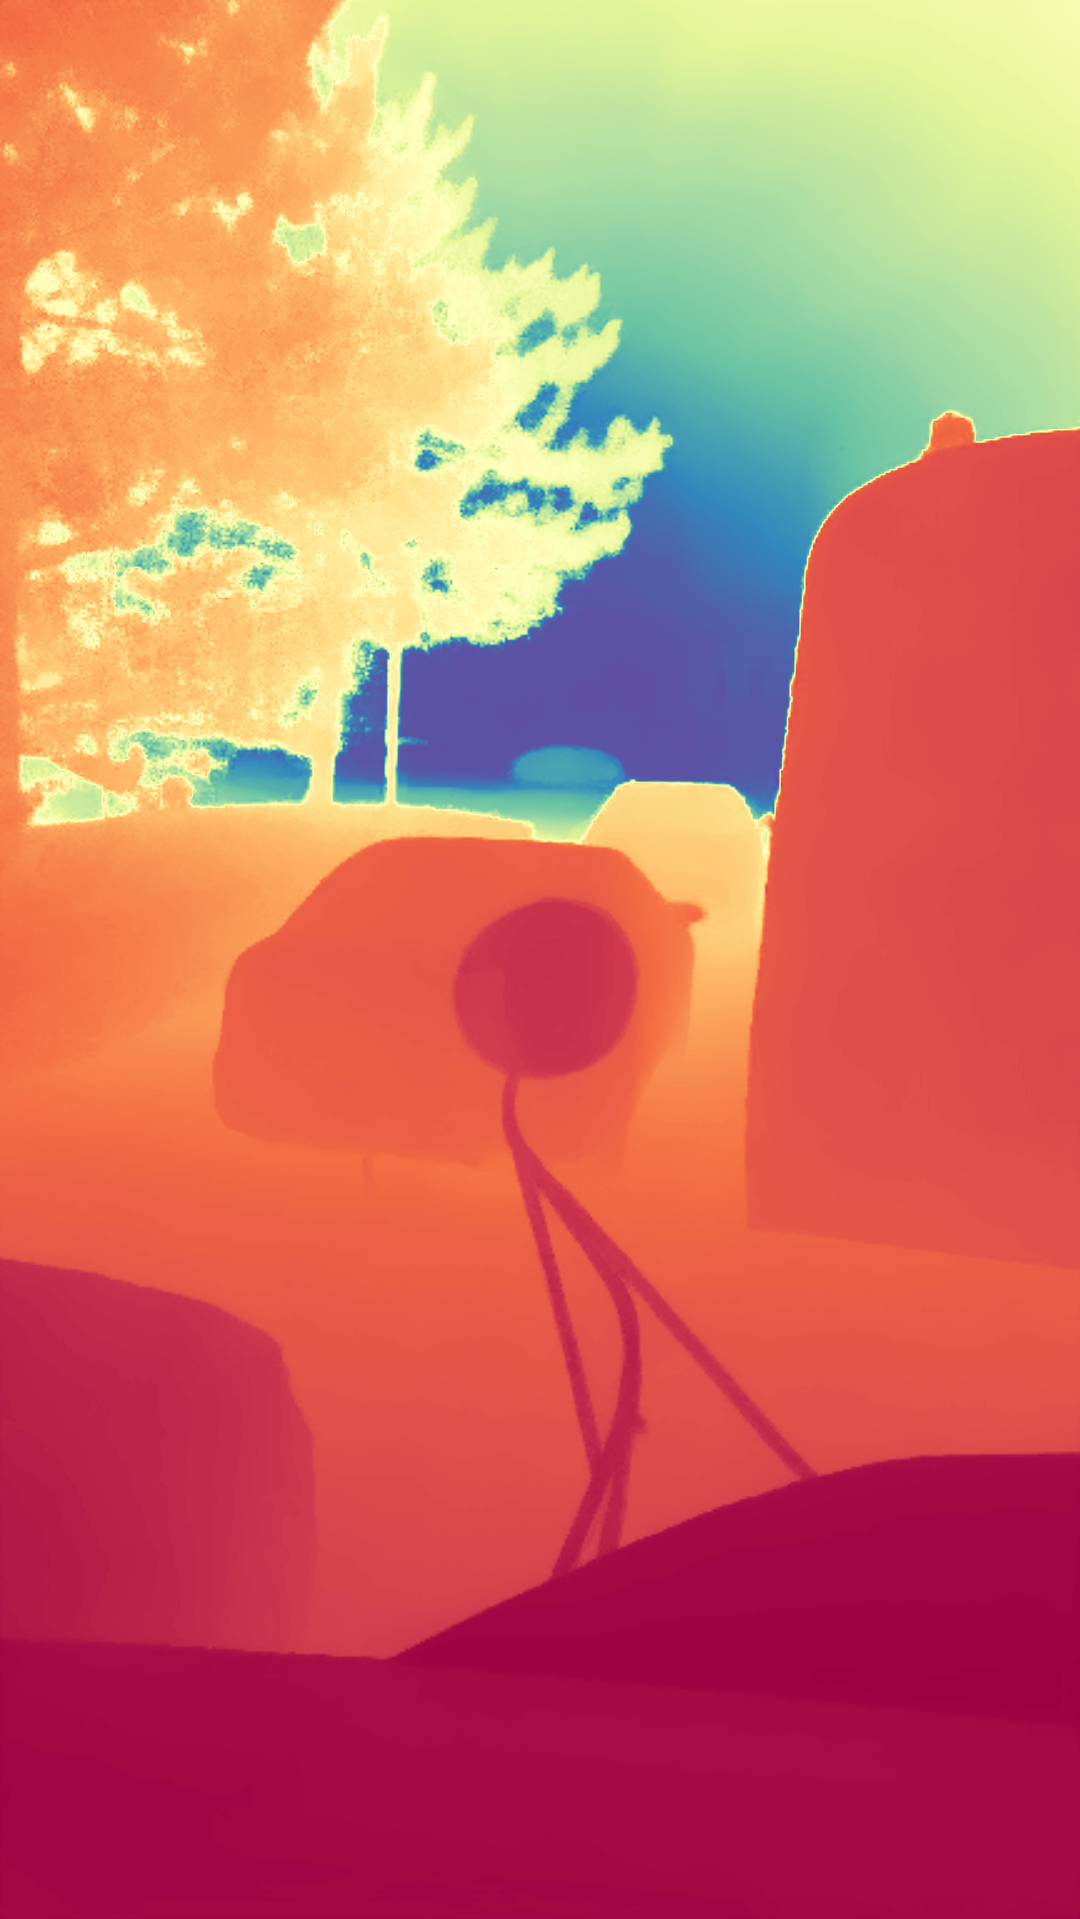
\includegraphics[width=0.15\textwidth,height=3.5cm,keepaspectratio]{images/real_image/depth_colored/4.png} \\
  \end{tabular}
  \caption{仅在\textit{Vkitti}数据集上训练的模型在实际道路图像上的表现}
\end{figure}

\begin{figure}[H]
  \centering
  \begin{tabular}{cccc}
    \textbf{Input RGB Image} & \textbf{Trained iter: 3450} & \textbf{Marigold} & \textbf{DepthMaster} \\
    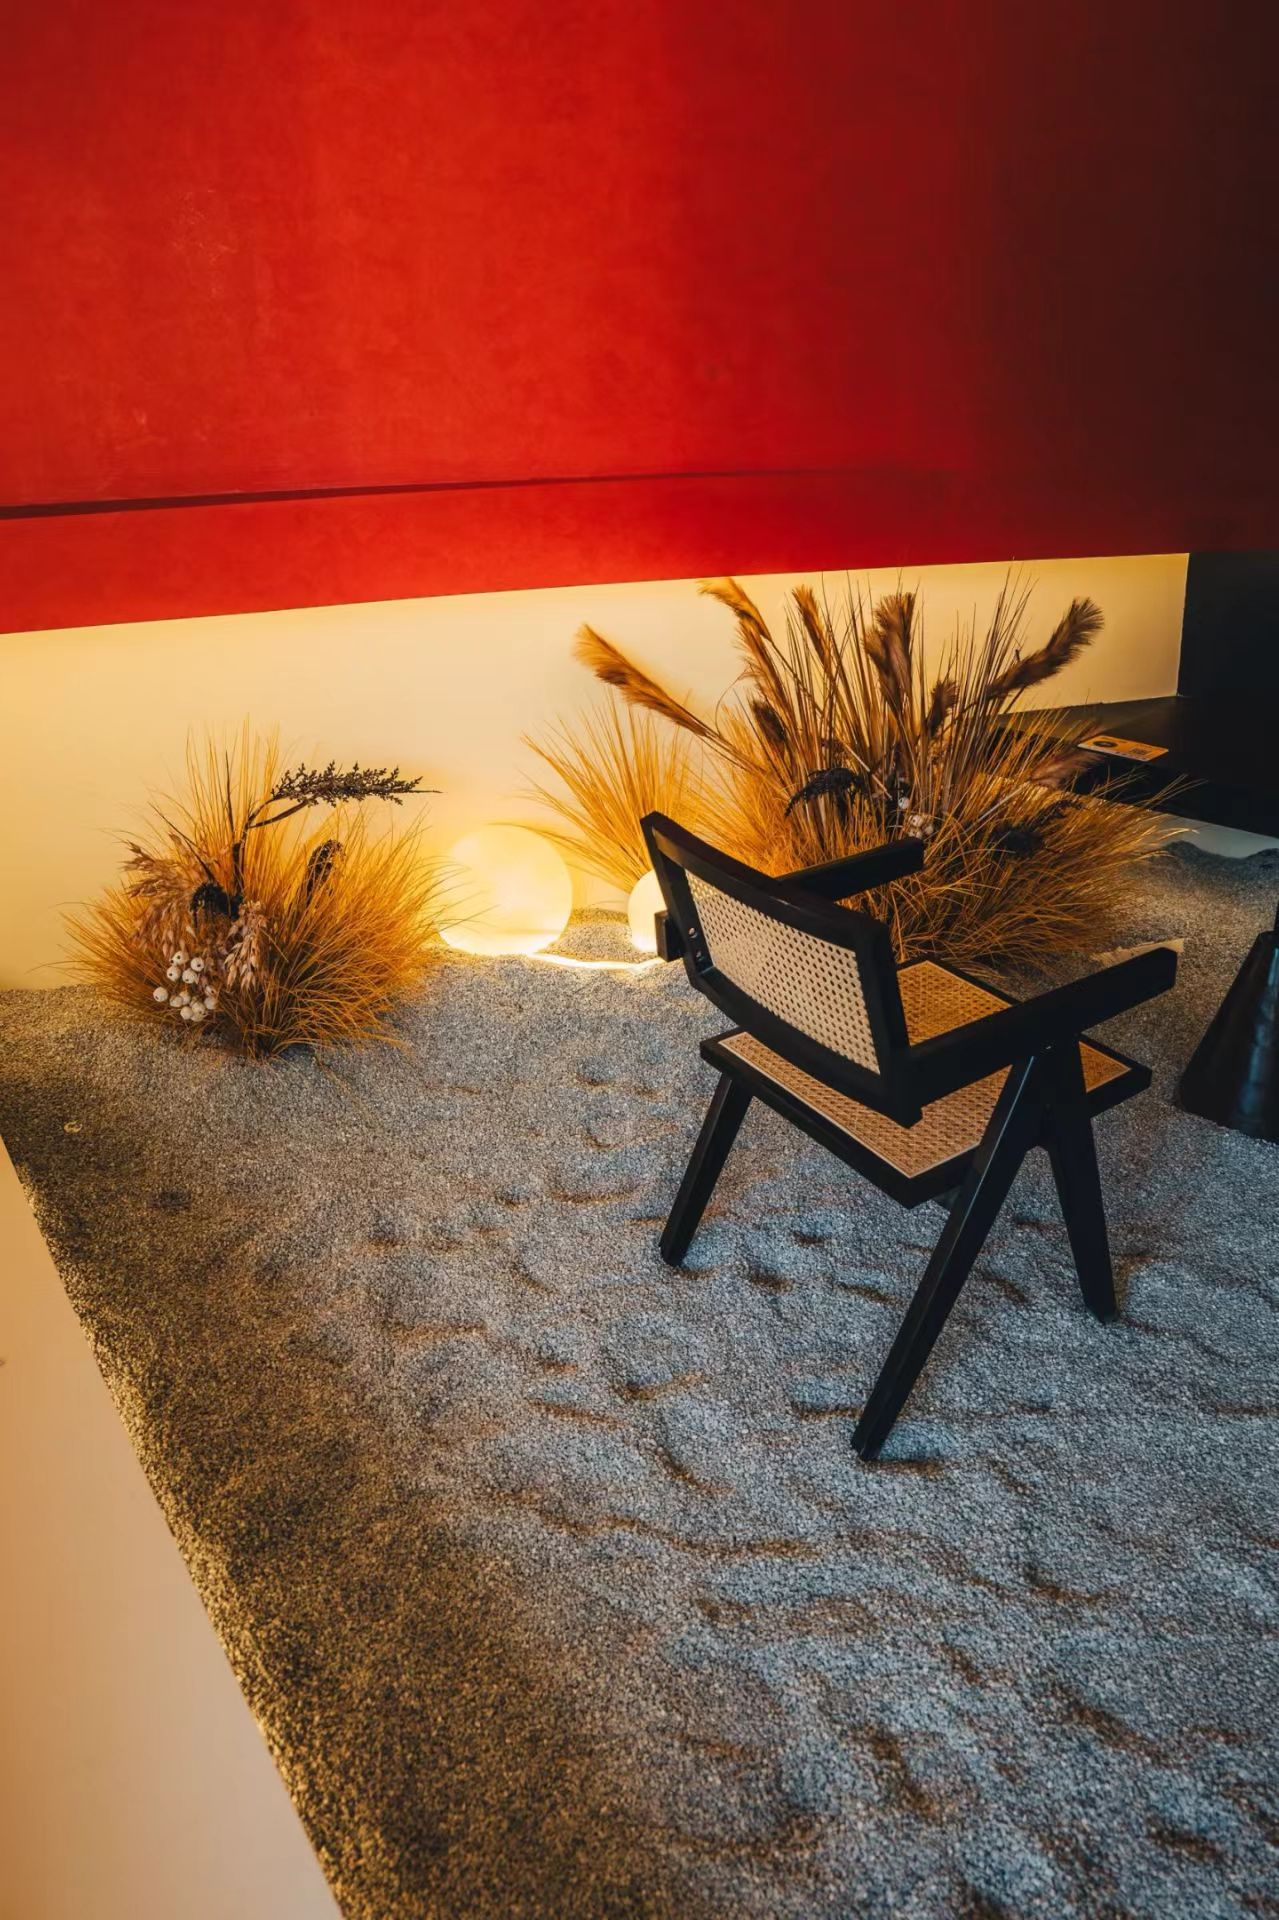
\includegraphics[width=0.2\textwidth]{images/test-image/inside-02.jpg} &
    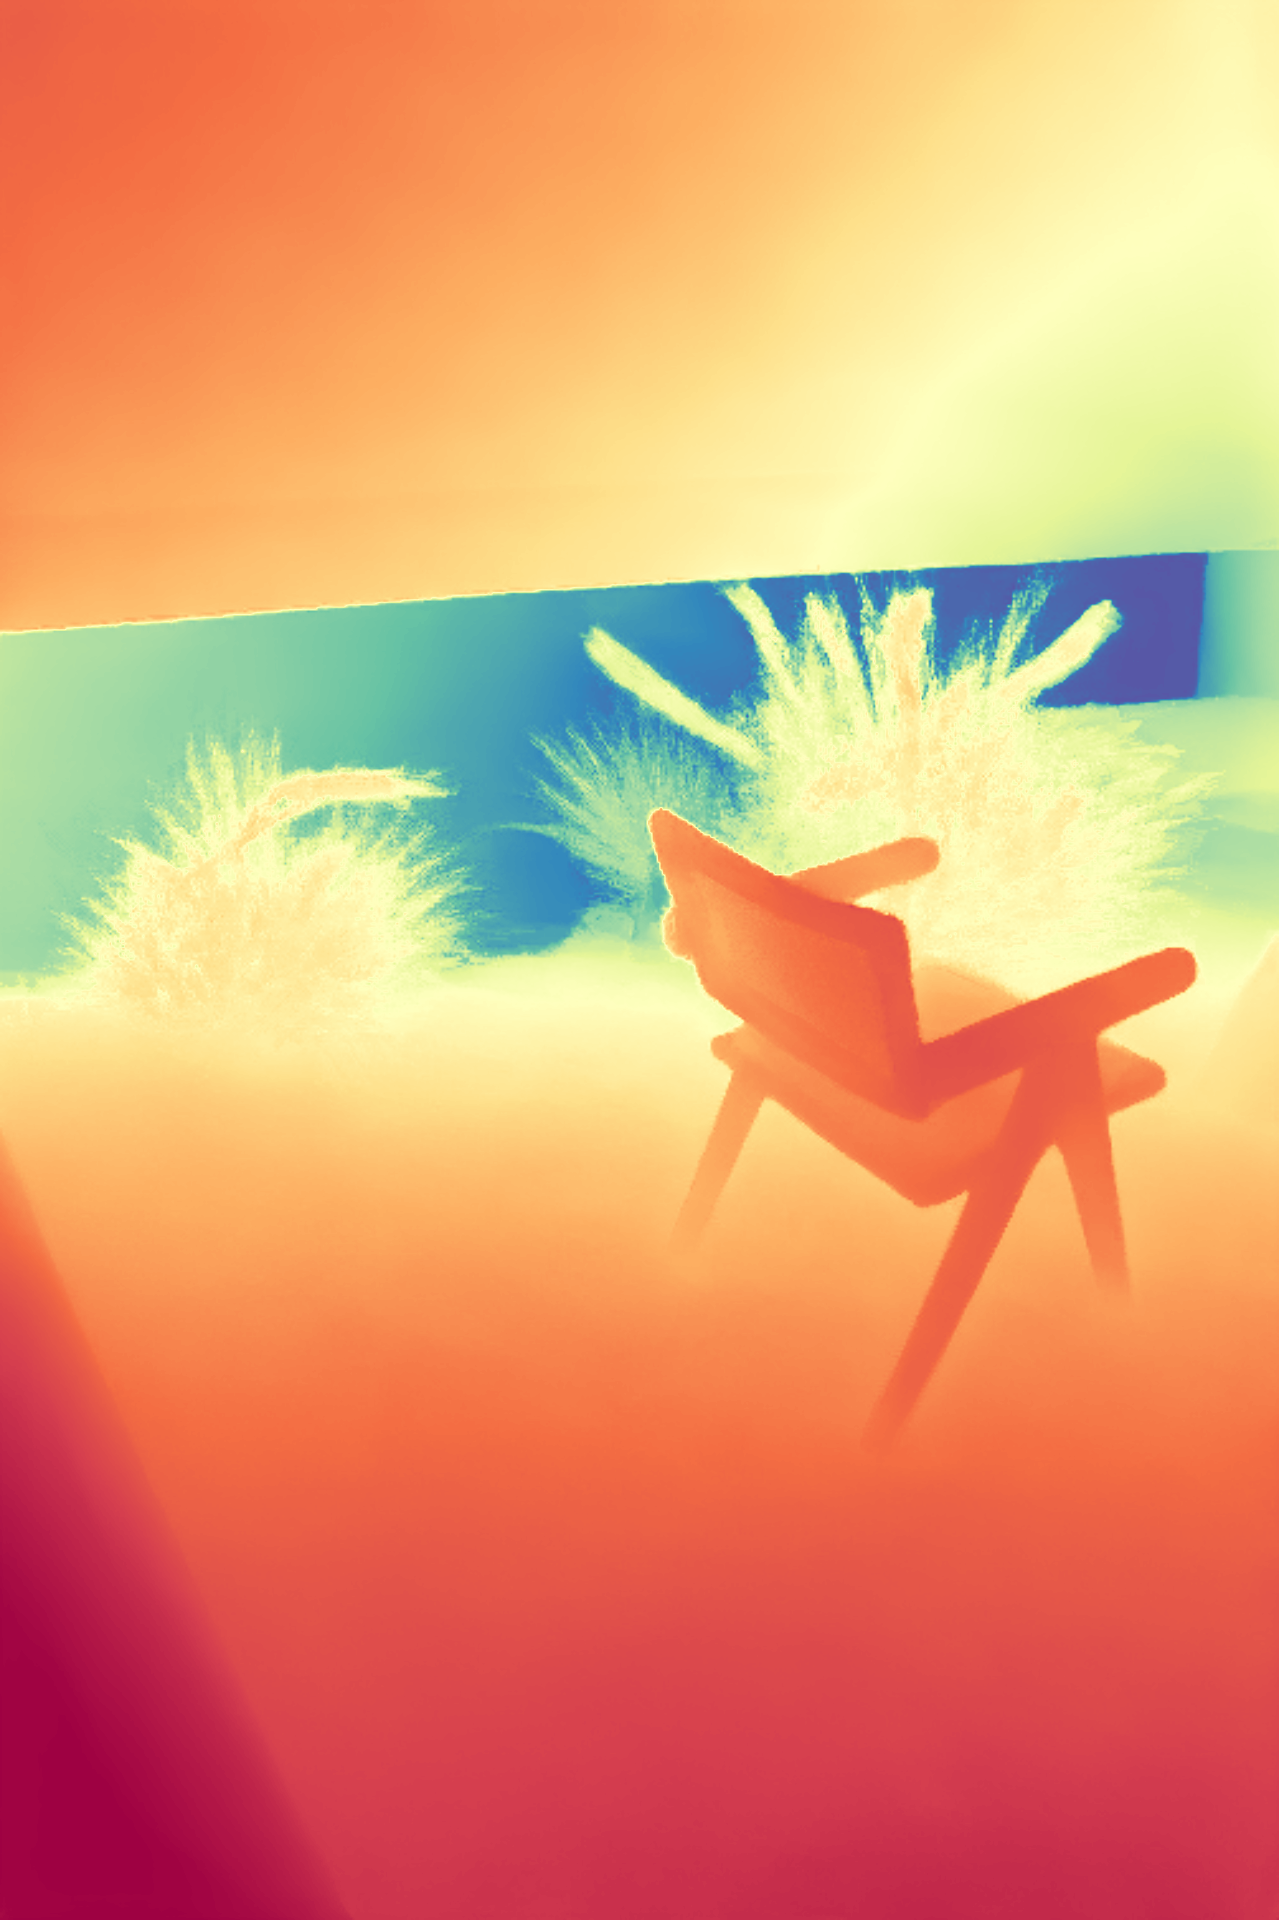
\includegraphics[width=0.2\textwidth]{images/trained/inside-02_pred_colored.png} &
    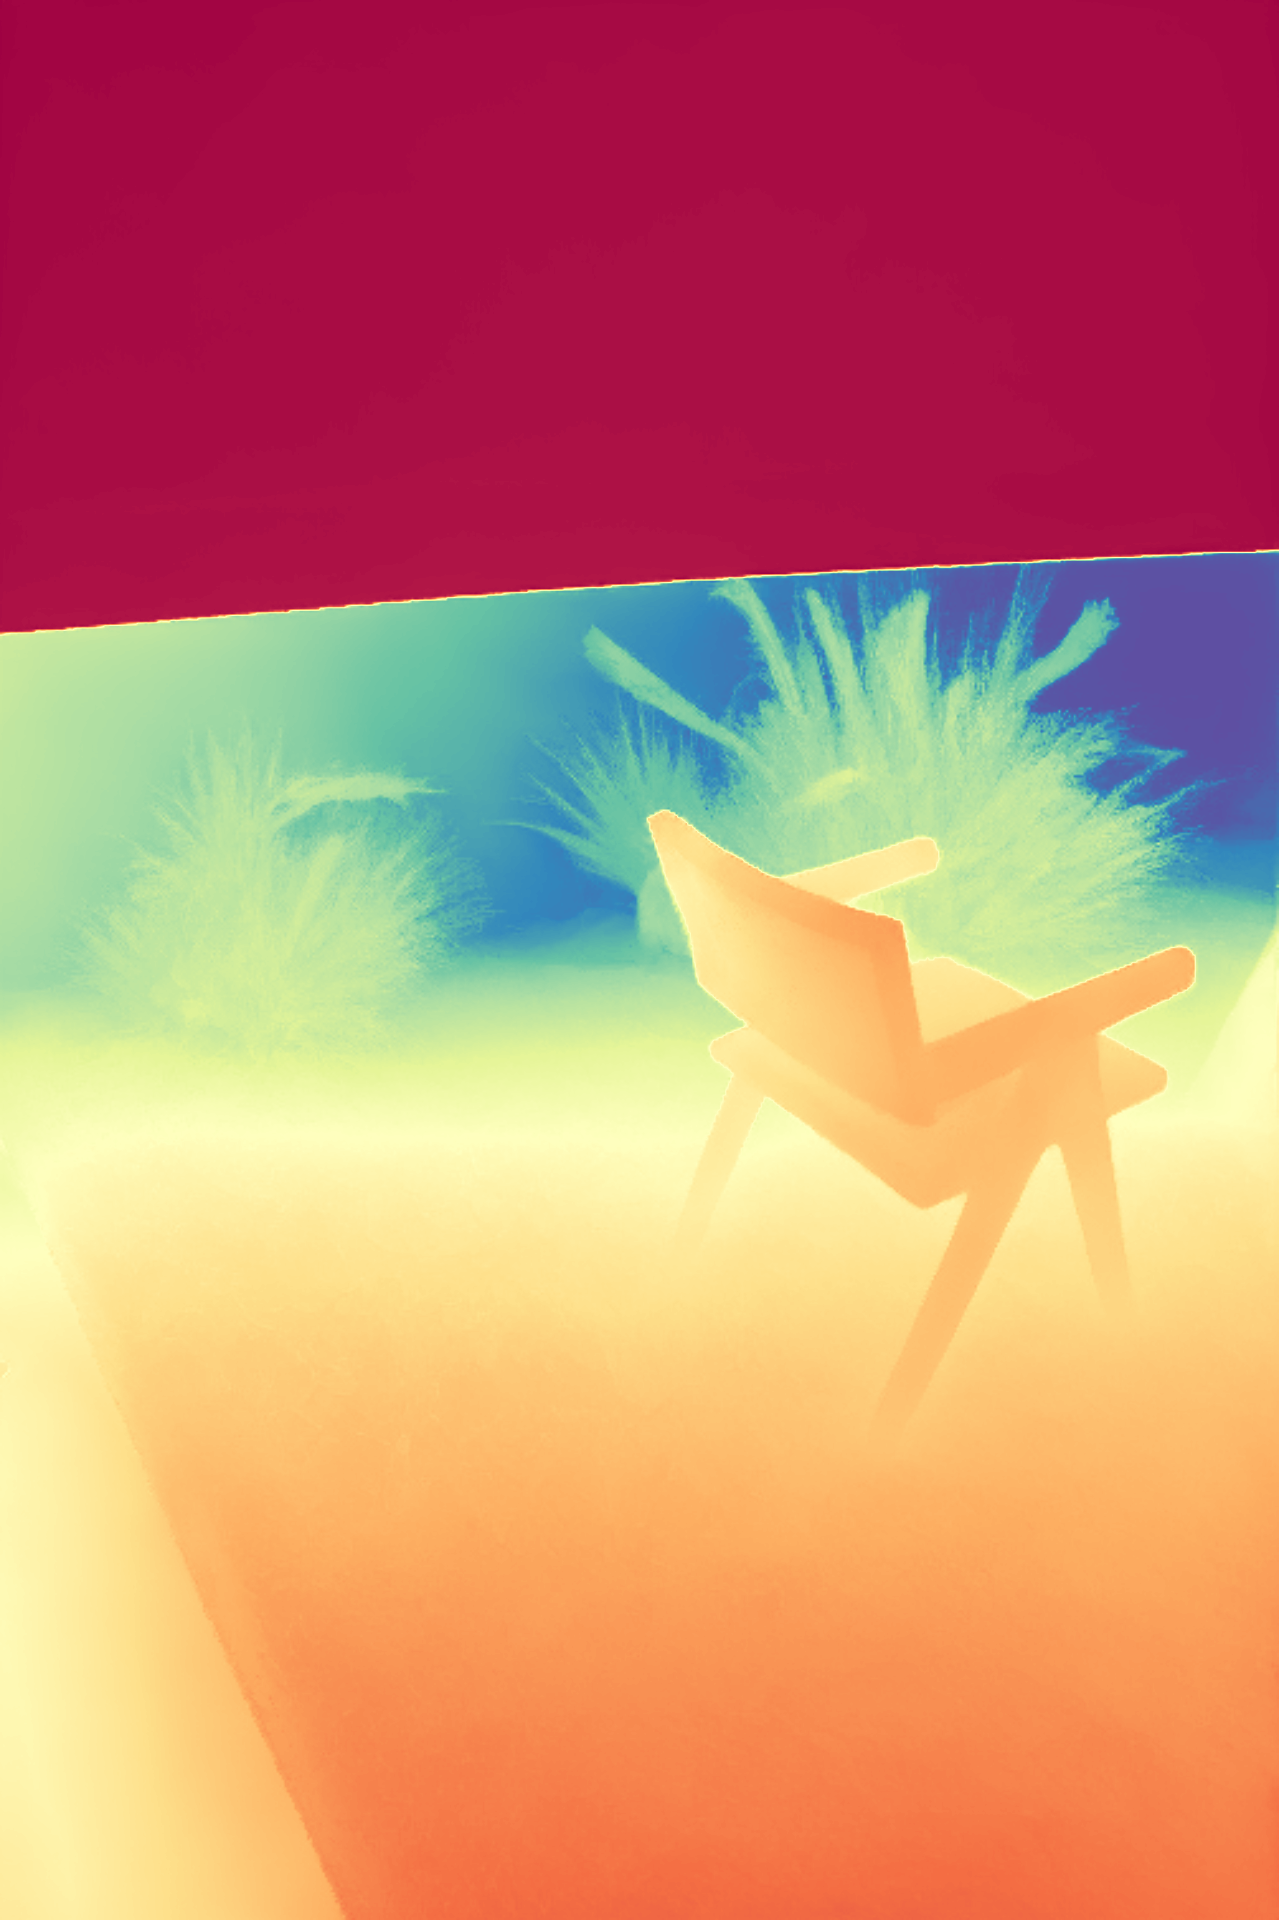
\includegraphics[width=0.2\textwidth]{images/pretrained/inside-02_pred_colored.png} &
    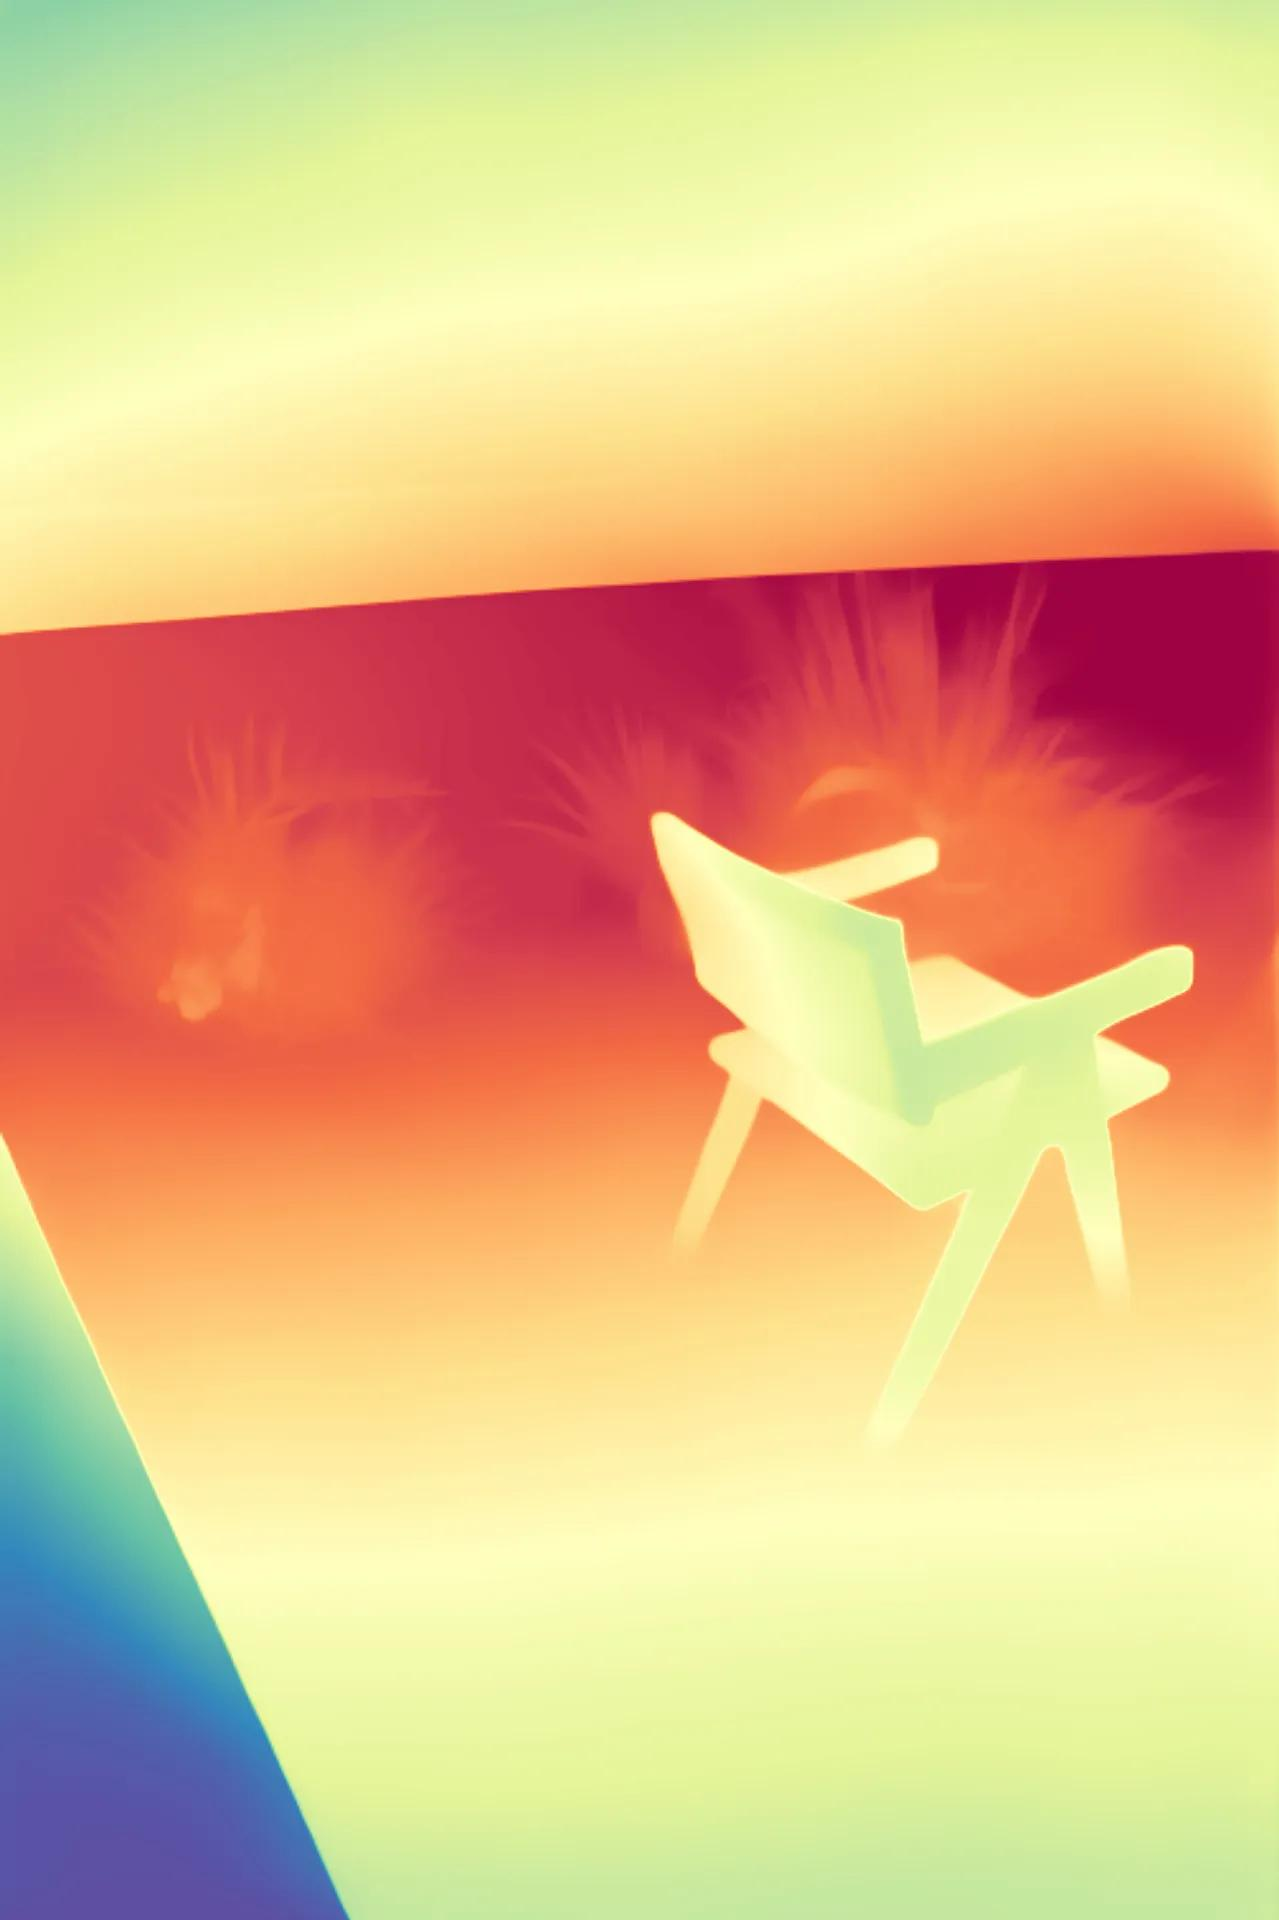
\includegraphics[width=0.2\textwidth]{images/depthmaster/inside-02_pred_colored.jpg} \\

    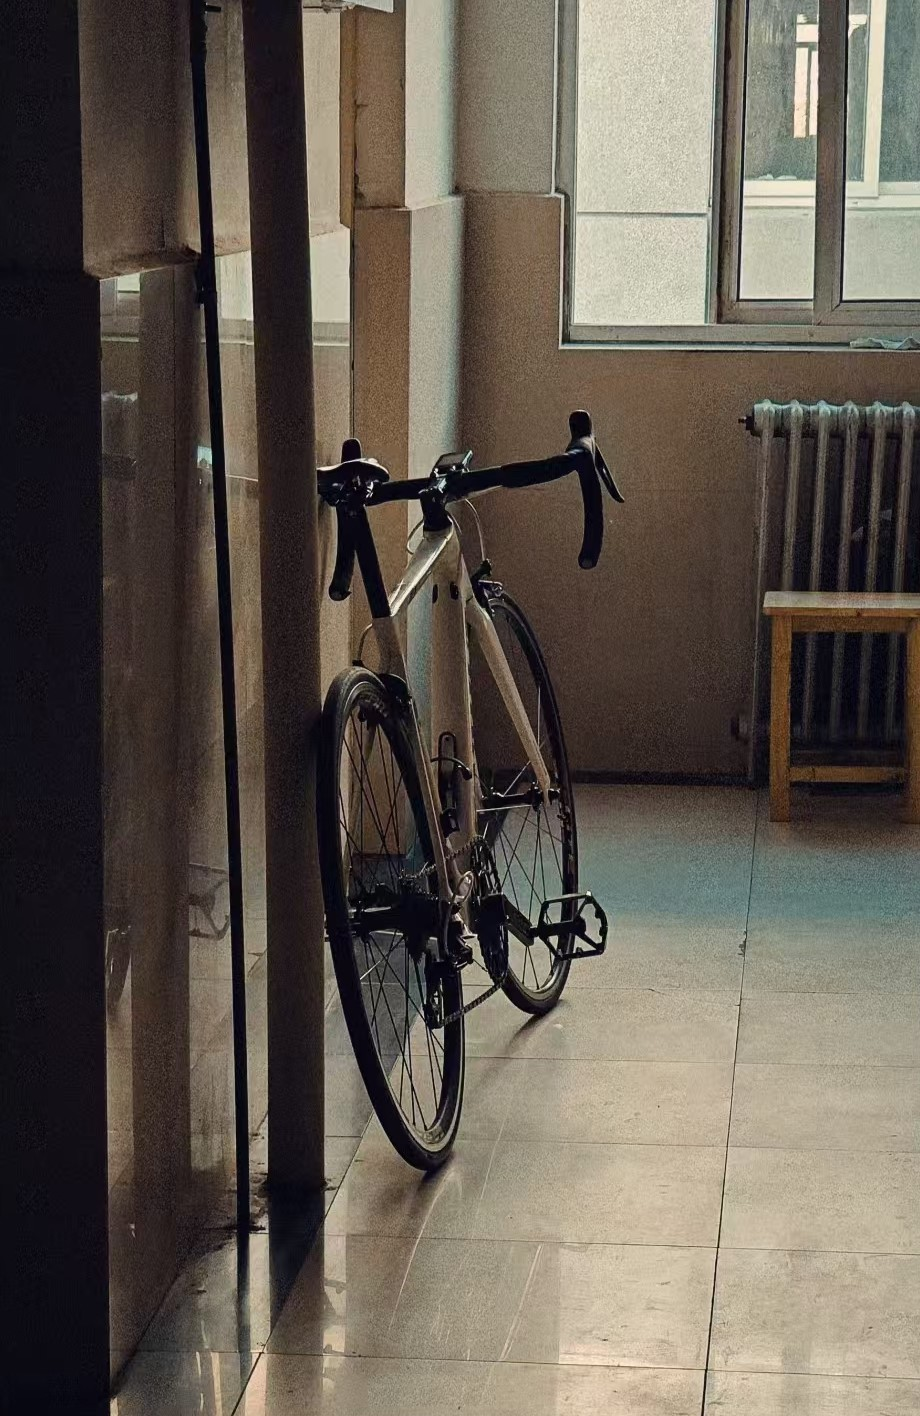
\includegraphics[width=0.2\textwidth]{images/test-image/inside-03.jpg} &
    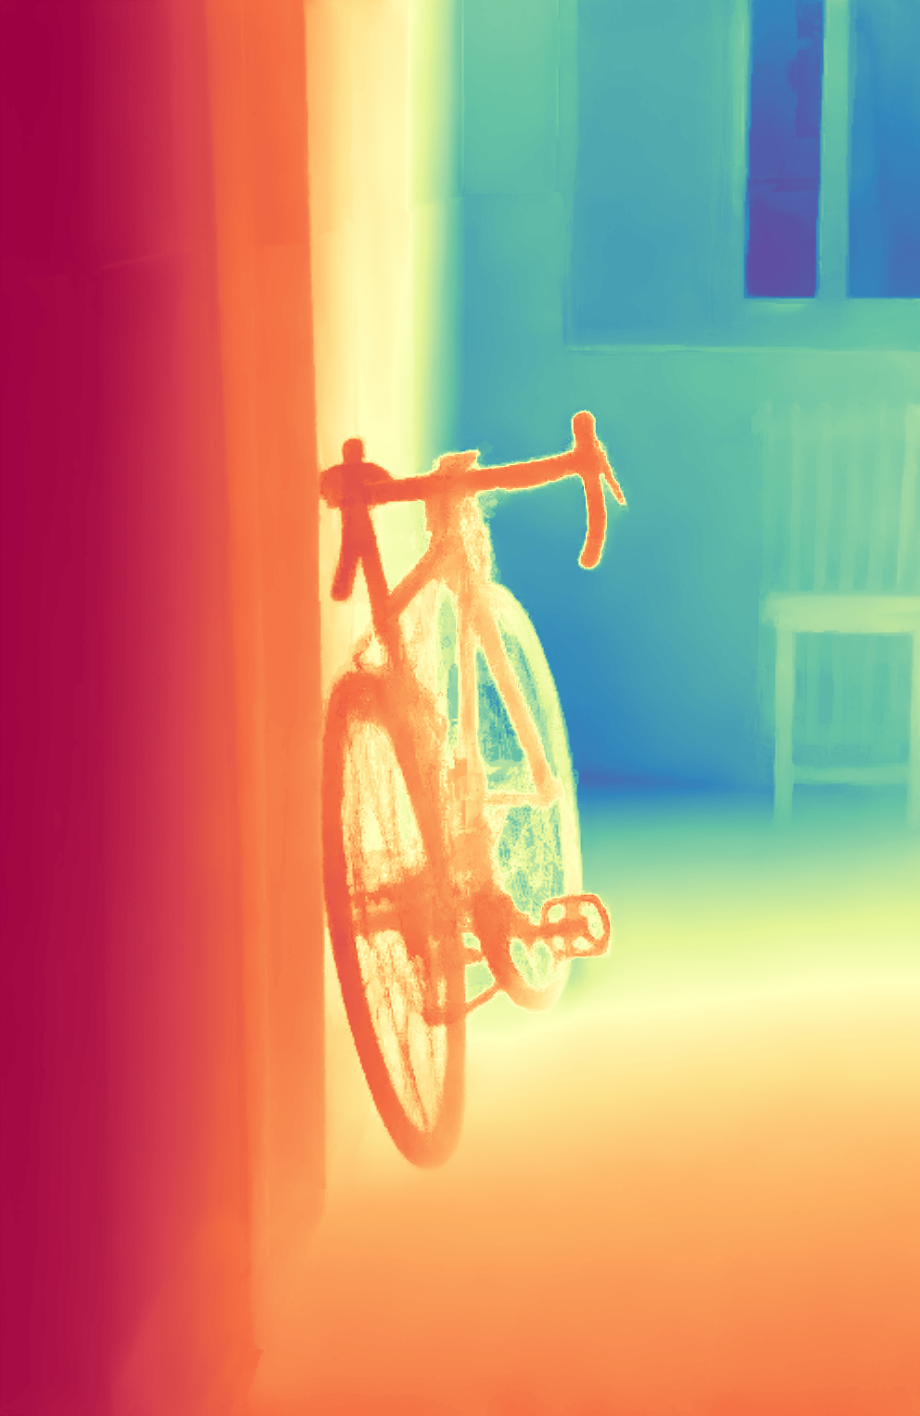
\includegraphics[width=0.2\textwidth]{images/trained/inside-03_pred_colored.png} &
    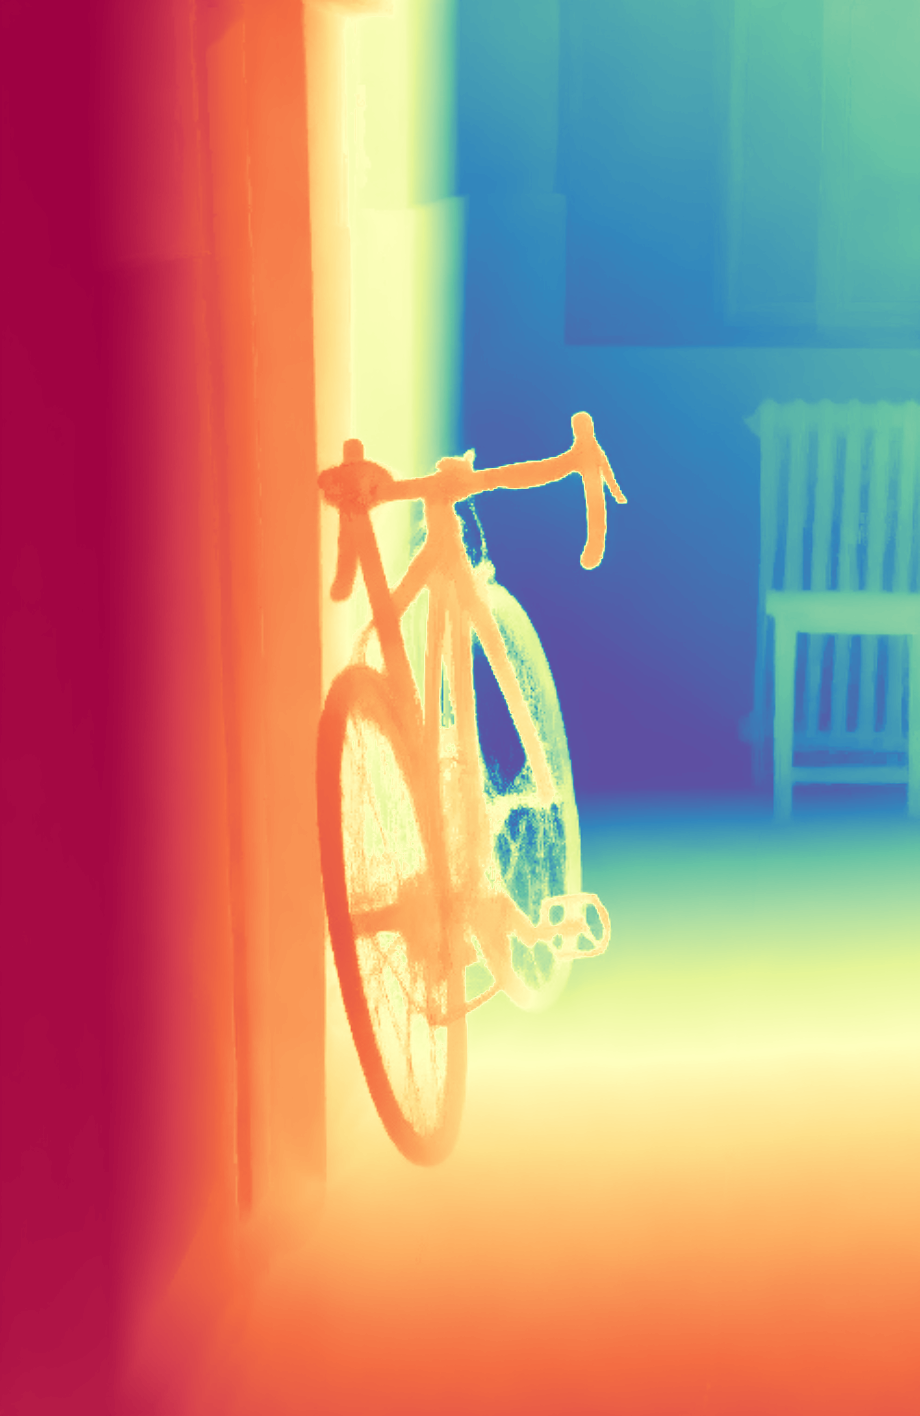
\includegraphics[width=0.2\textwidth]{images/pretrained/inside-03_pred_colored.png} &
    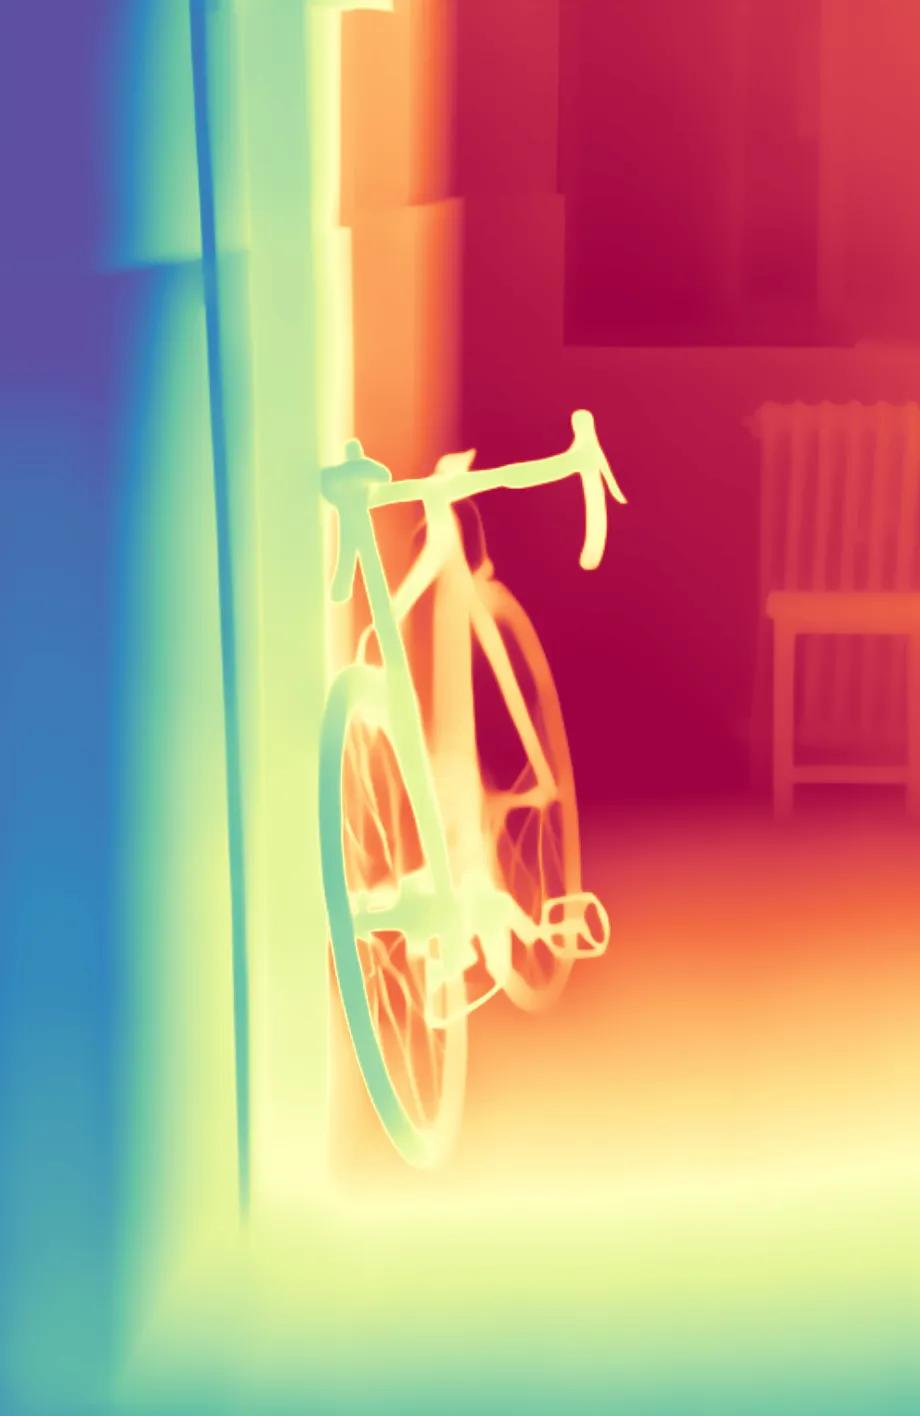
\includegraphics[width=0.2\textwidth]{images/depthmaster/inside-03_pred_colored.jpg} \\

    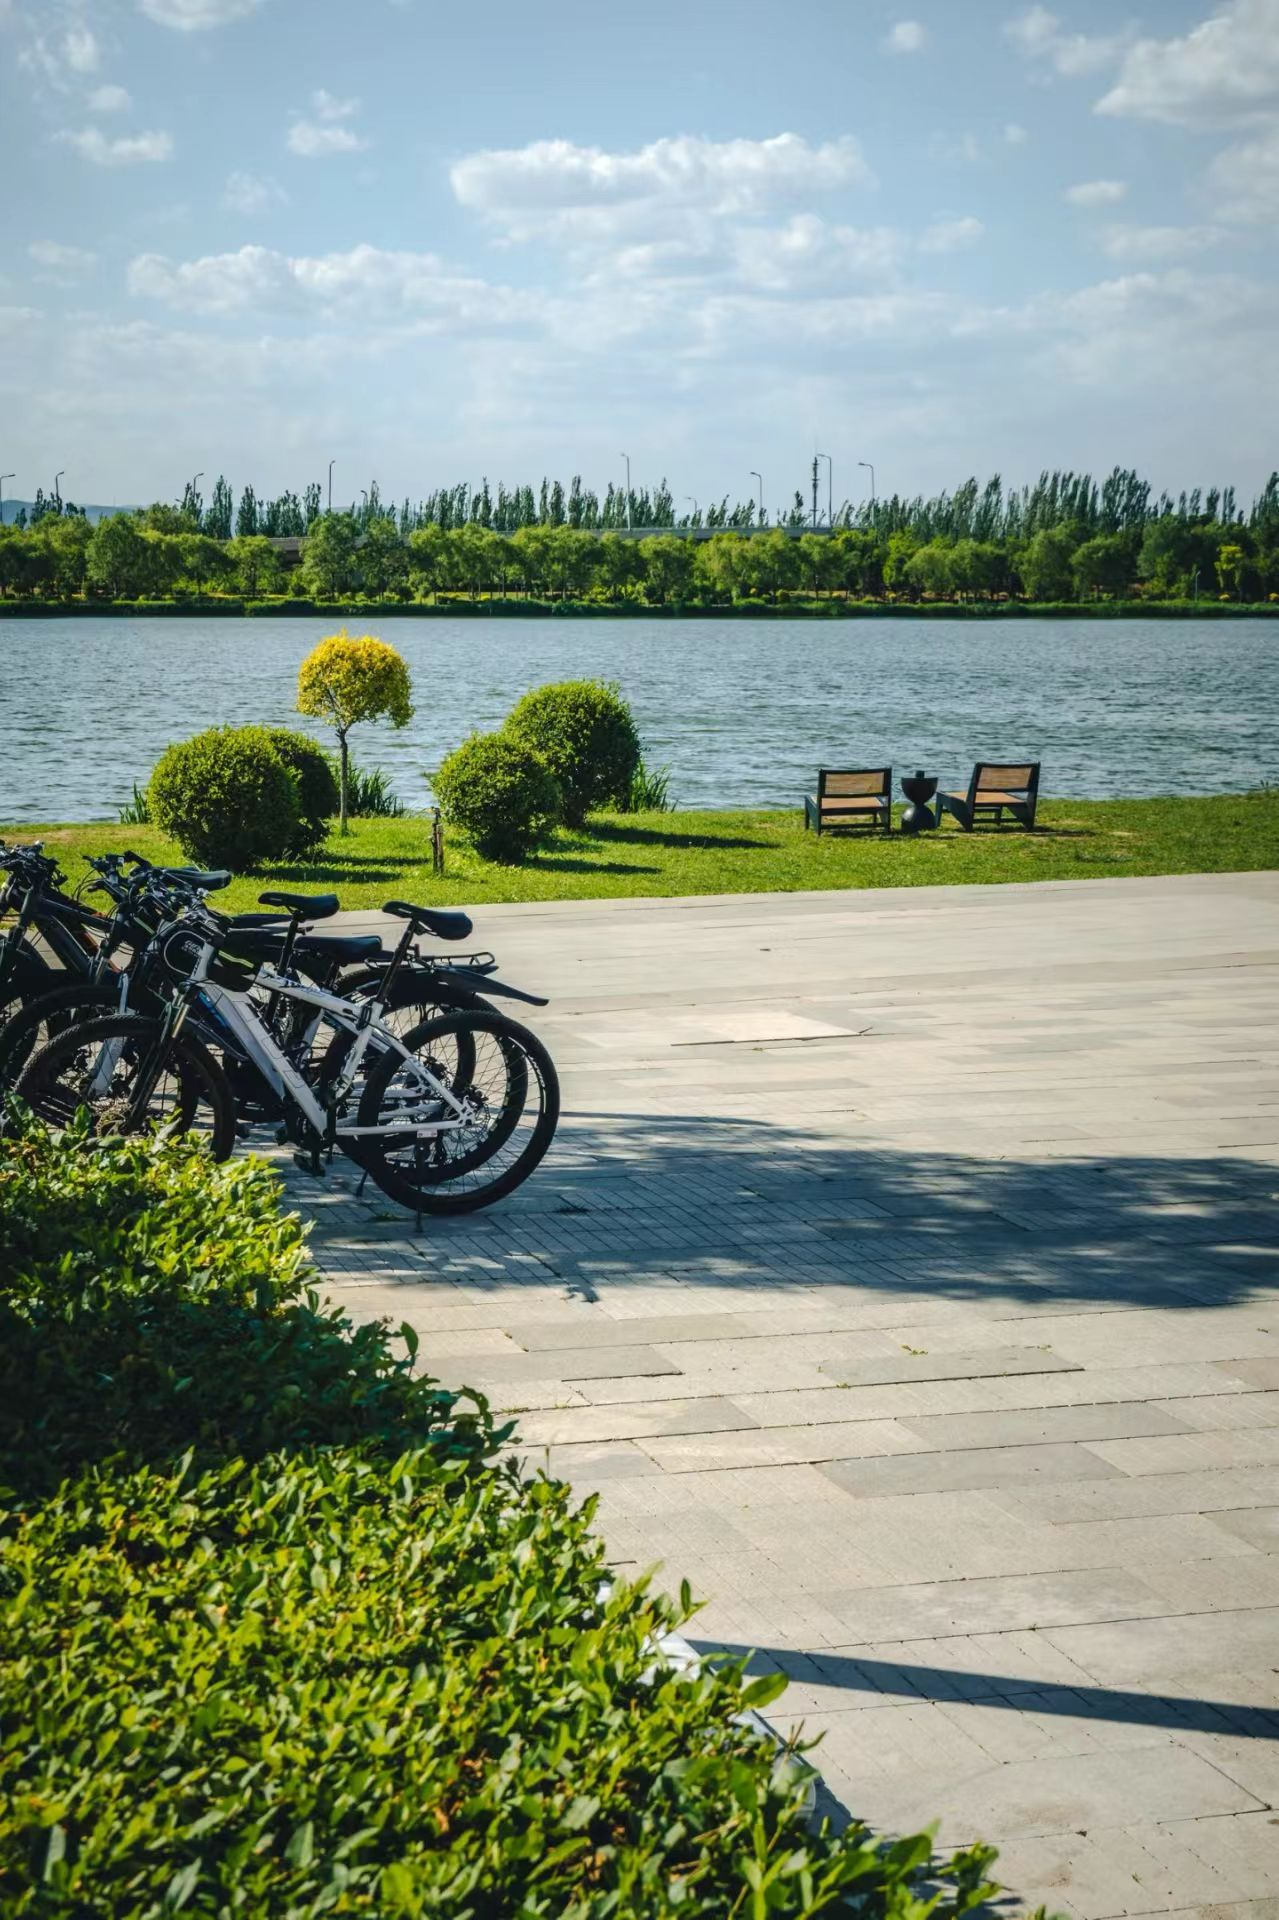
\includegraphics[width=0.2\textwidth]{images/test-image/outside-01.jpg} &
    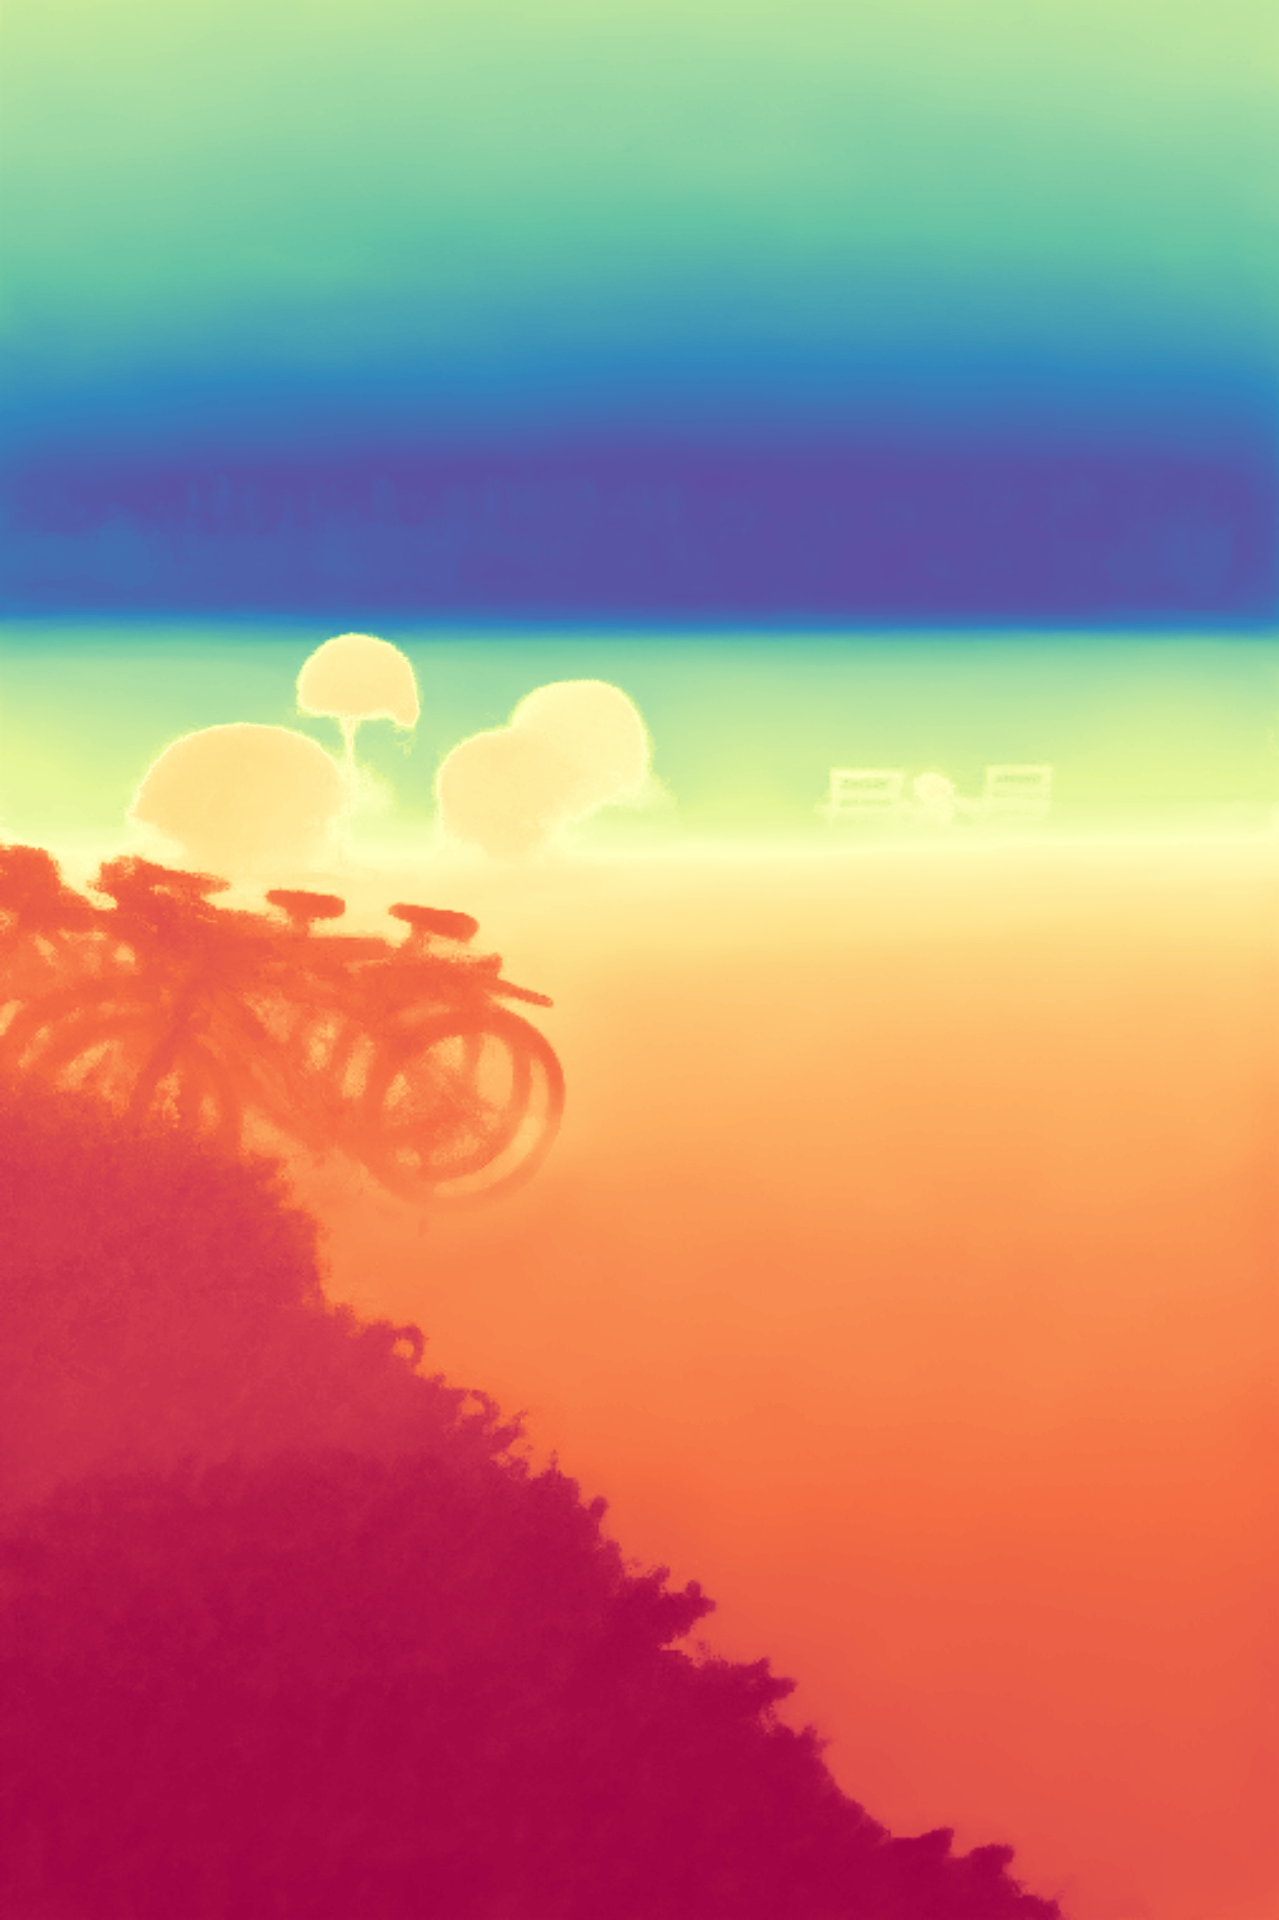
\includegraphics[width=0.2\textwidth]{images/trained/outside-01_pred_colored.png} &
    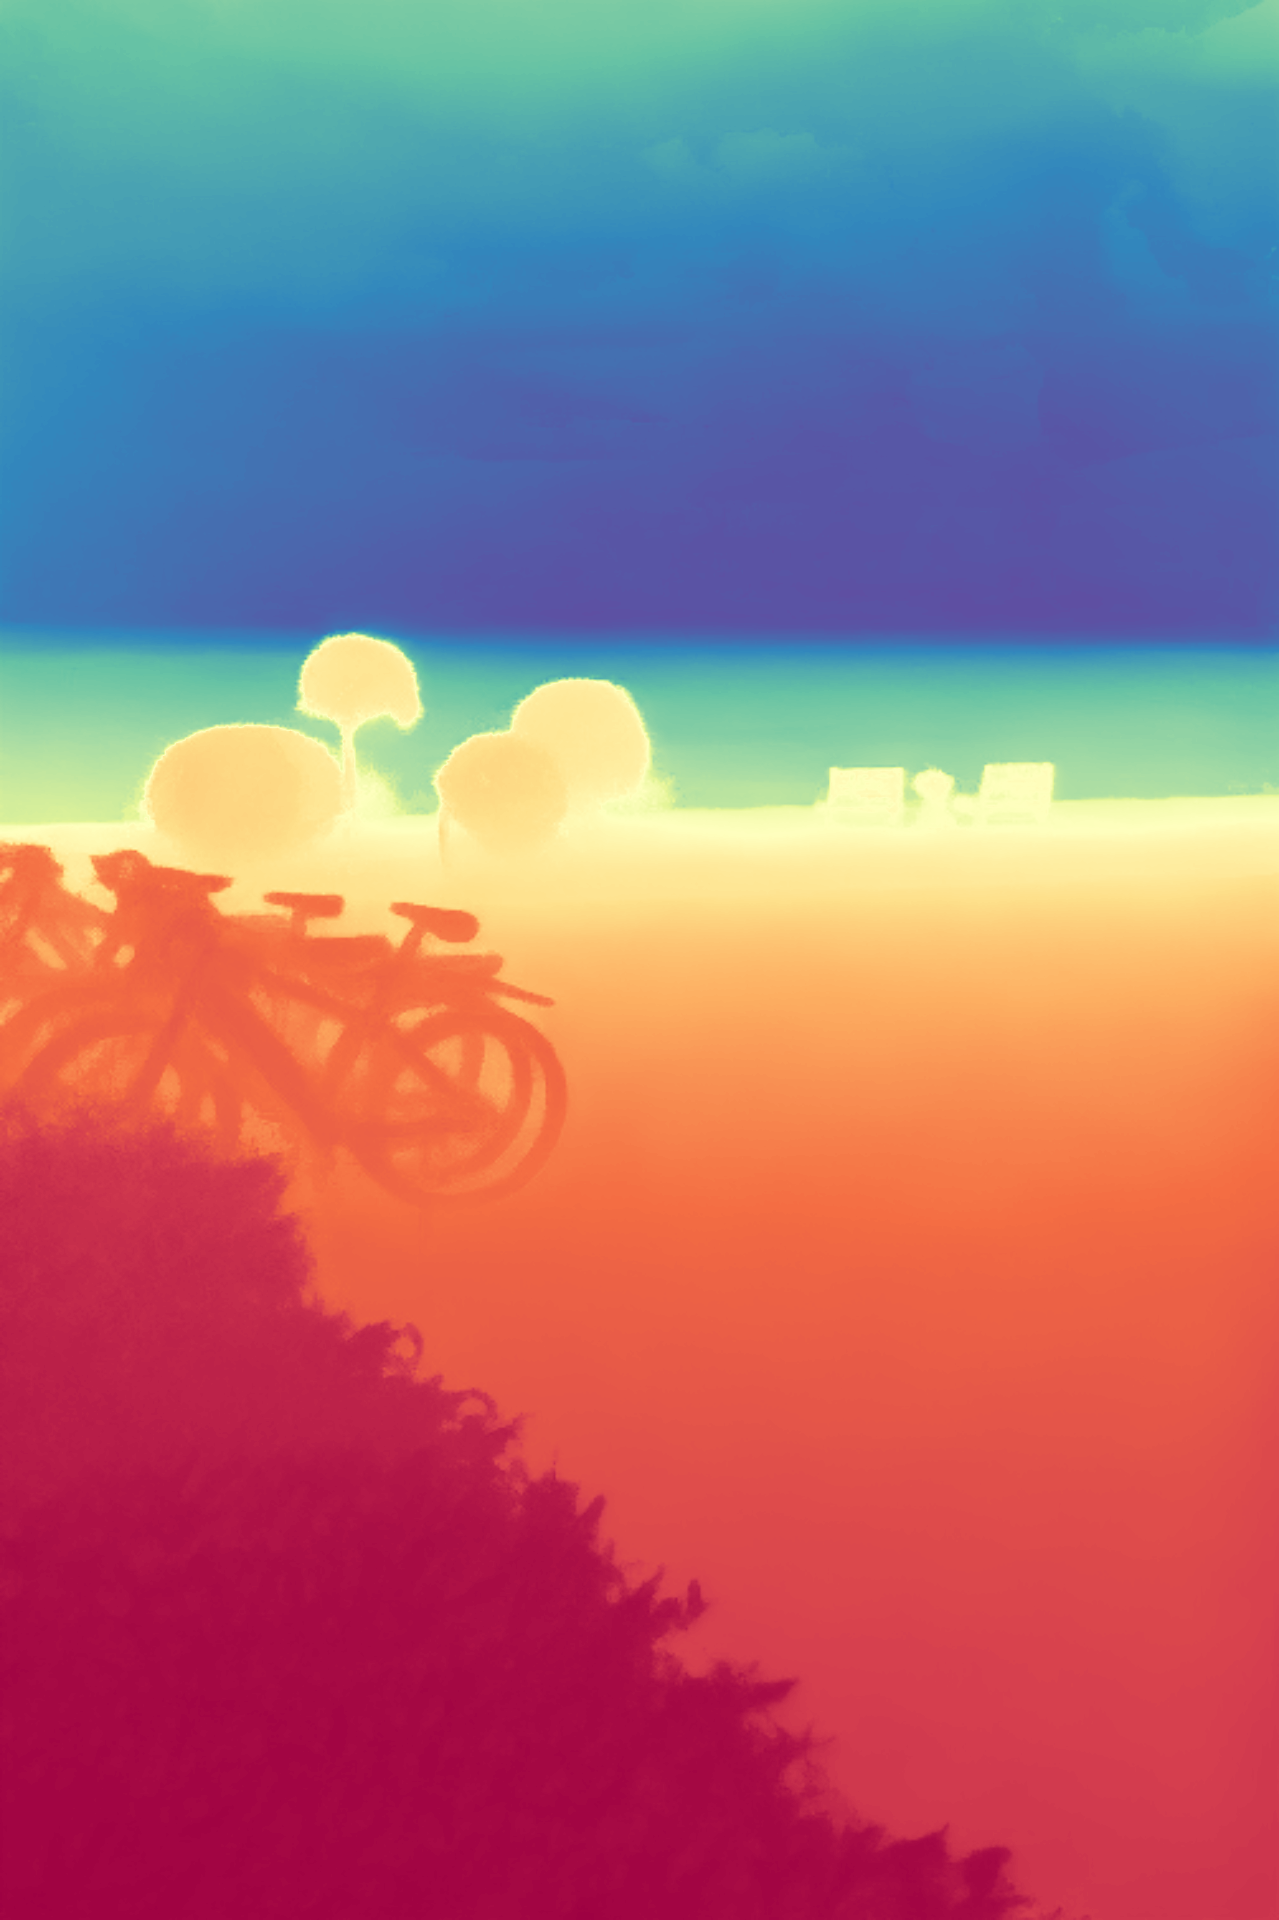
\includegraphics[width=0.2\textwidth]{images/pretrained/outside-01_pred_colored.png} &
    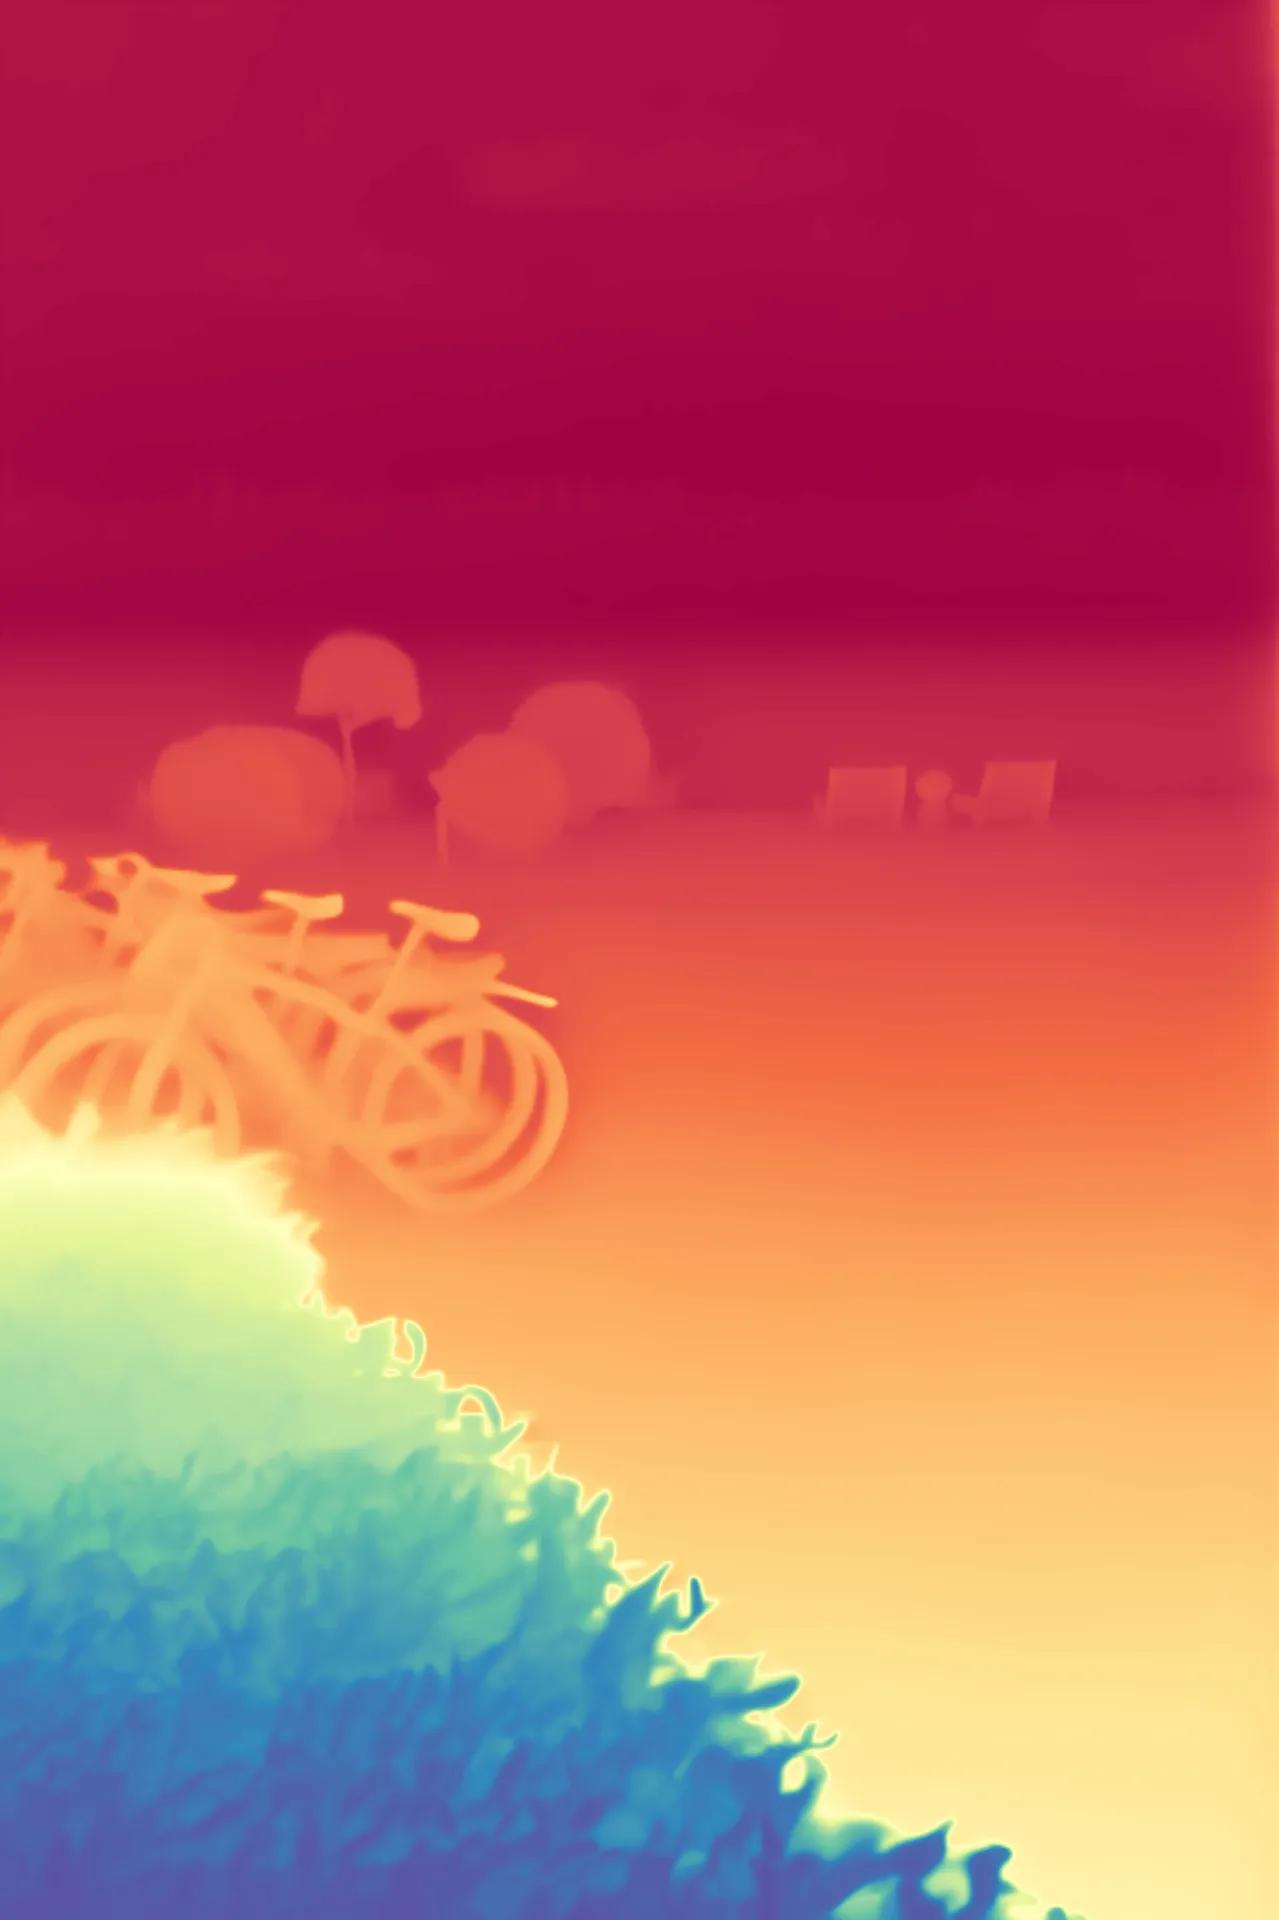
\includegraphics[width=0.2\textwidth]{images/depthmaster/outside-01_pred_colored.jpg} \\

    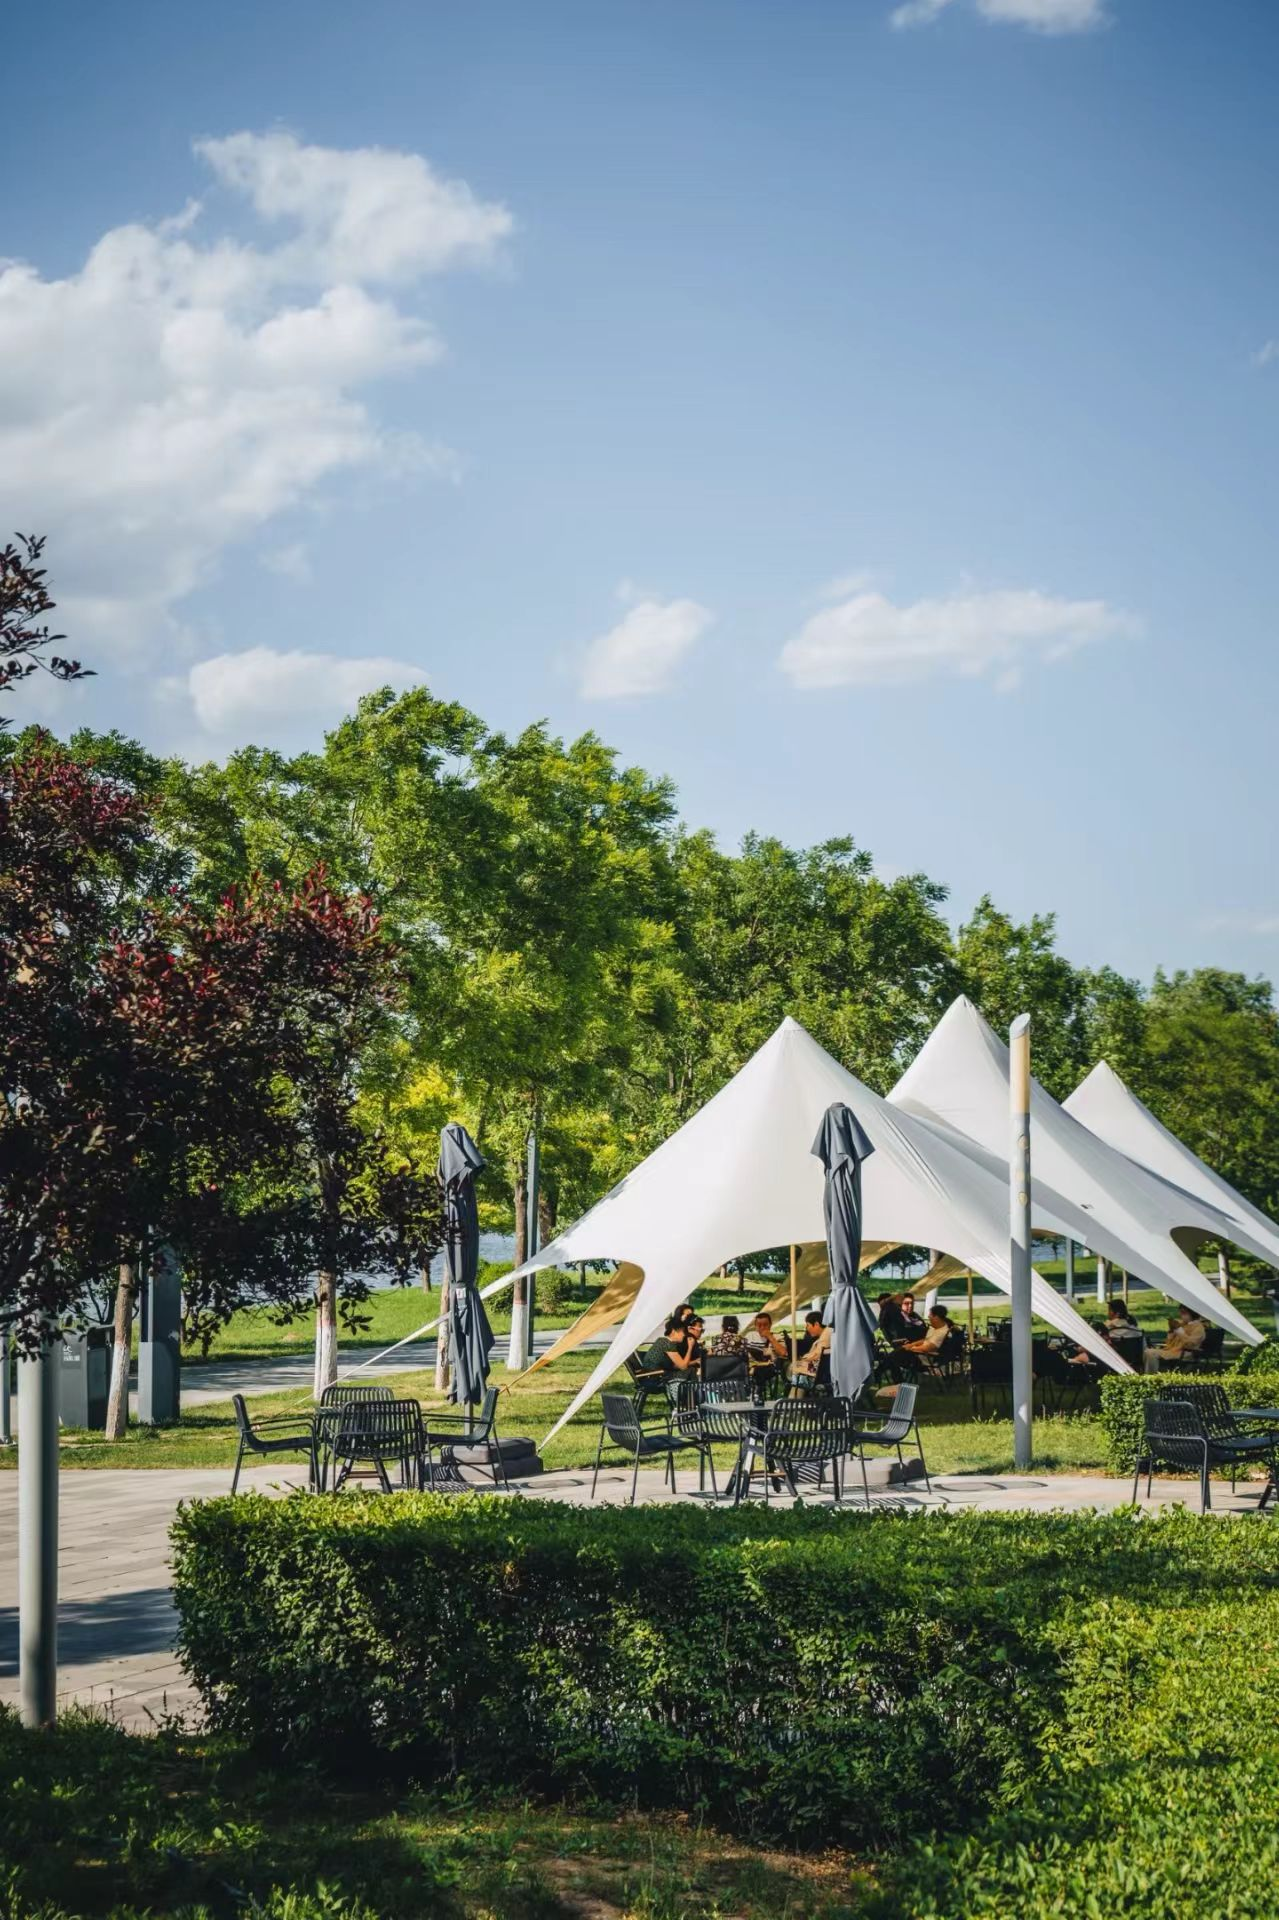
\includegraphics[width=0.2\textwidth]{images/test-image/outside-02.jpg} &
    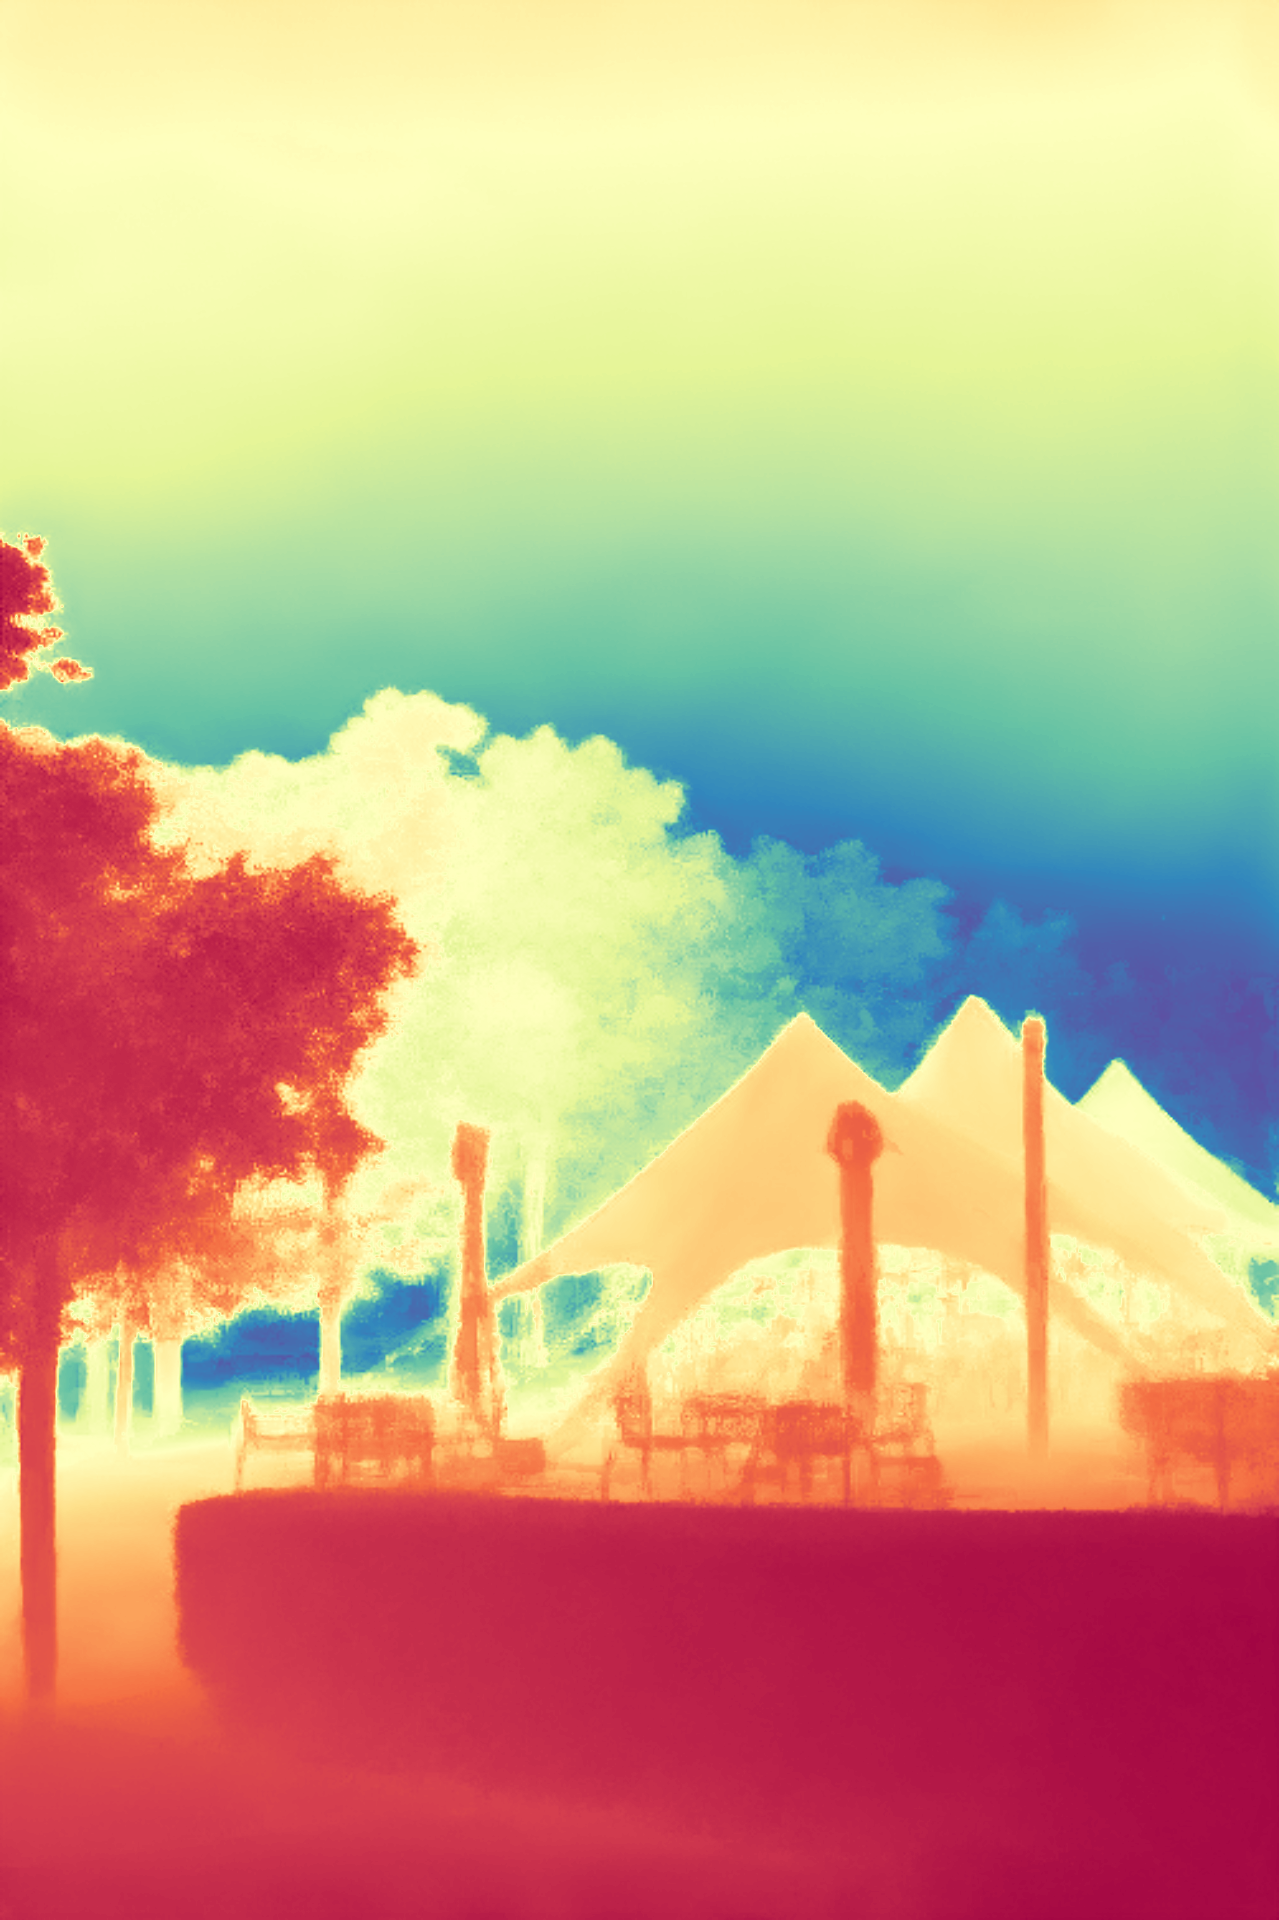
\includegraphics[width=0.2\textwidth]{images/trained/outside-02_pred_colored.png} &
    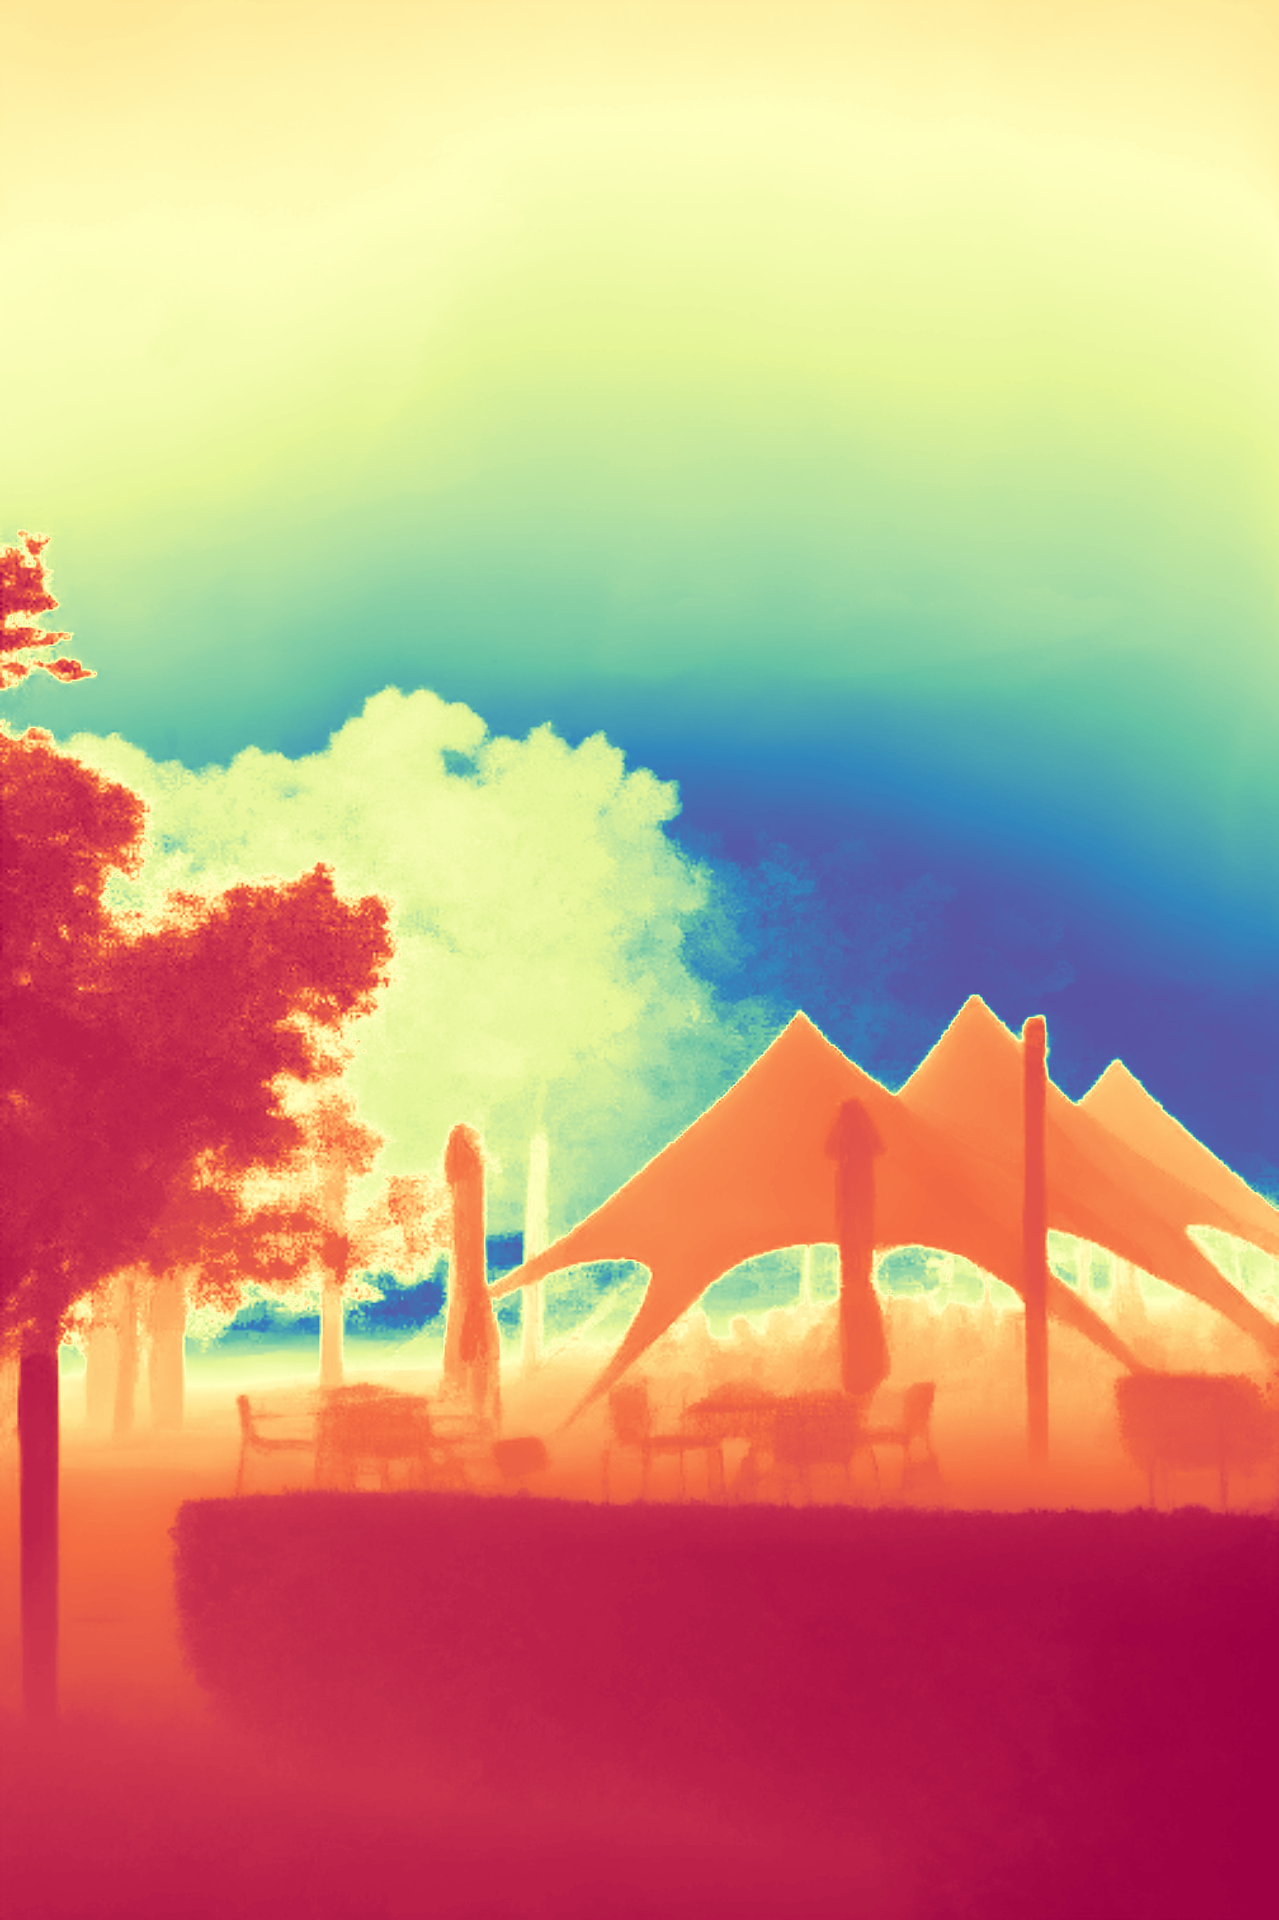
\includegraphics[width=0.2\textwidth]{images/pretrained/outside-02_pred_colored.png} &
    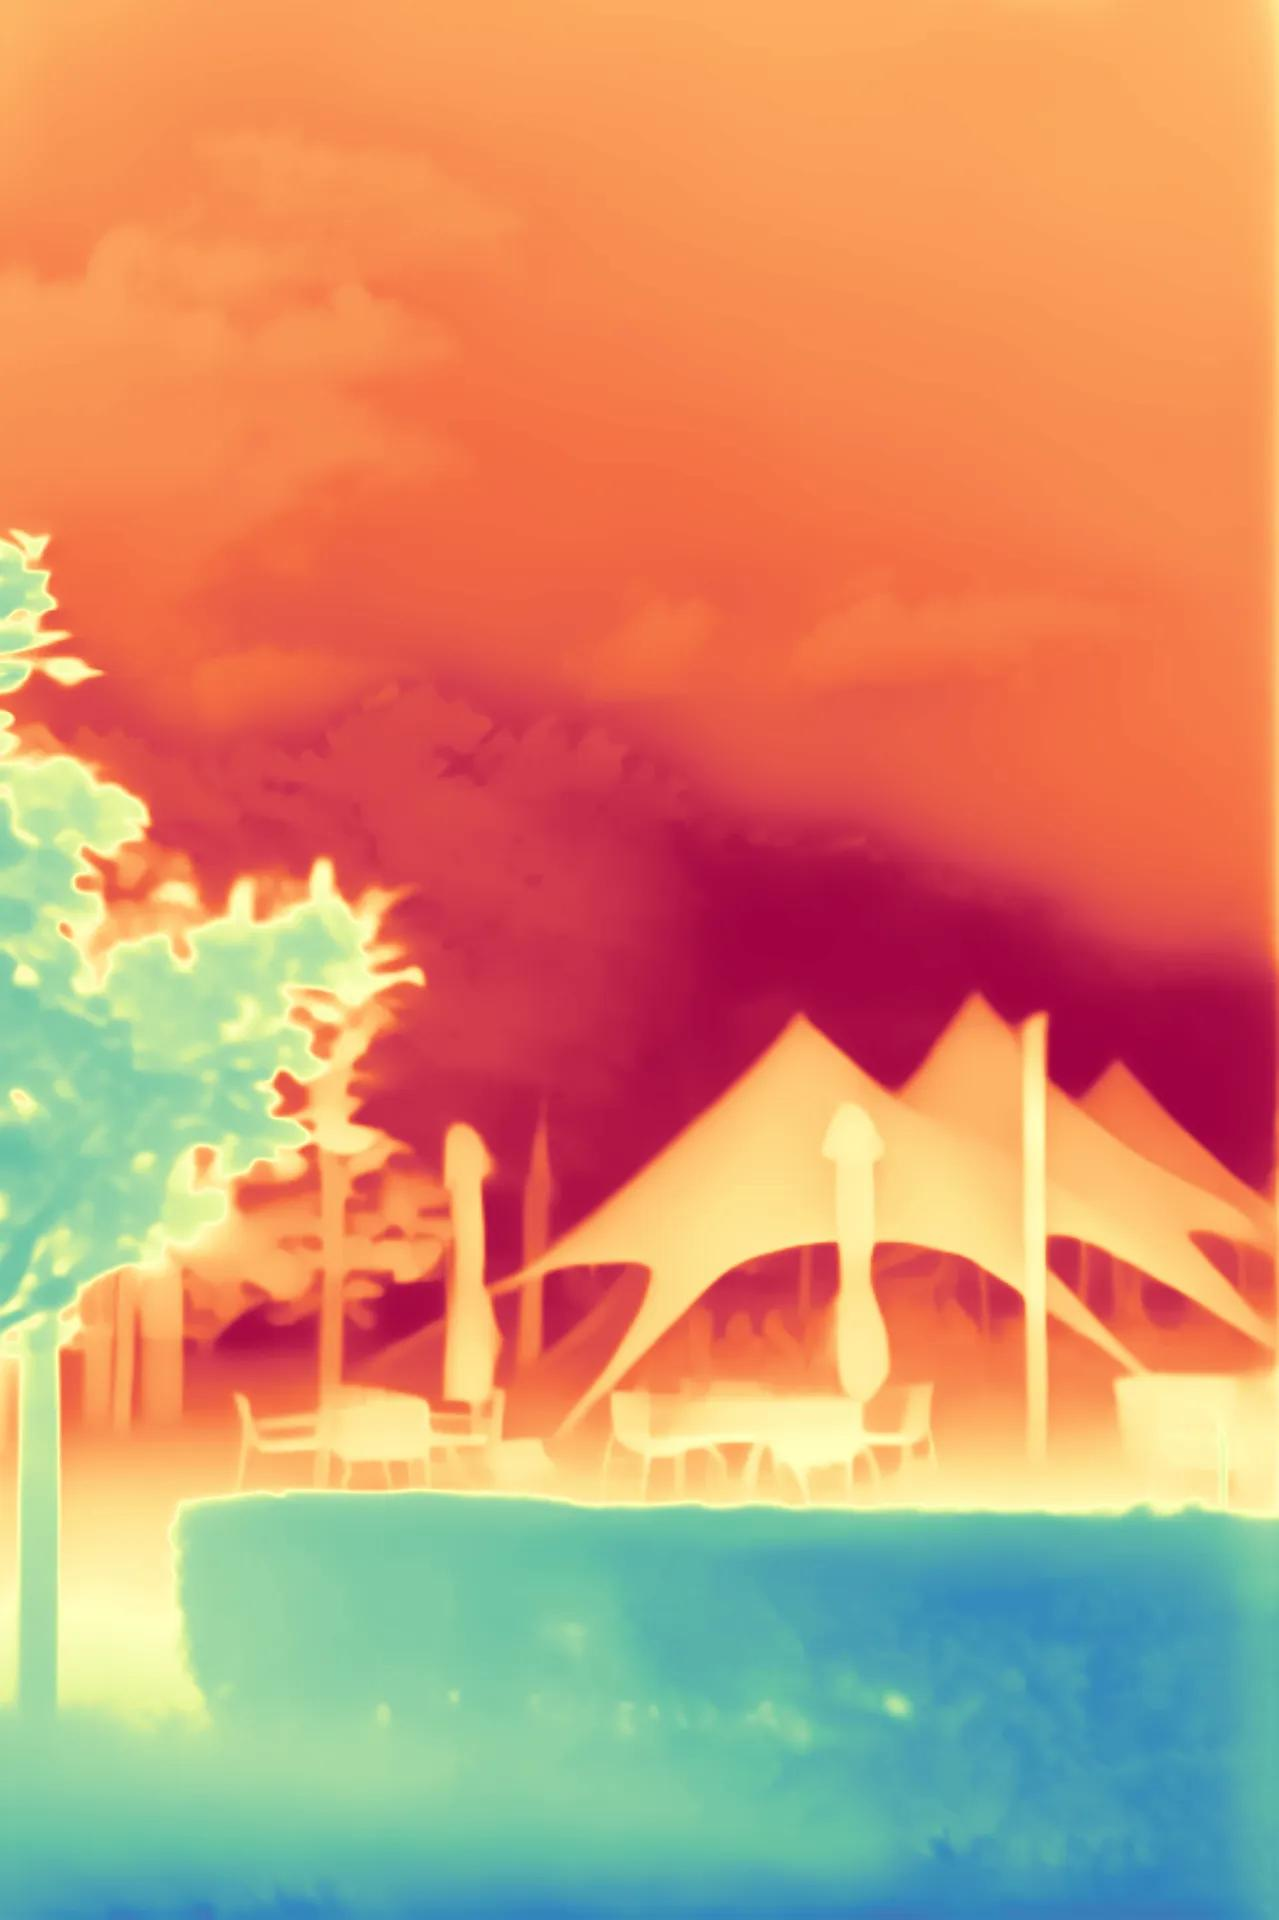
\includegraphics[width=0.2\textwidth]{images/depthmaster/outside-02_pred_colored.jpg} \\
  \end{tabular}
  \caption{原图,自训练模型,\textit{\textbf{Marigold}}与\textit{\textbf{DepthMaster}}的输出结果对比,四张图像均为真实世界的室内、室外图像}
\end{figure}

\newpage

% 第二组图
\begin{figure}[H]
  \centering
  \begin{tabular}{cccc}
    \textbf{Input RGB Image} & \textbf{Trained iter: 3450} & \textbf{Marigold} & \textbf{DepthMaster} \\
    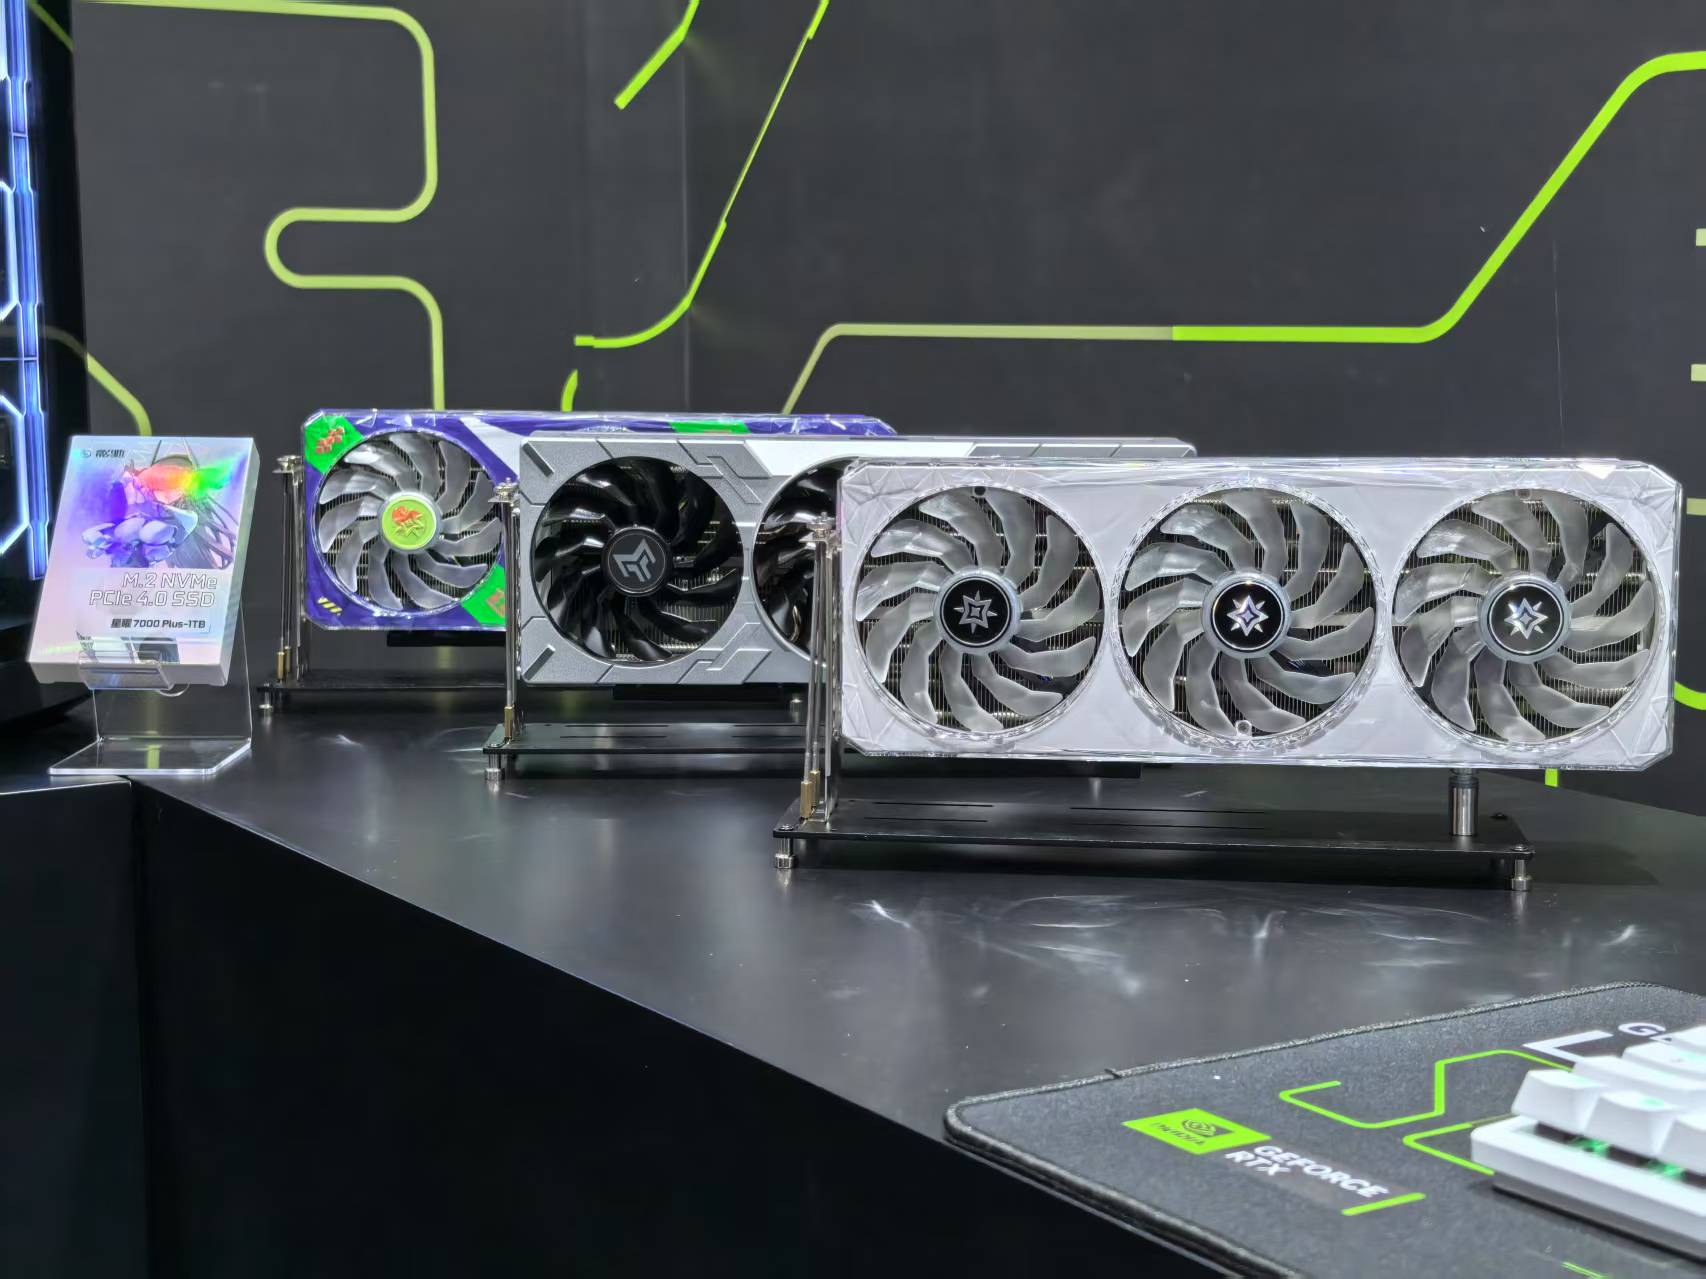
\includegraphics[width=0.22\textwidth]{images/test-image/inside-01.jpg} &
    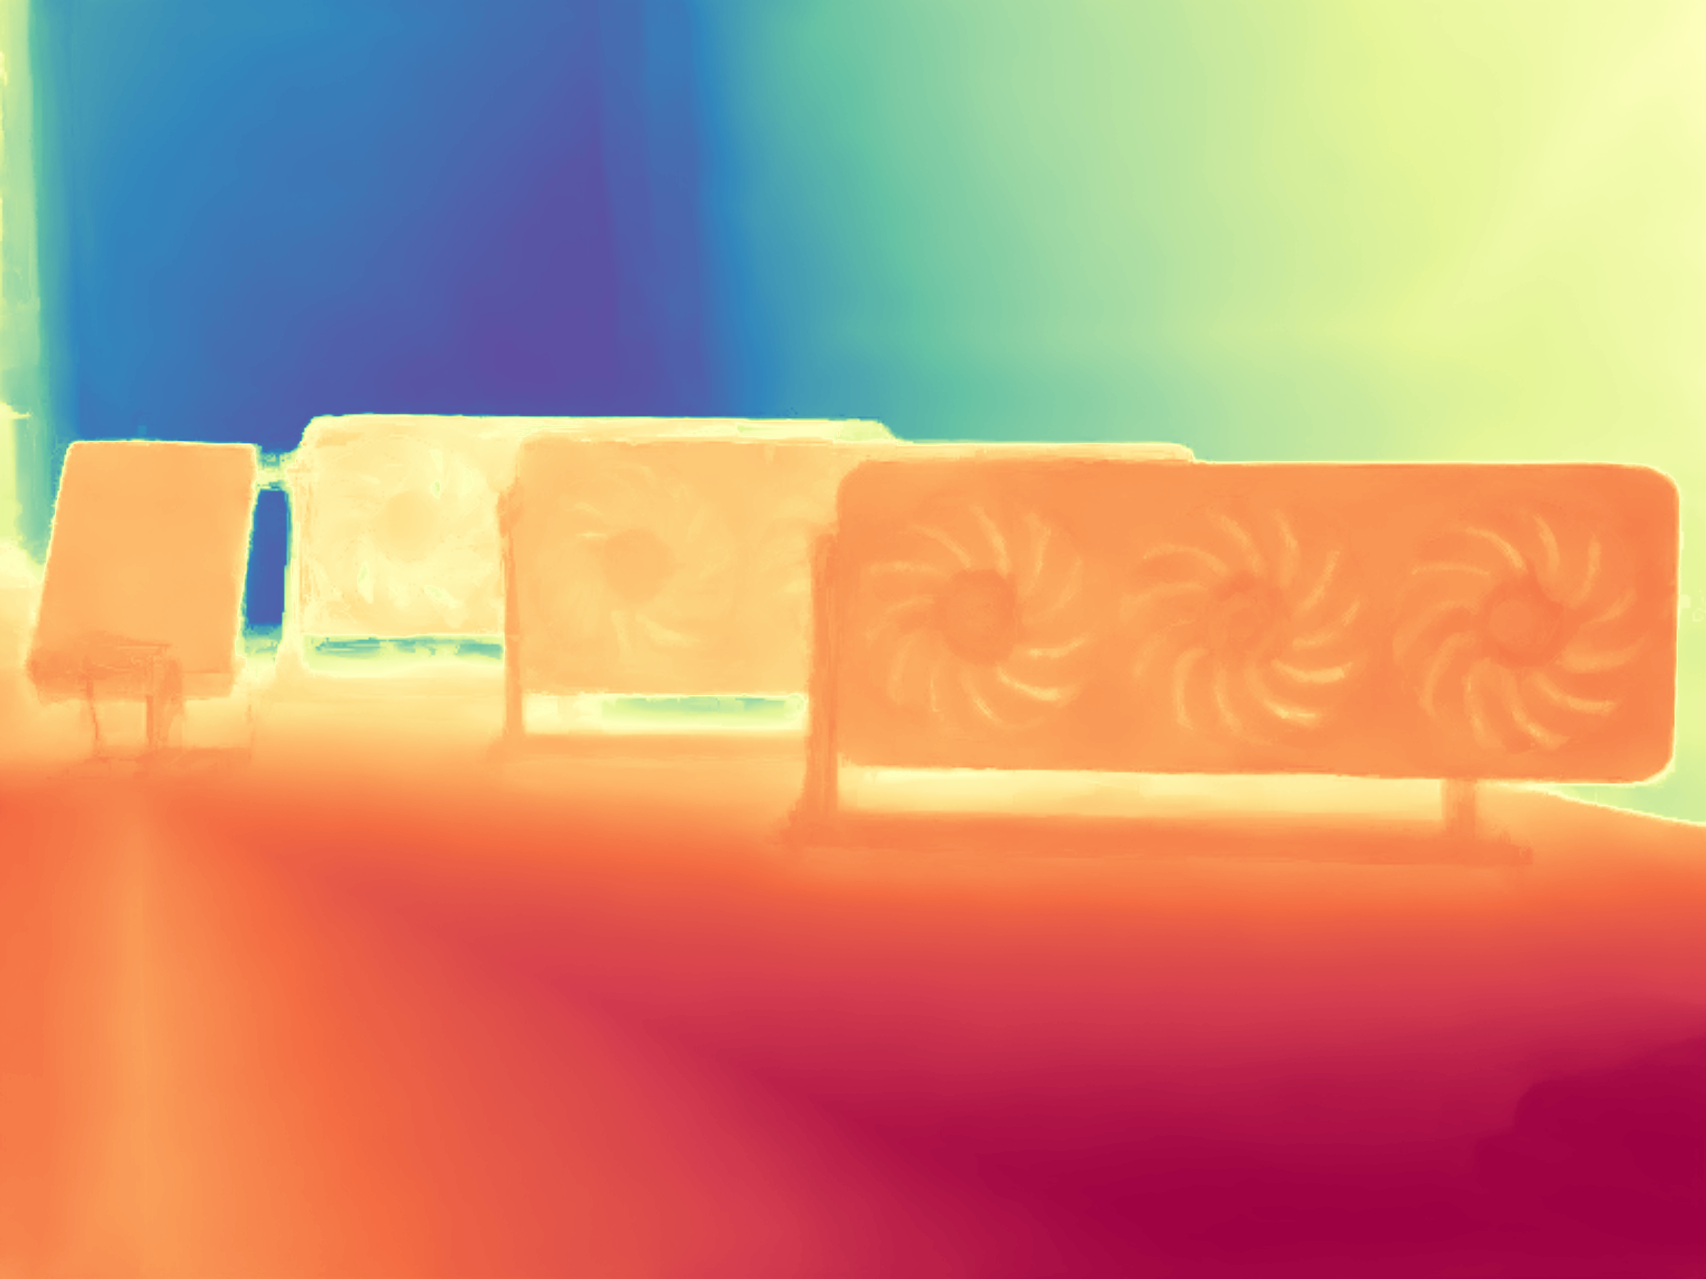
\includegraphics[width=0.22\textwidth]{images/trained/inside-01_pred_colored.png} &
    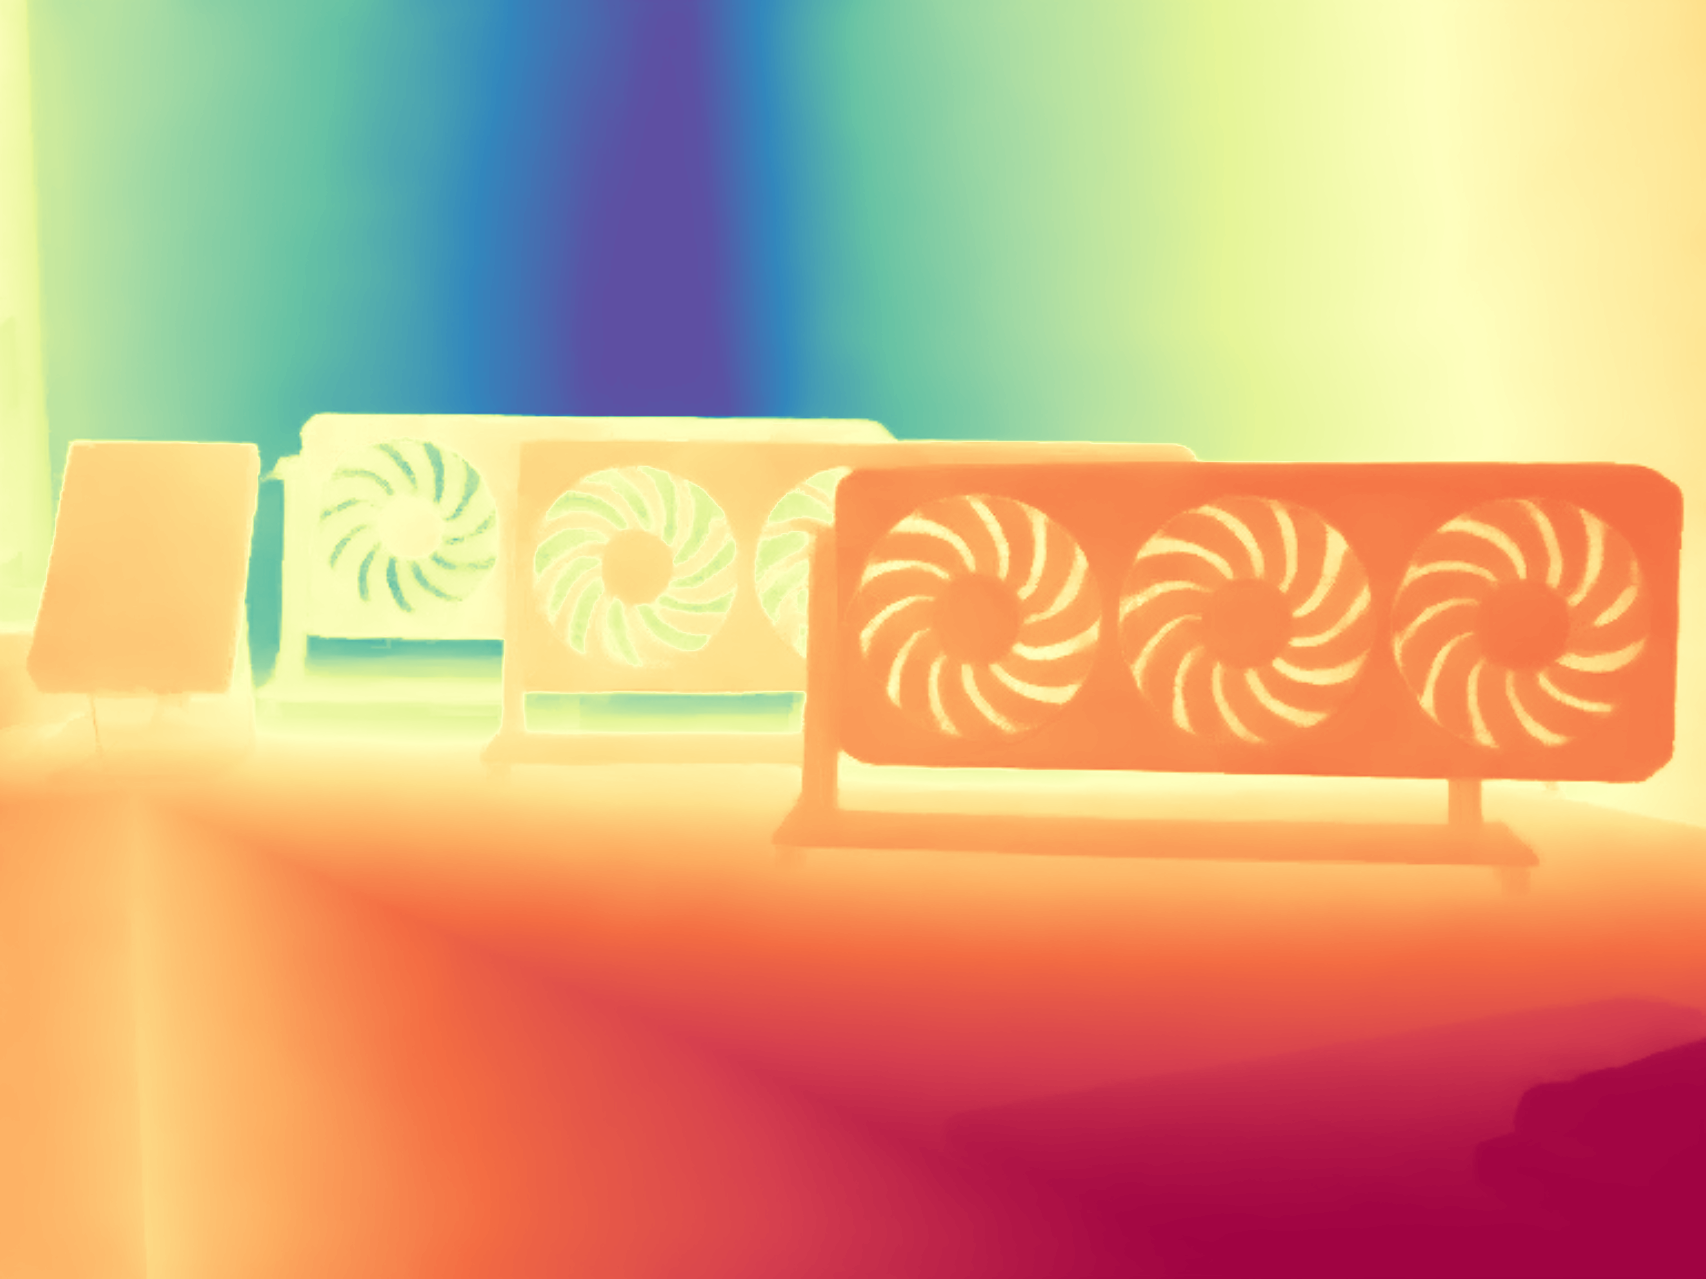
\includegraphics[width=0.22\textwidth]{images/pretrained/inside-01_pred_colored.png} &
    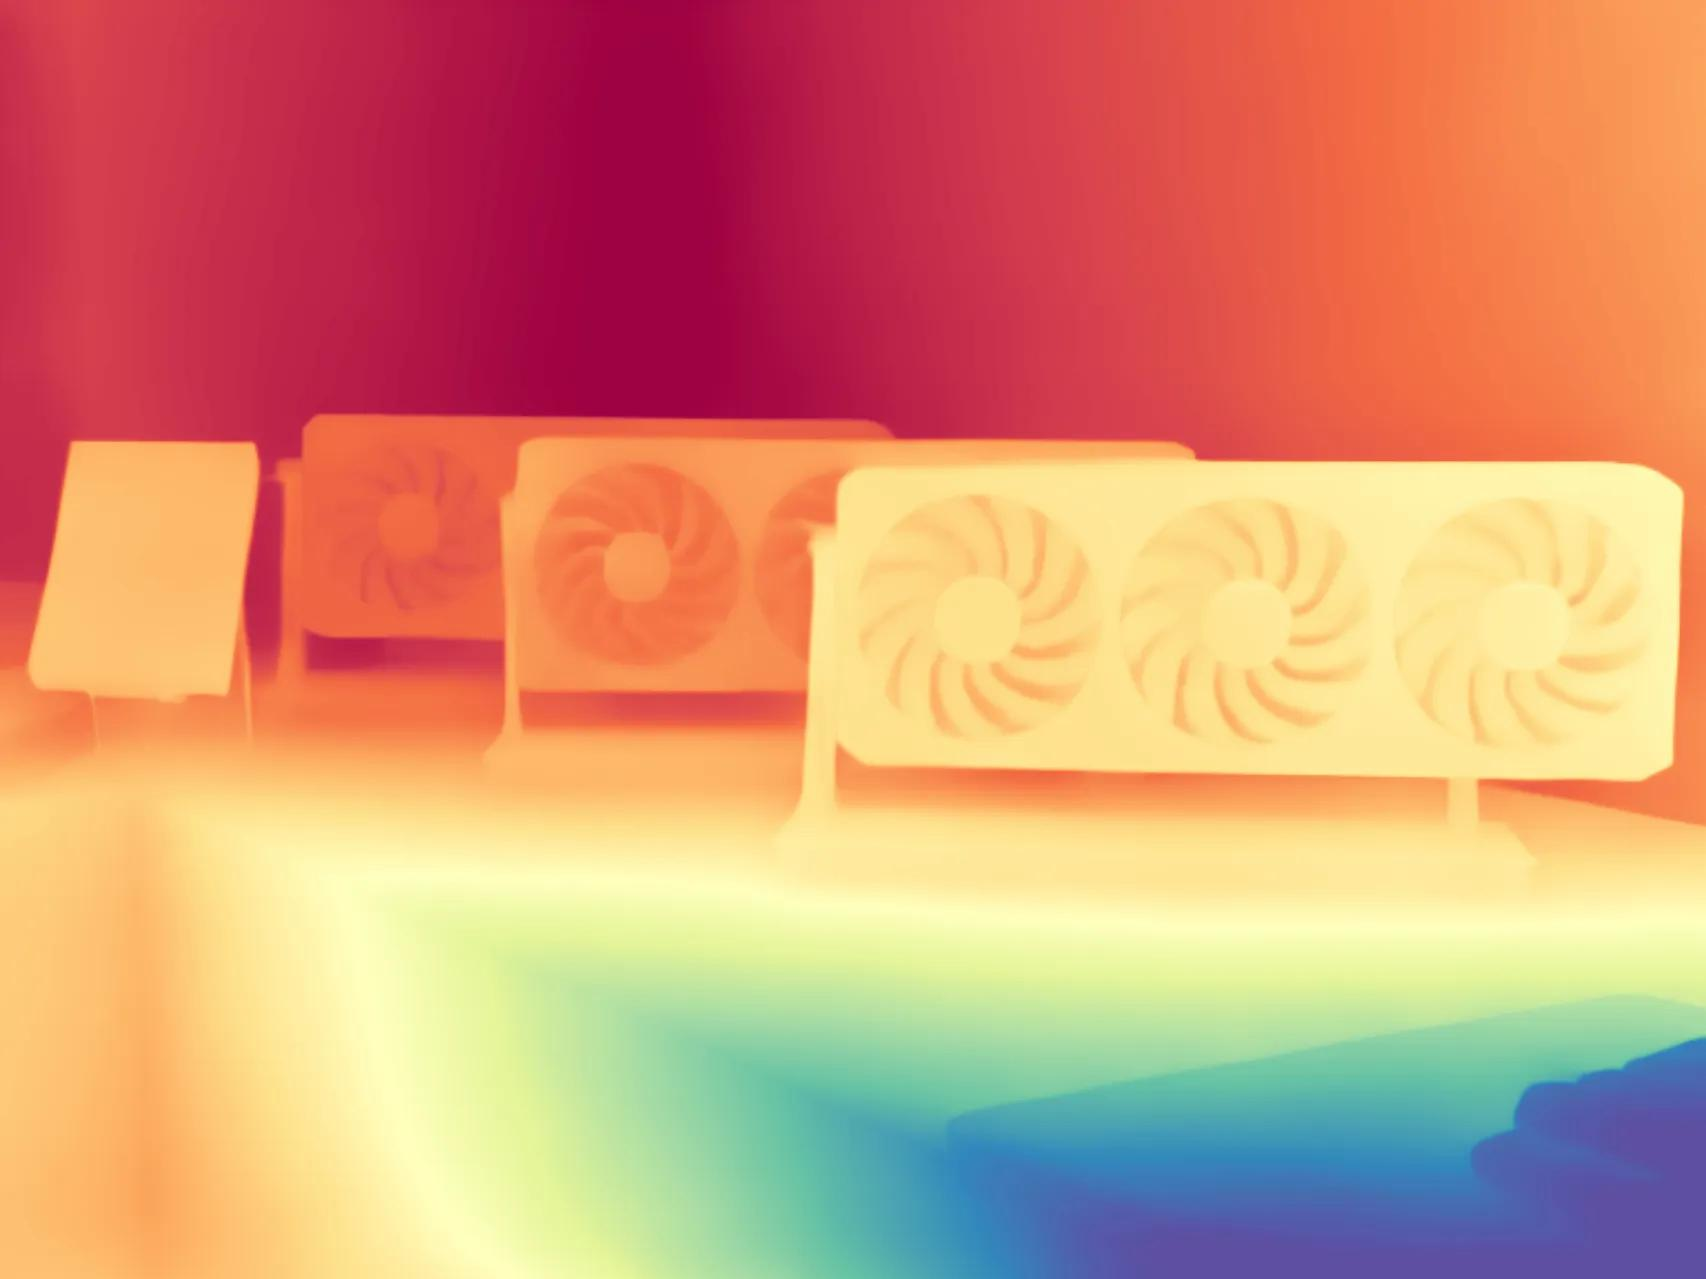
\includegraphics[width=0.22\textwidth]{images/depthmaster/inside-01_pred_colored.jpg} \\

    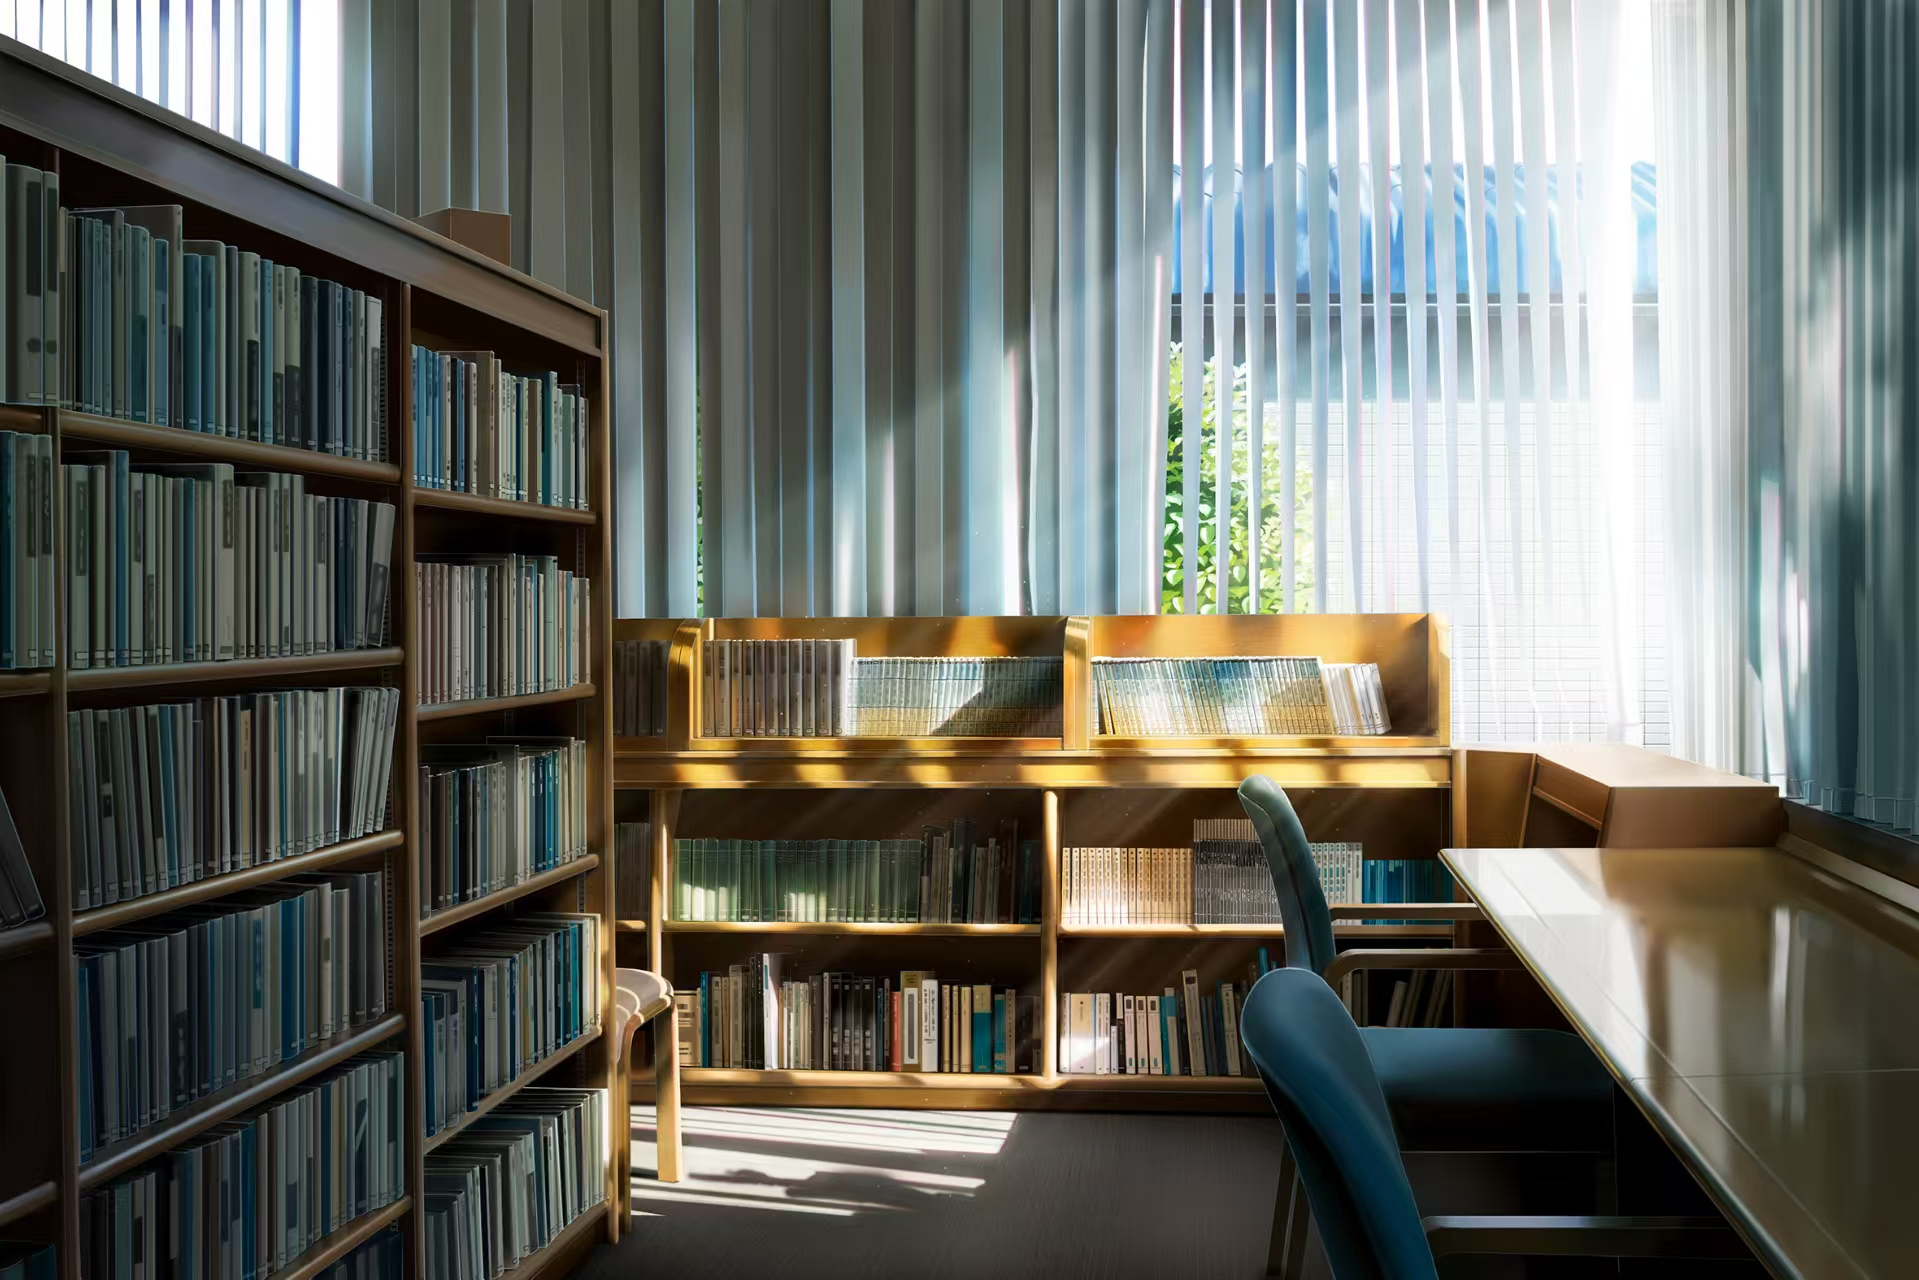
\includegraphics[width=0.22\textwidth]{images/test-image/synthetic-inside-01.jpg} &
    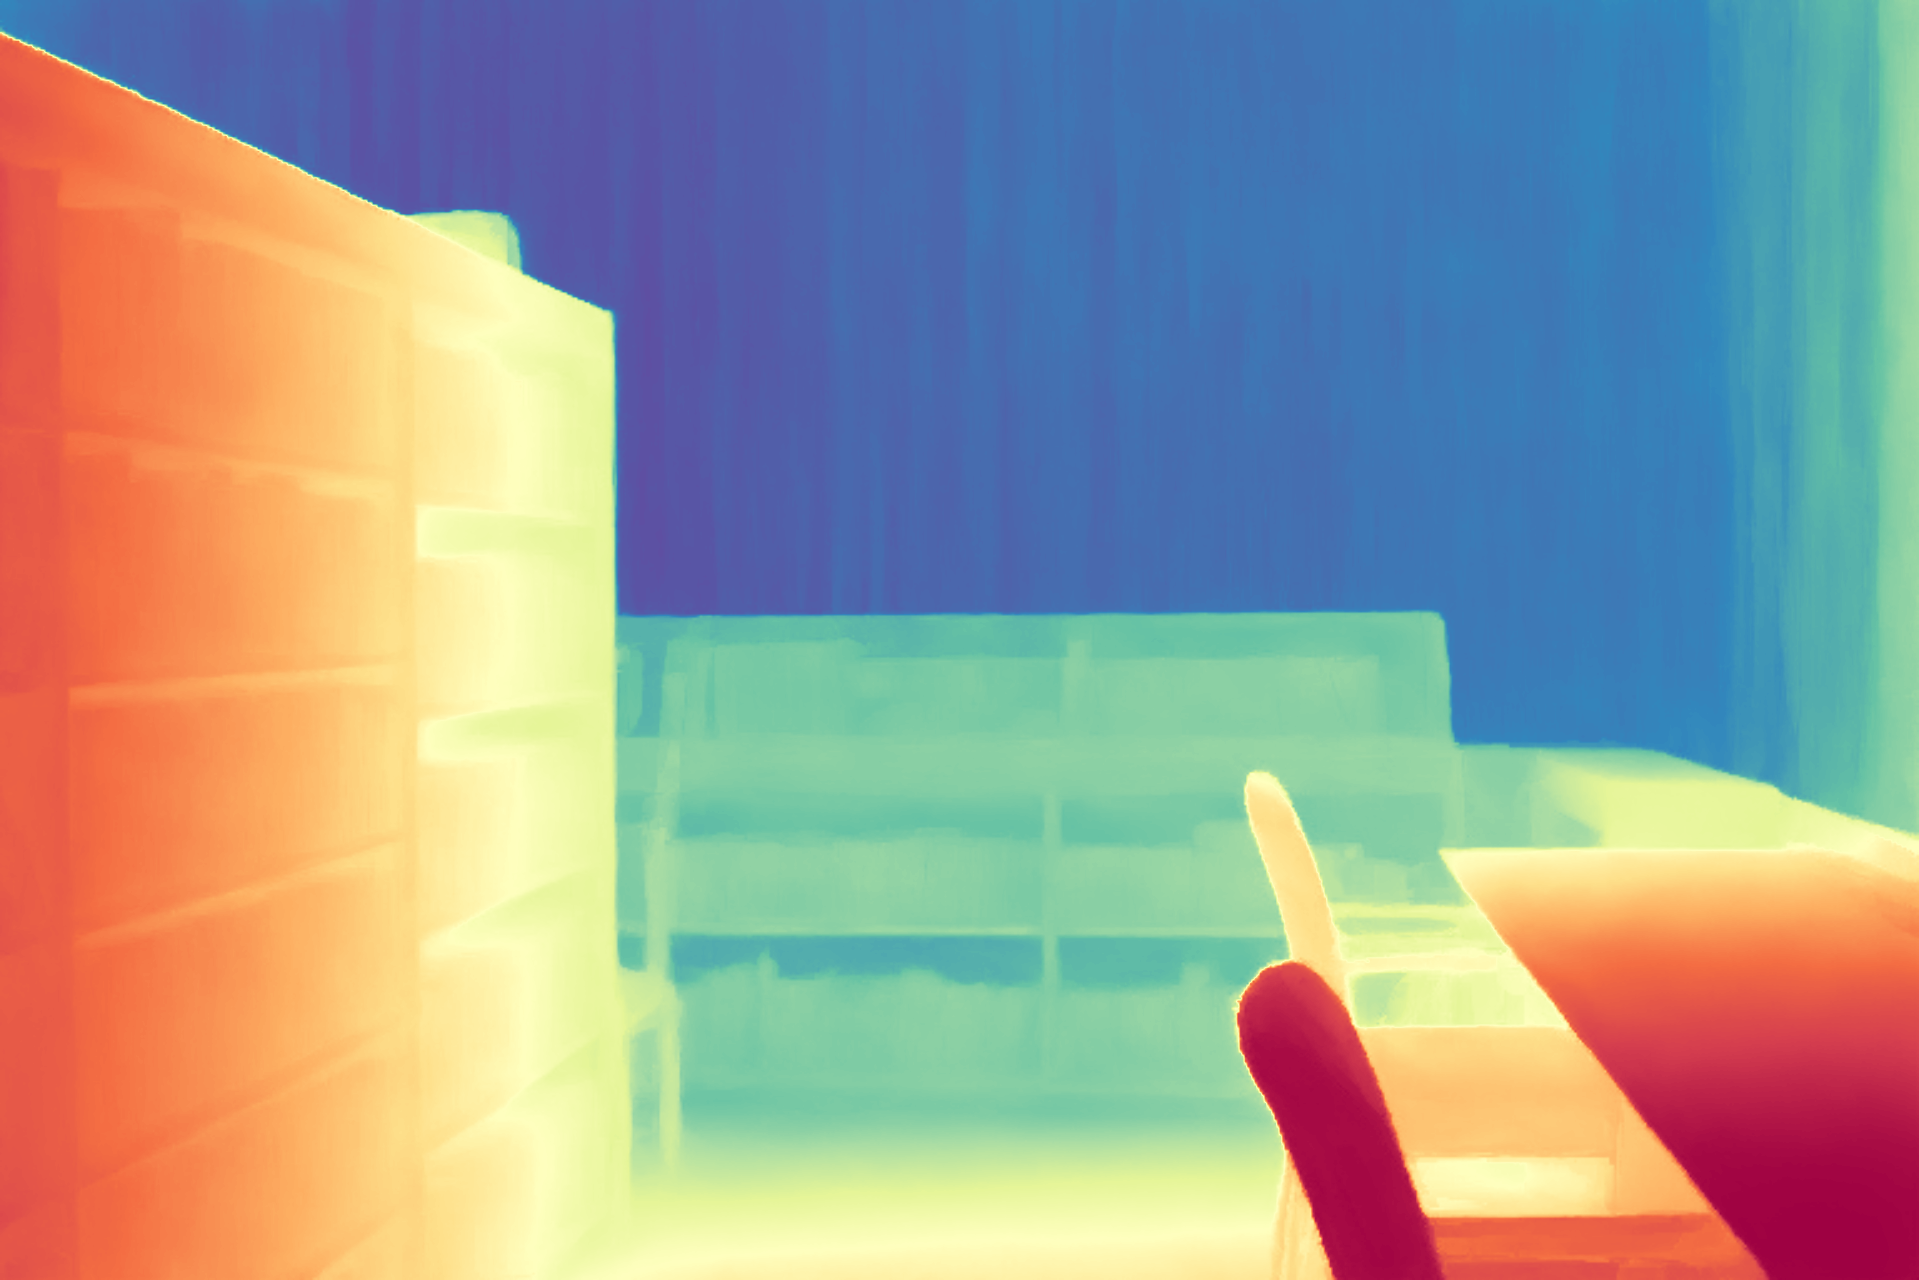
\includegraphics[width=0.22\textwidth]{images/trained/synthetic-inside-01_pred_colored.png} &
    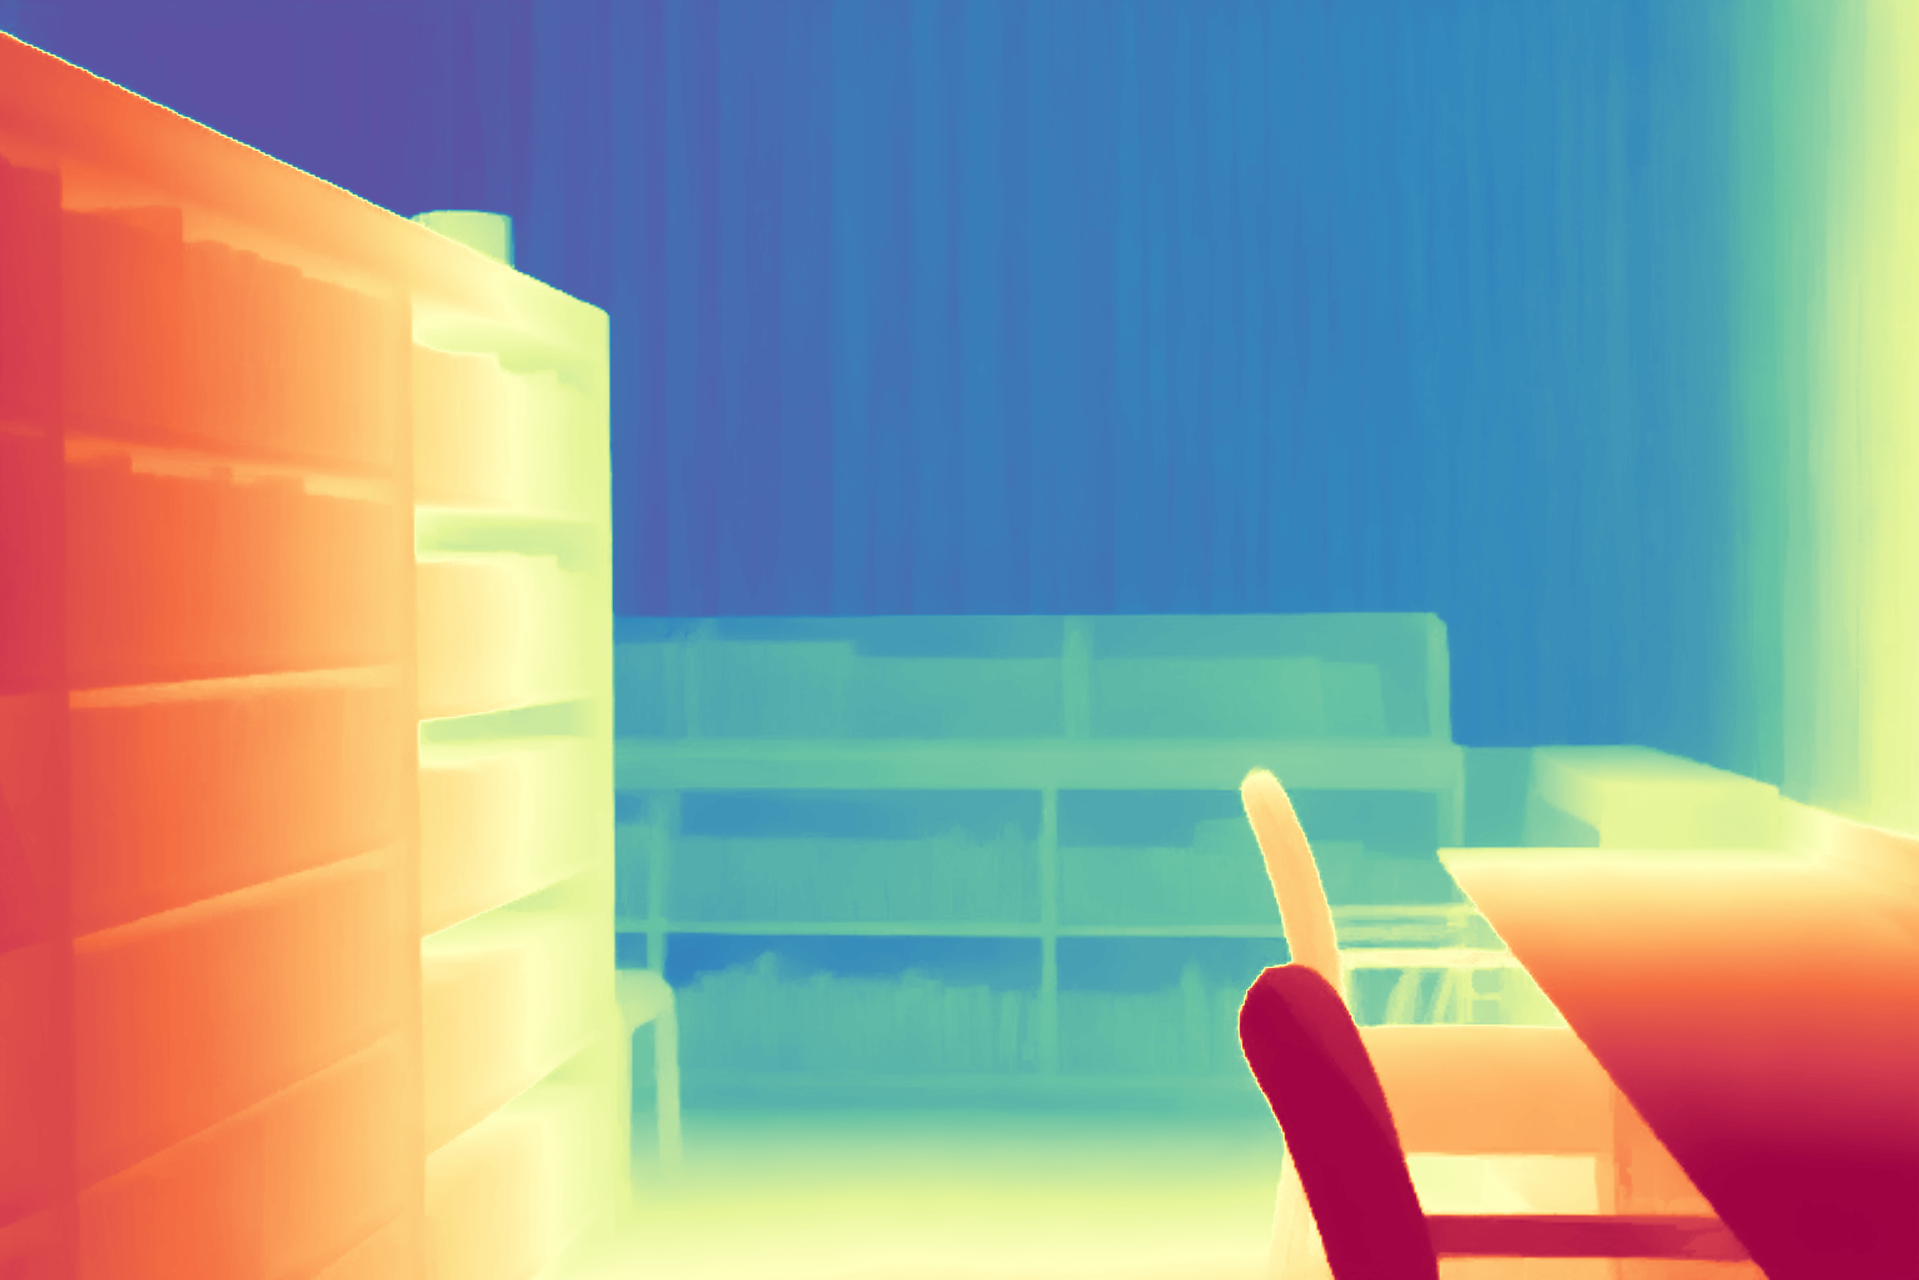
\includegraphics[width=0.22\textwidth]{images/pretrained/synthetic-inside-01_pred_colored.png} &
    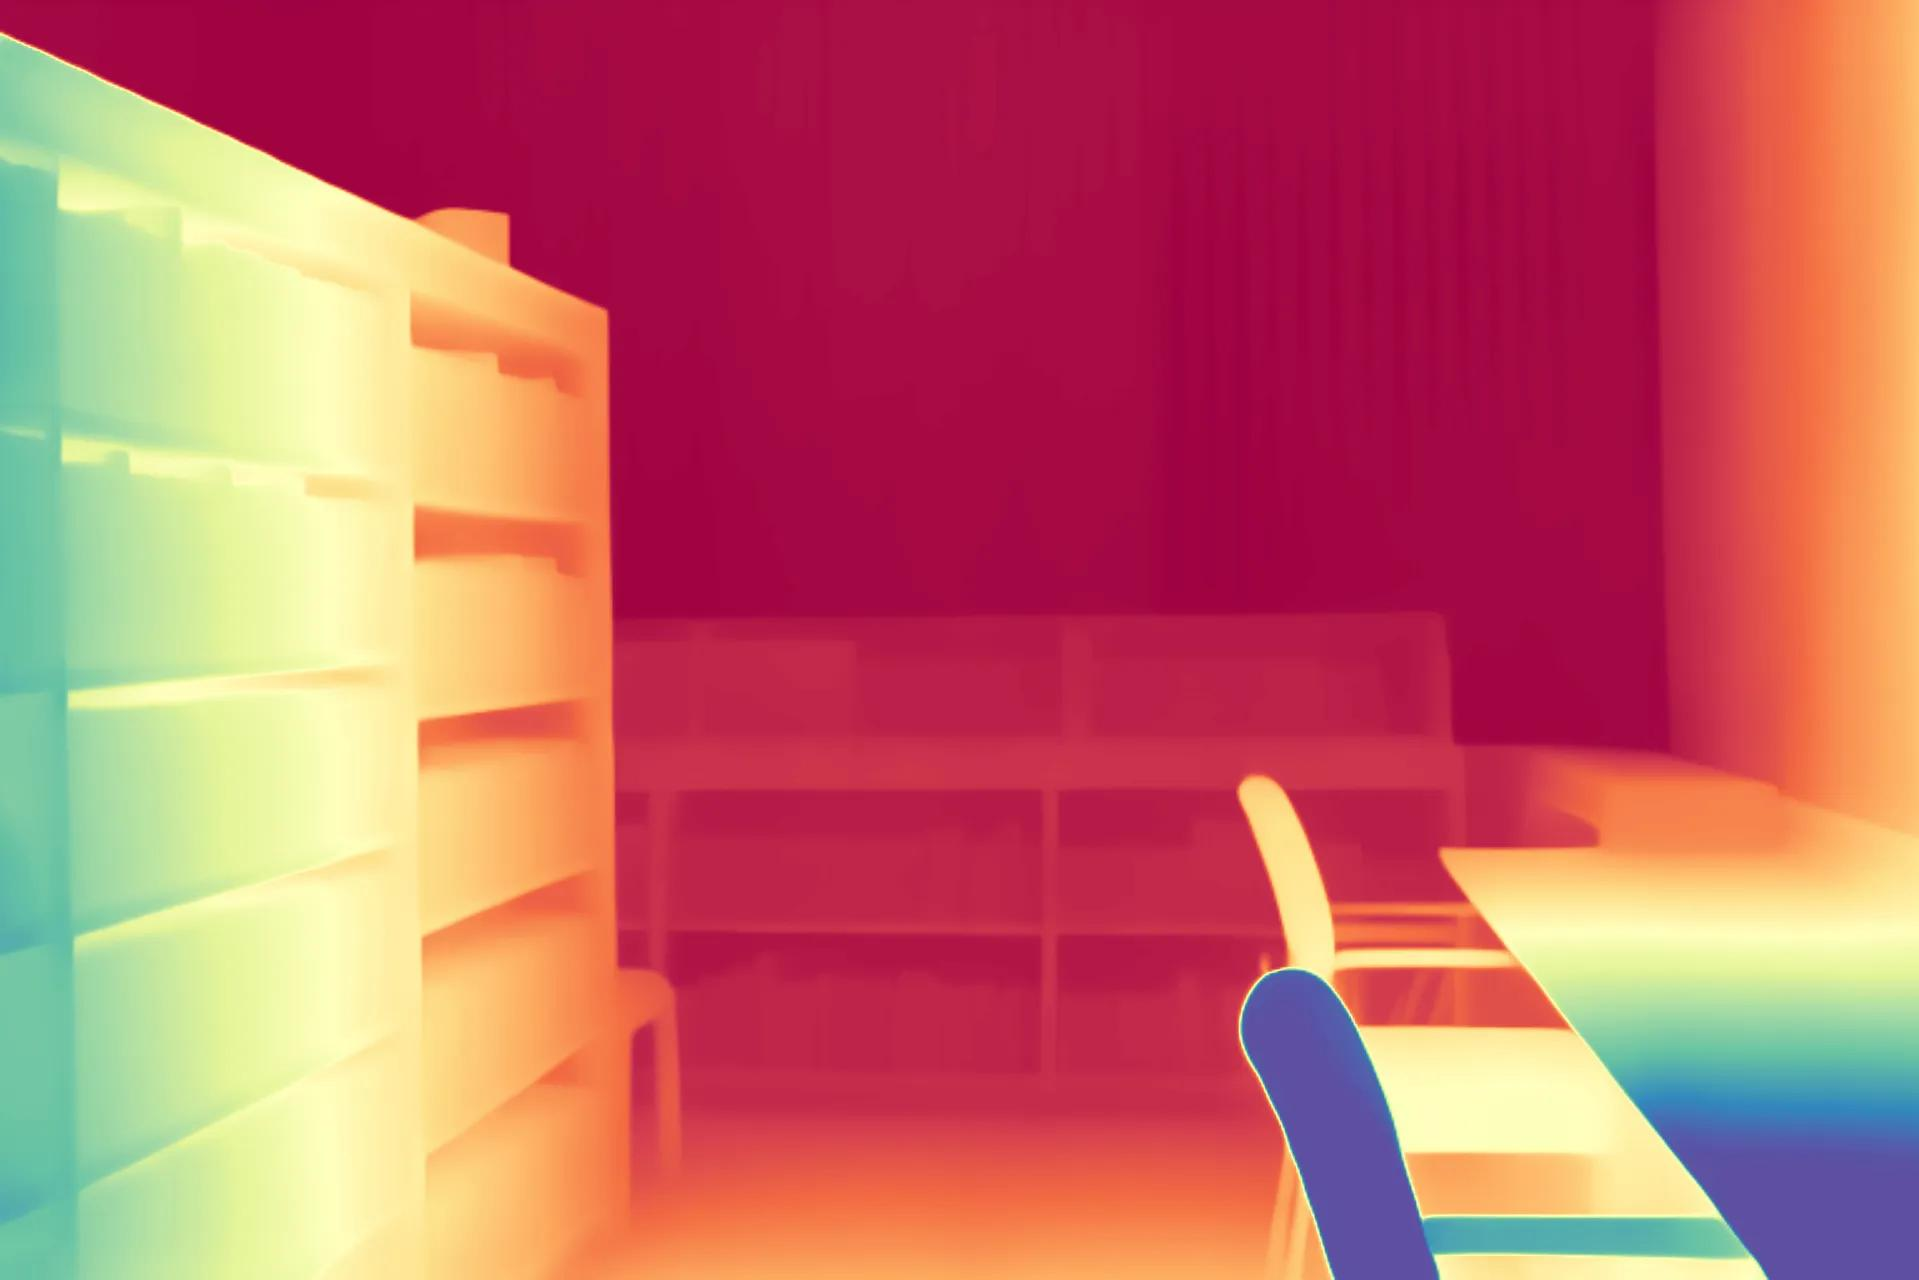
\includegraphics[width=0.22\textwidth]{images/depthmaster/synthetic-inside-01_pred_colored.jpg} \\

    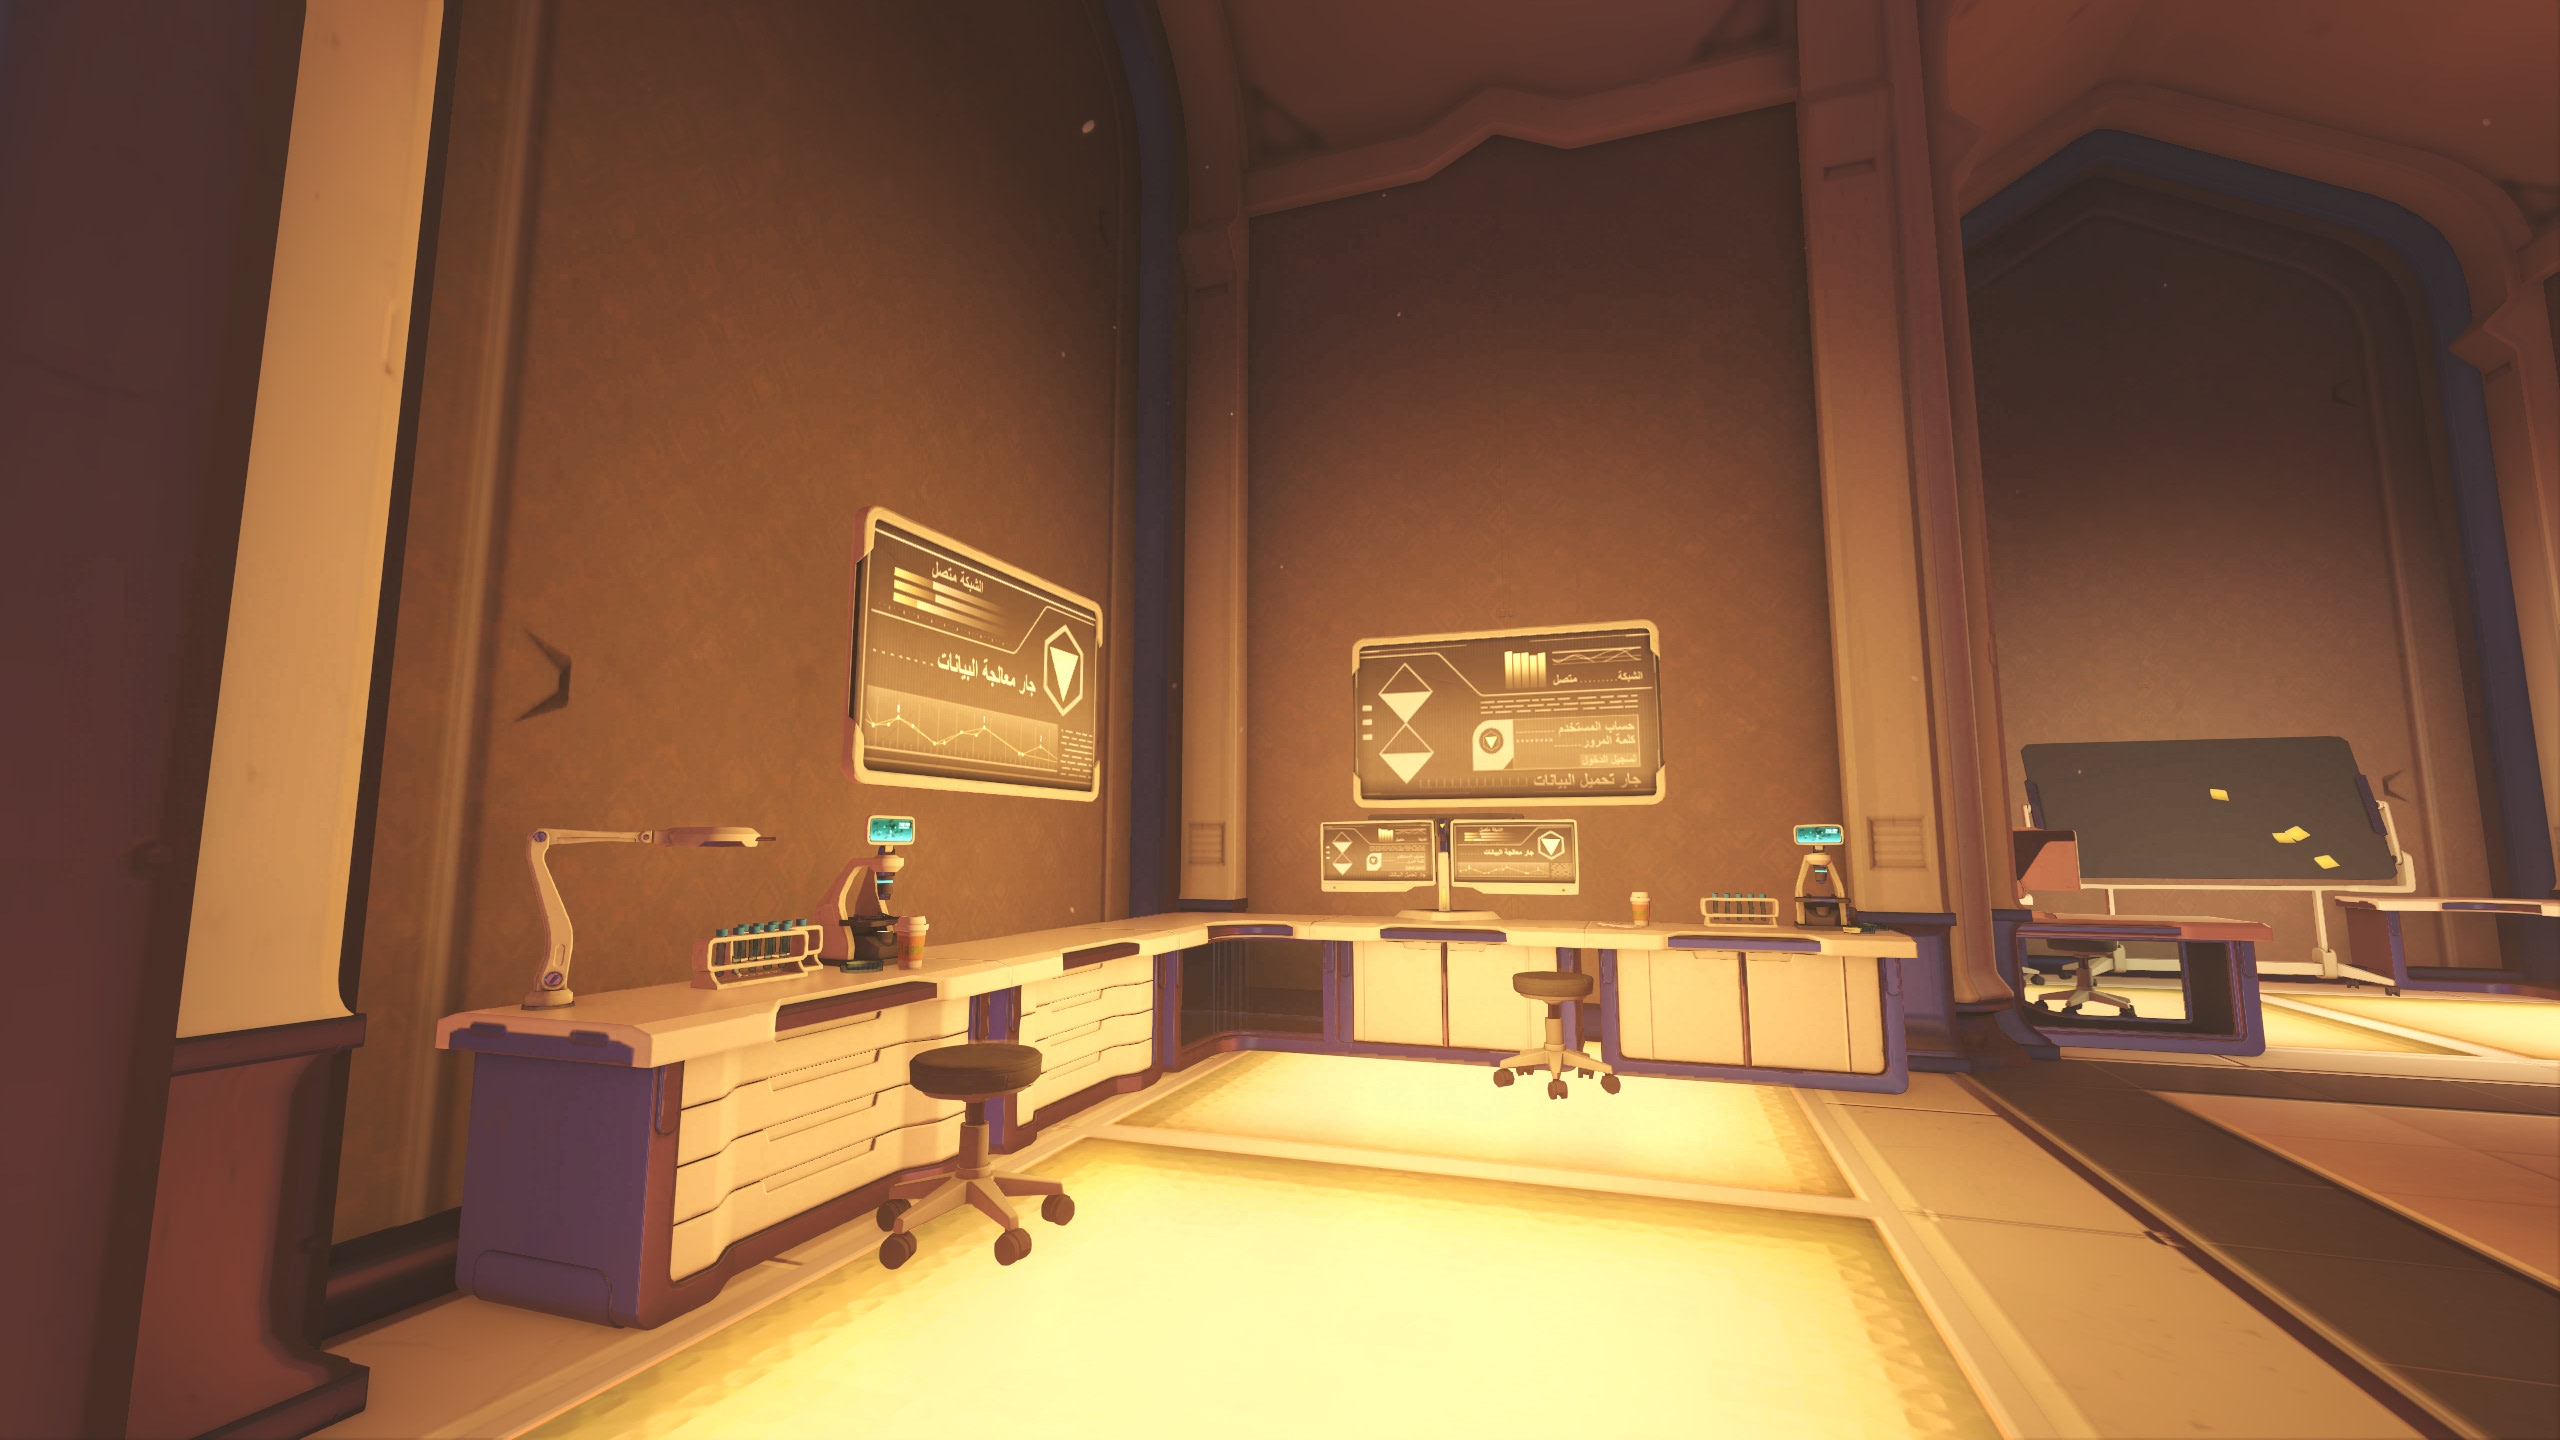
\includegraphics[width=0.22\textwidth]{images/test-image/synthetic-inside-02.jpg} &
    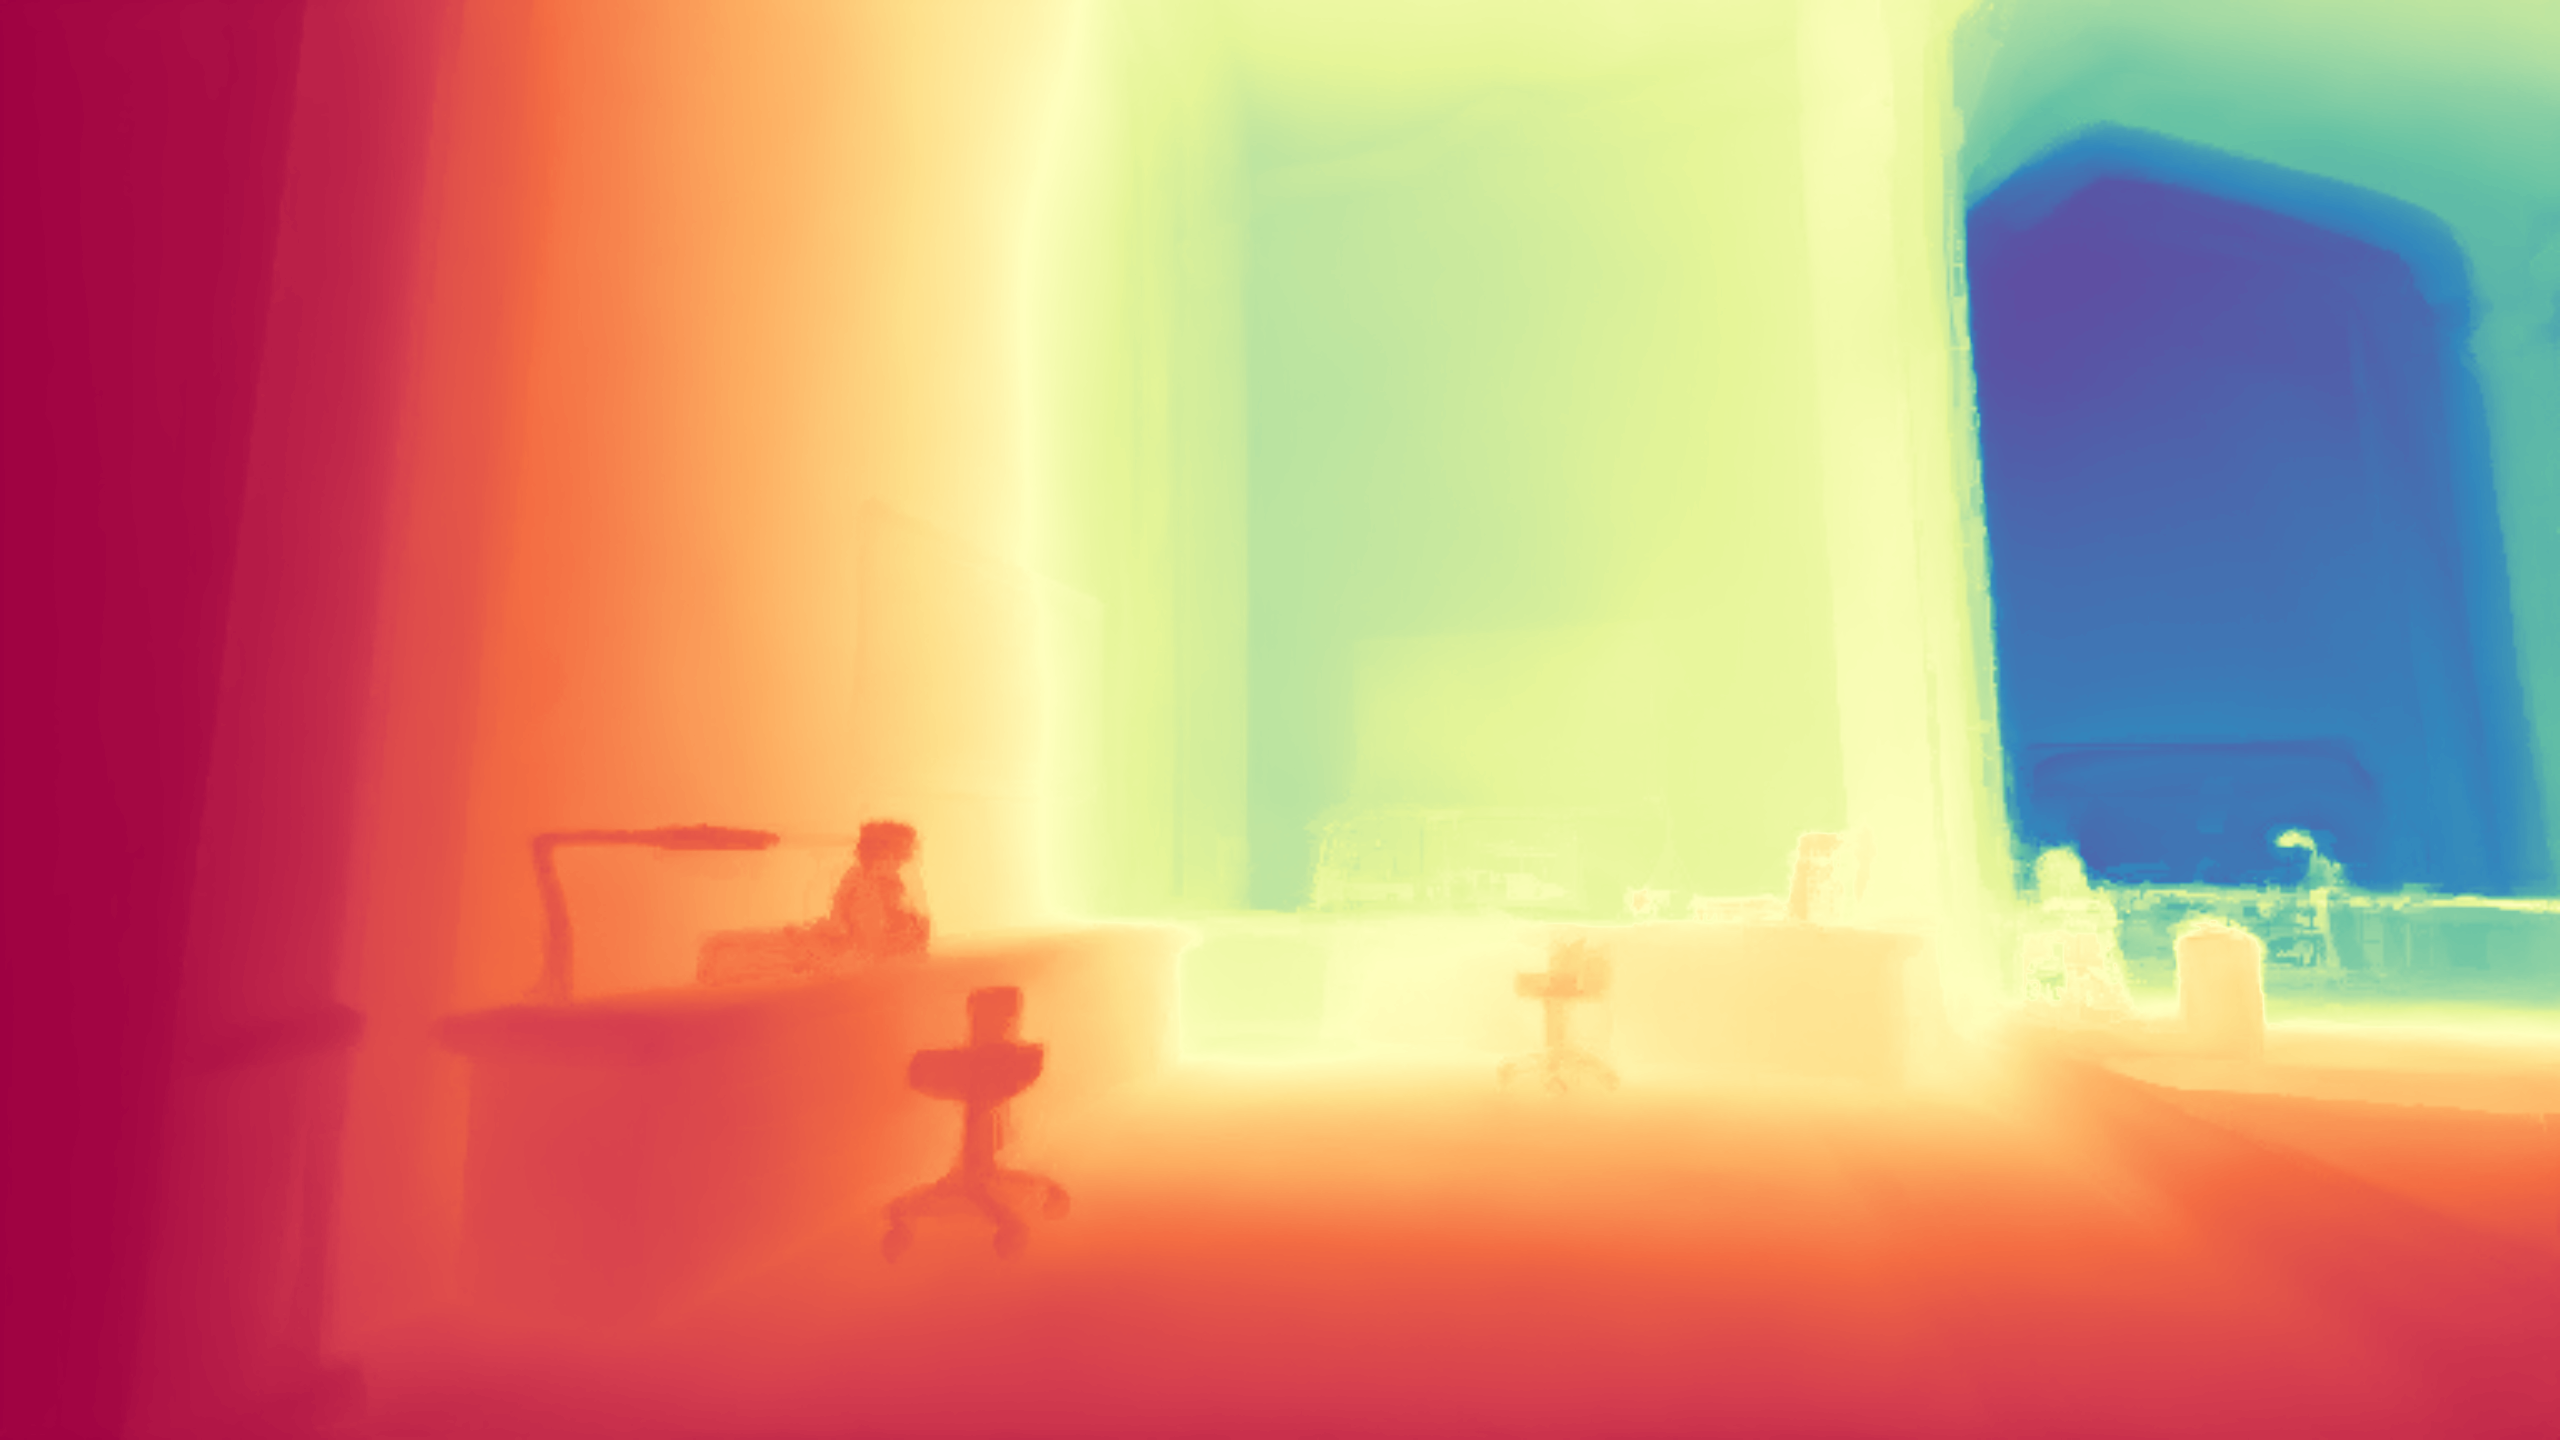
\includegraphics[width=0.22\textwidth]{images/trained/synthetic-inside-02_pred_colored.png} &
    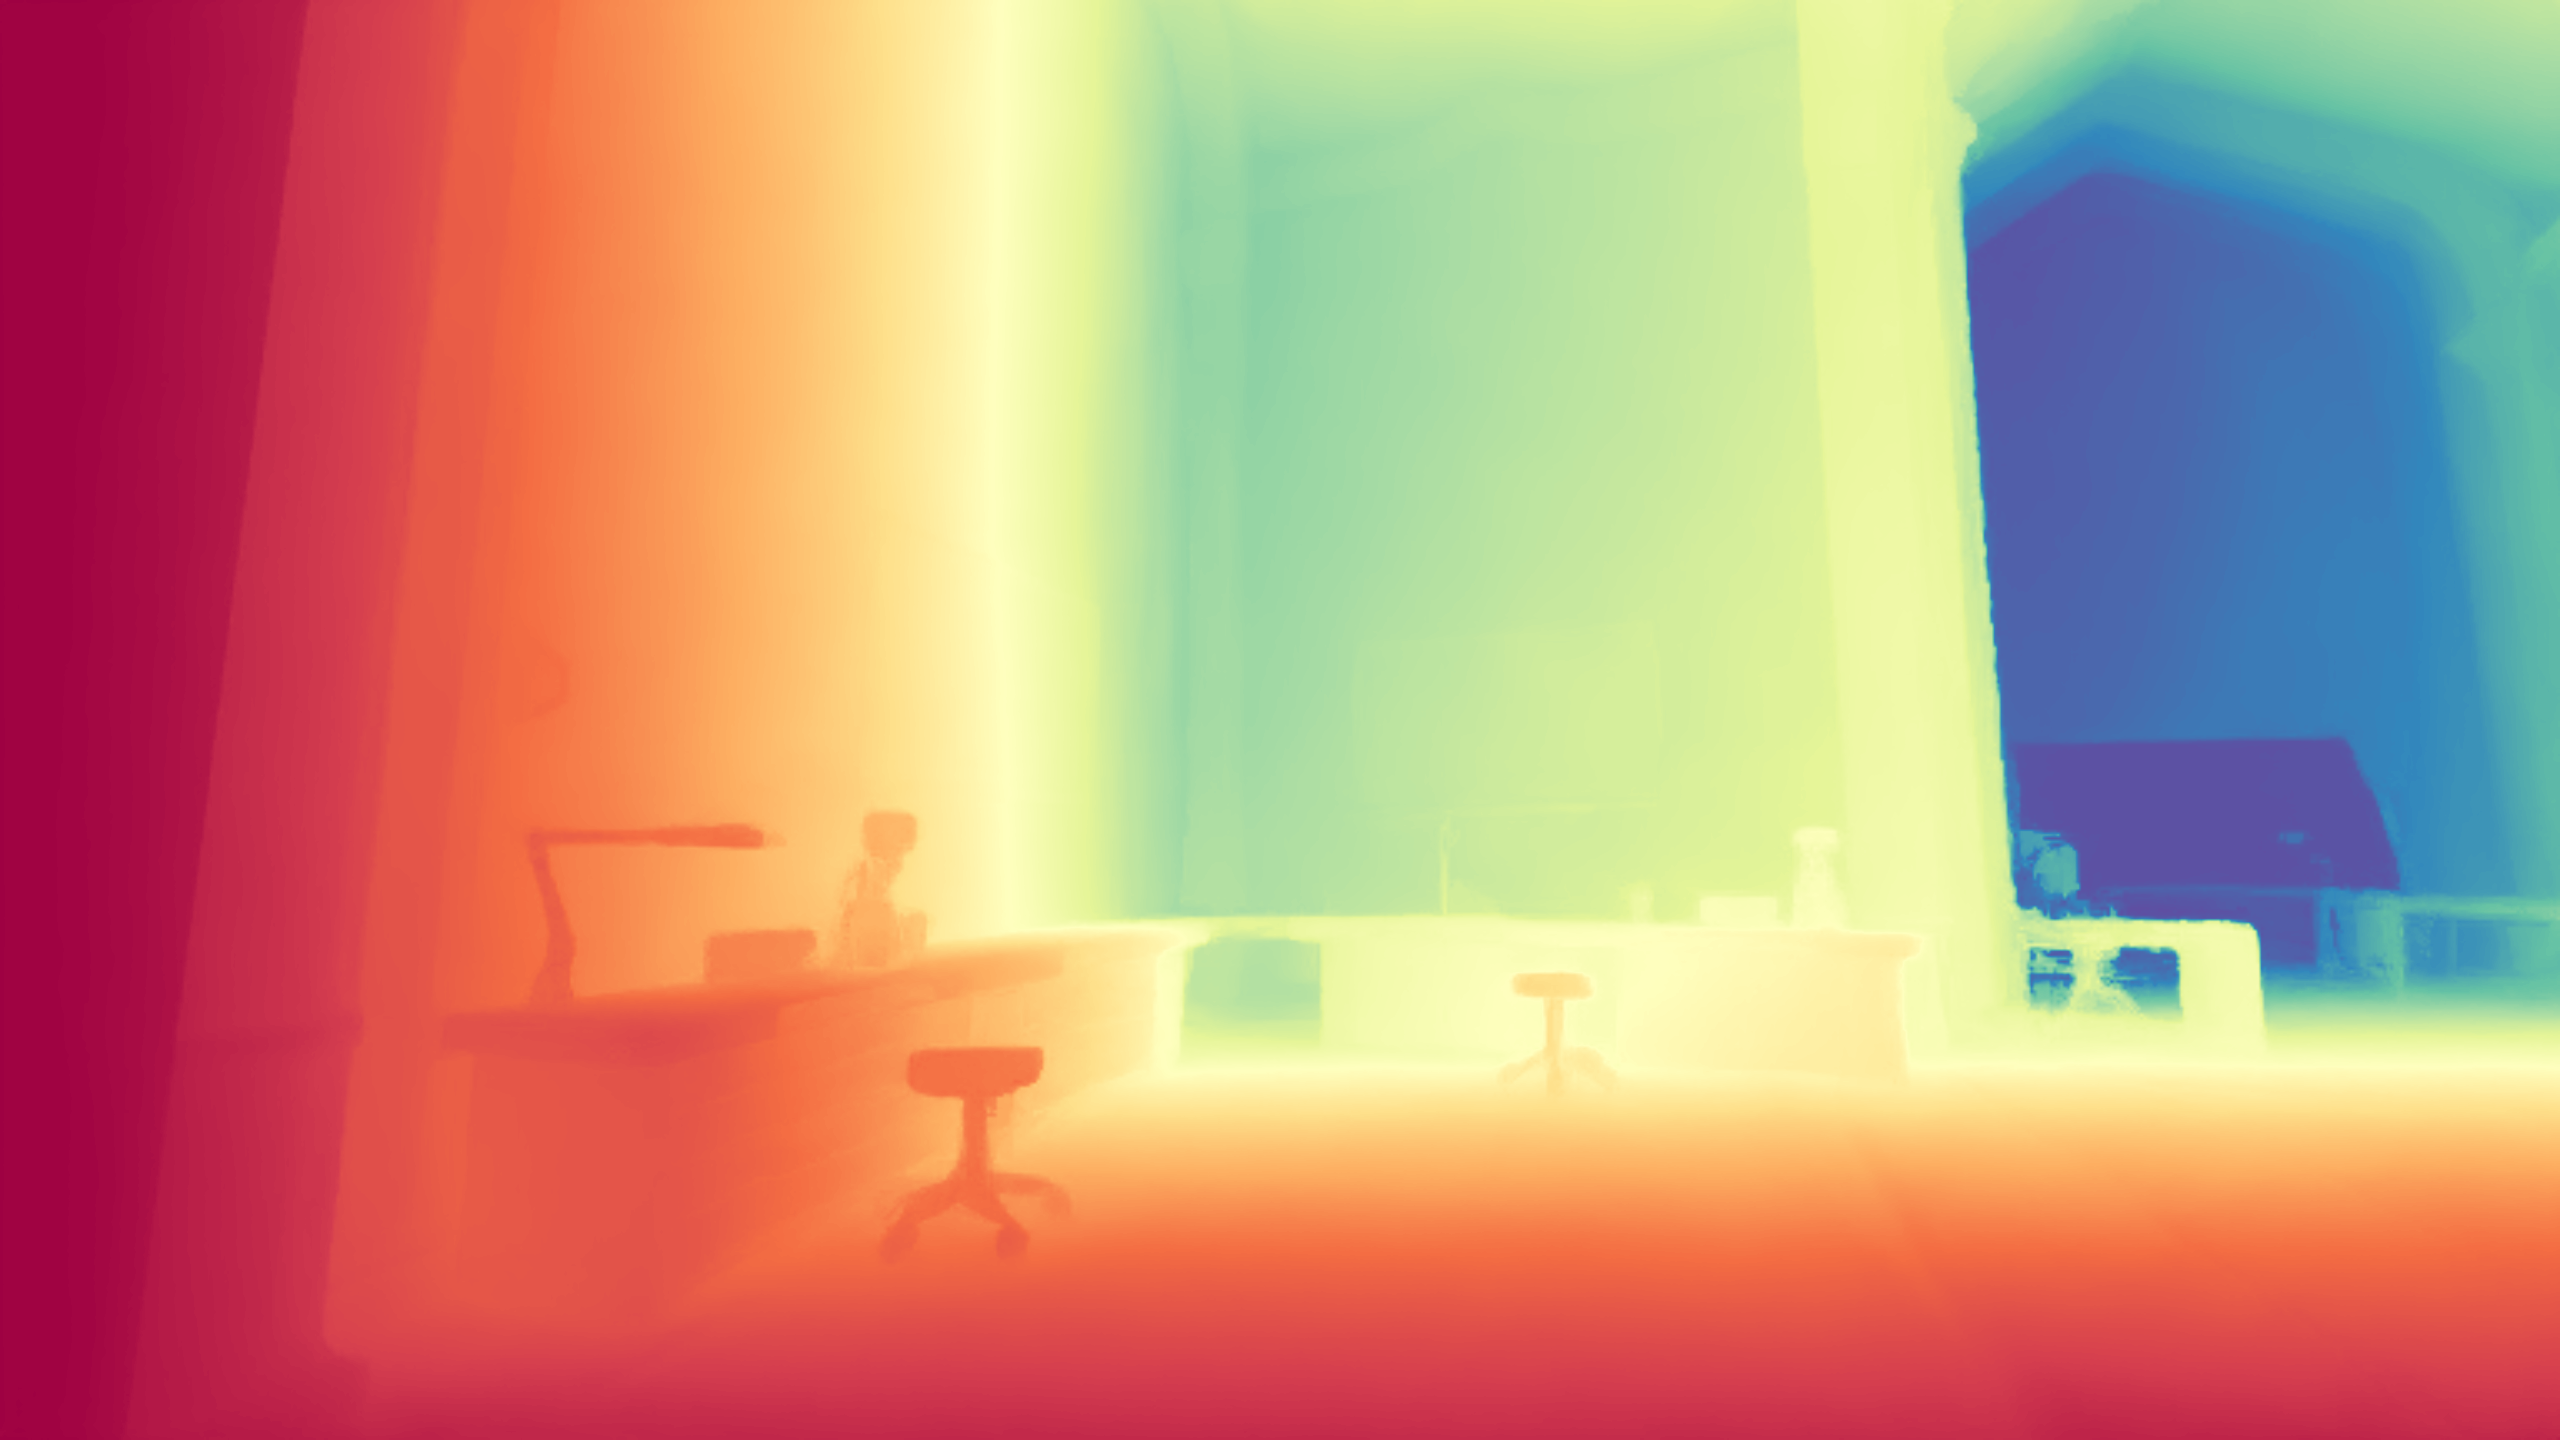
\includegraphics[width=0.22\textwidth]{images/pretrained/synthetic-inside-02_pred_colored.png} &
    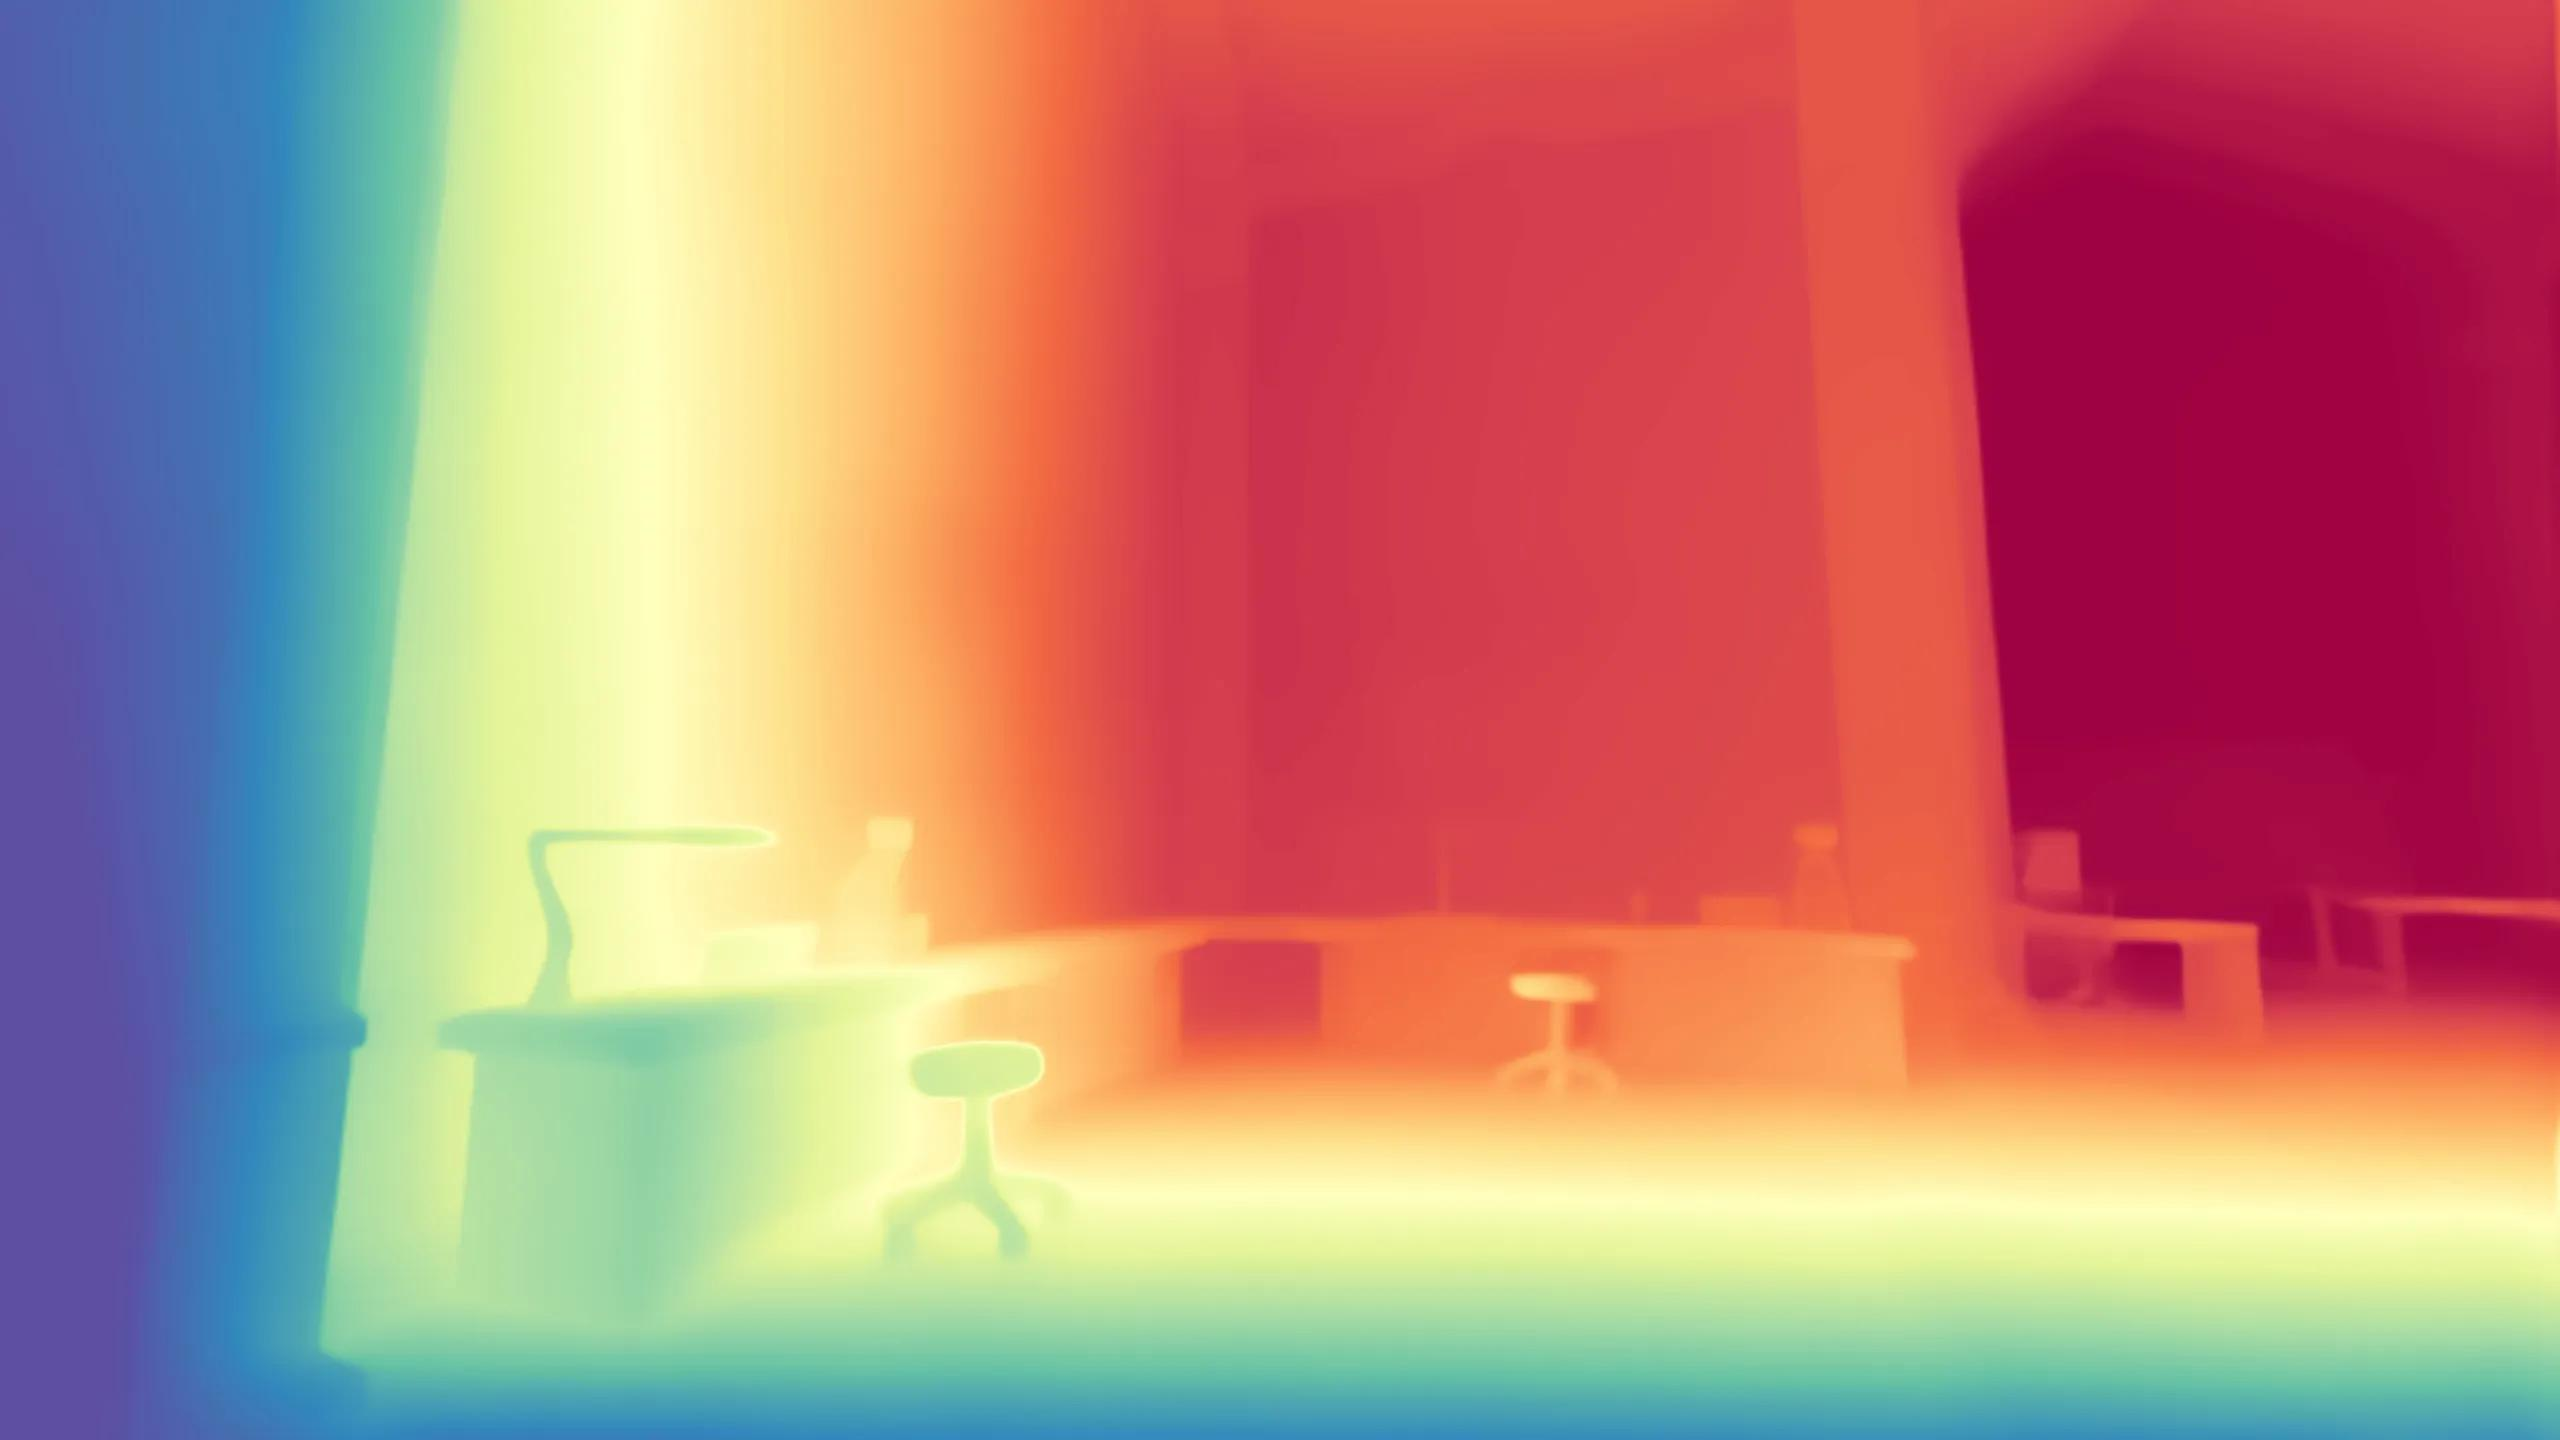
\includegraphics[width=0.22\textwidth]{images/depthmaster/synthetic-inside-02_pred_colored.jpg} \\

    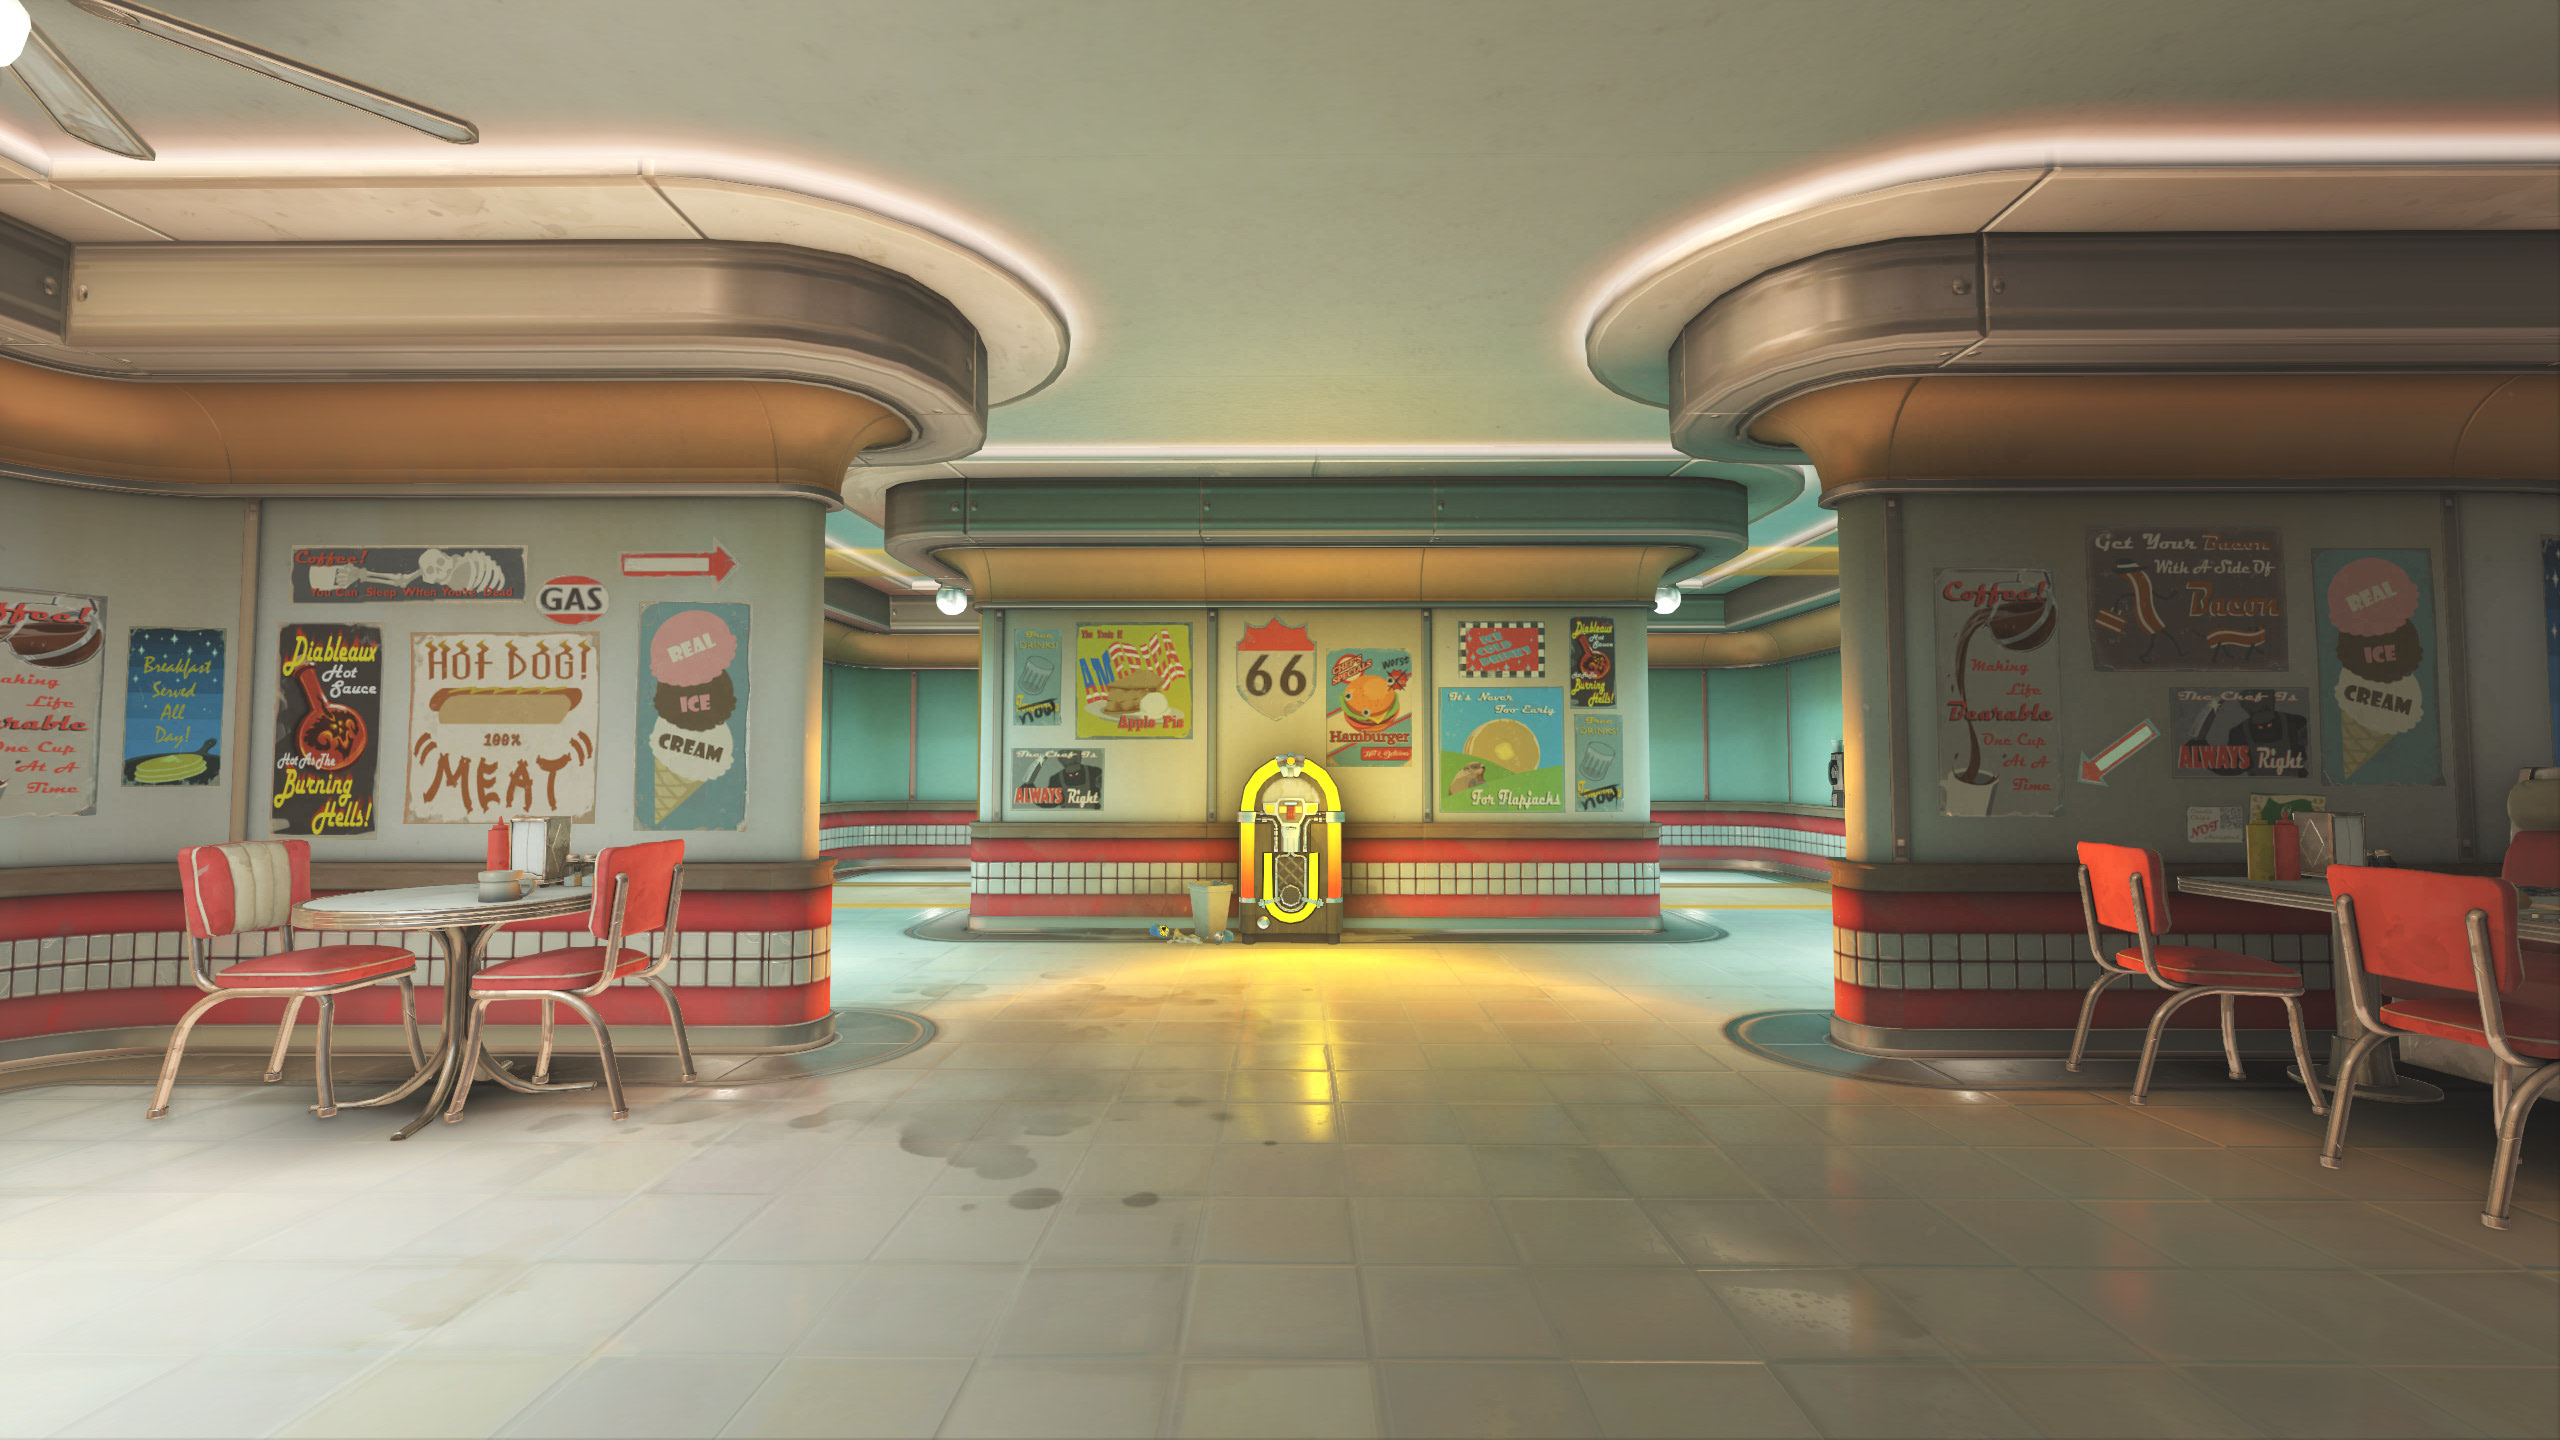
\includegraphics[width=0.22\textwidth]{images/test-image/synthetic-inside-03.jpg} &
    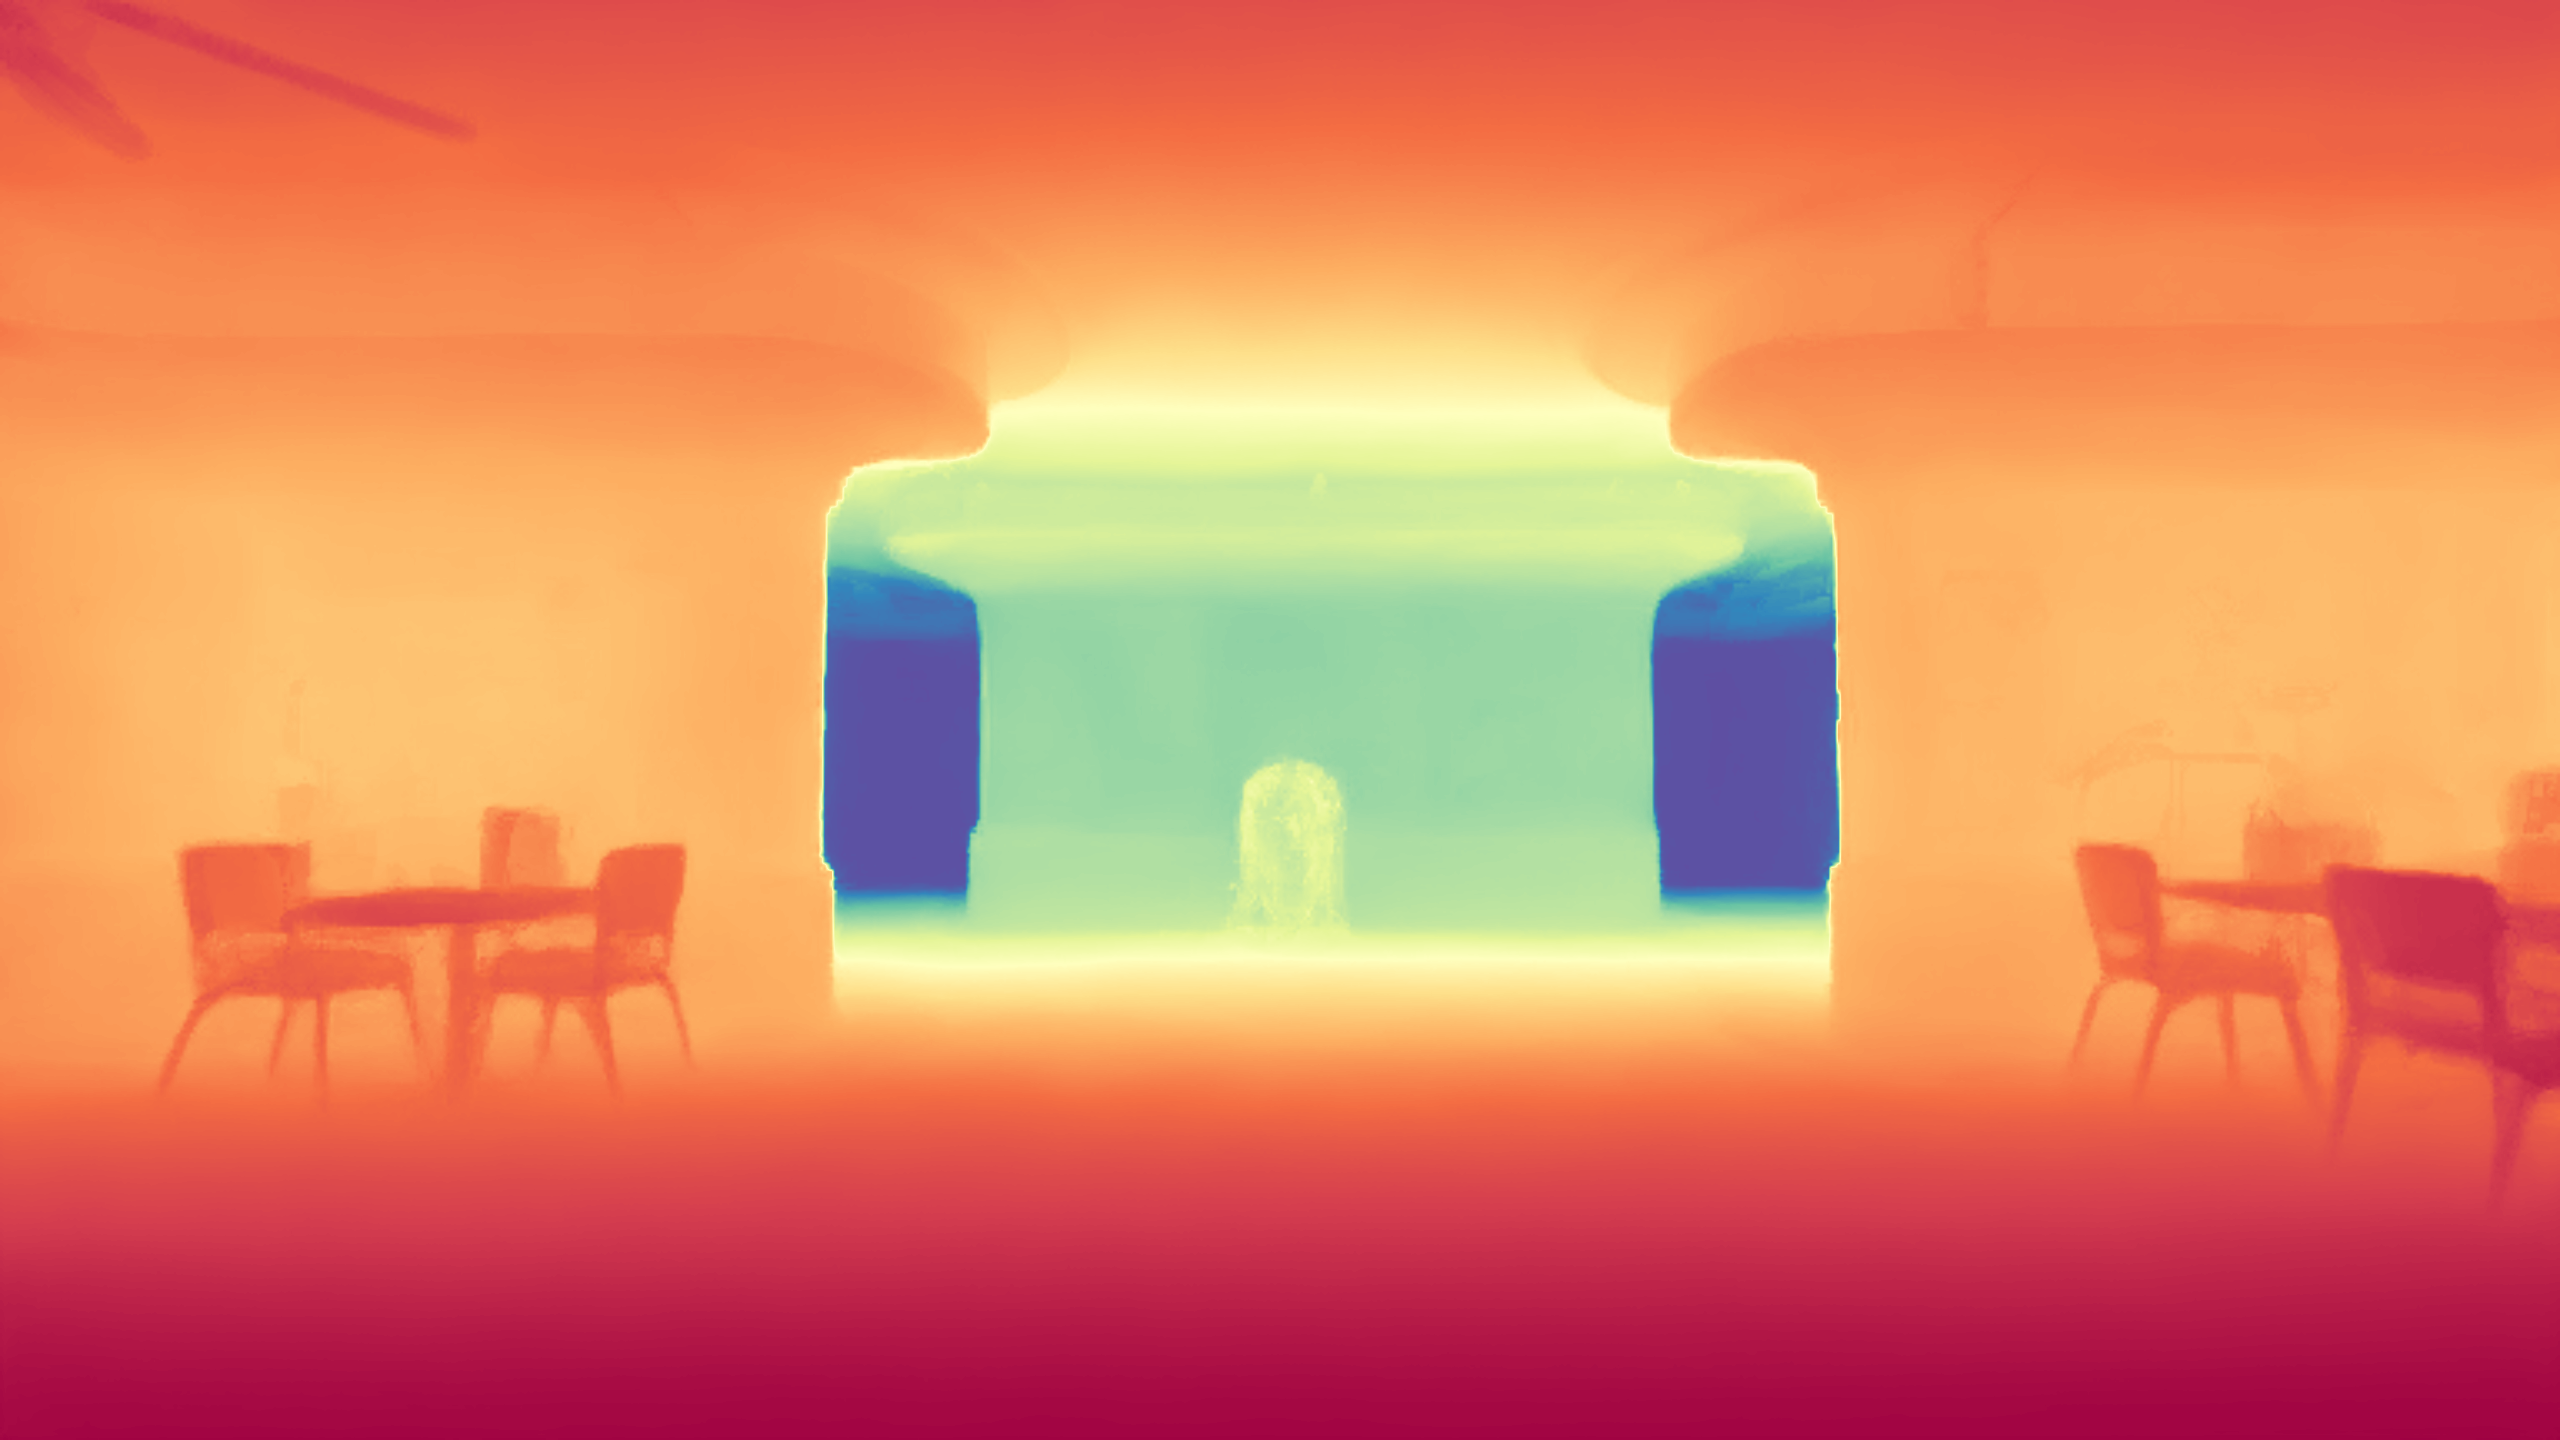
\includegraphics[width=0.22\textwidth]{images/trained/synthetic-inside-03_pred_colored.png} &
    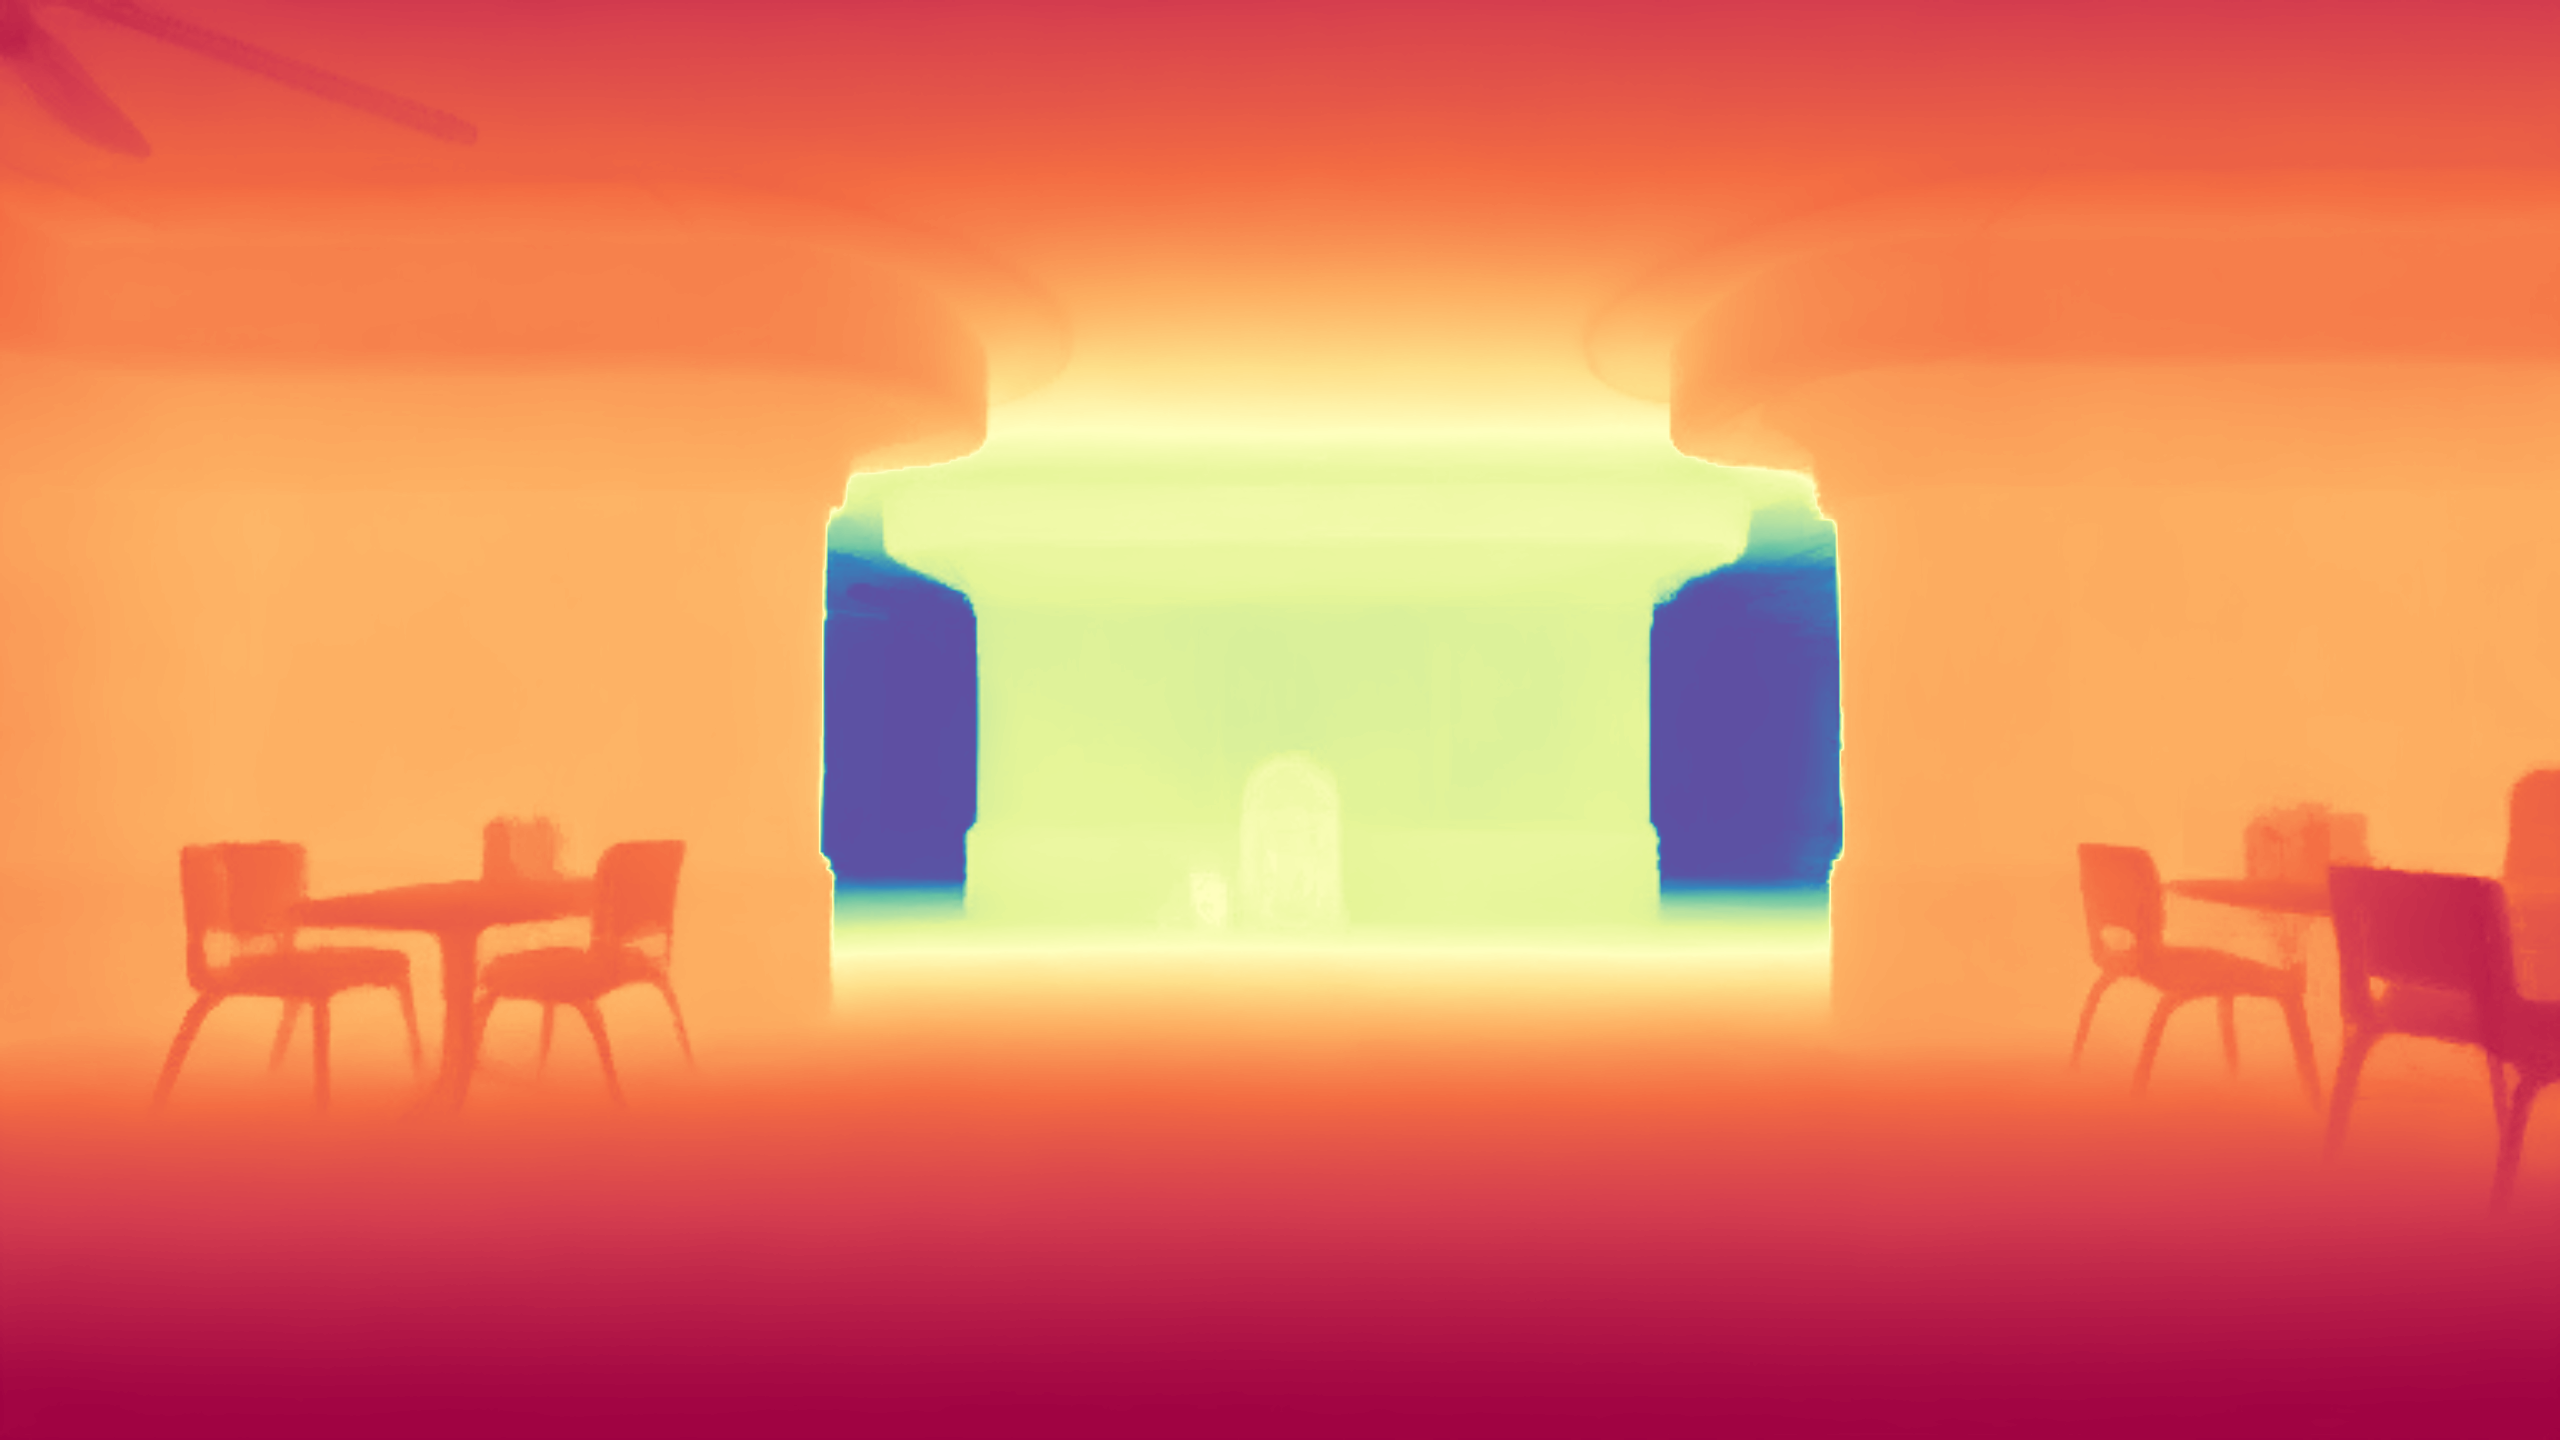
\includegraphics[width=0.22\textwidth]{images/pretrained/synthetic-inside-03_pred_colored.png} &
    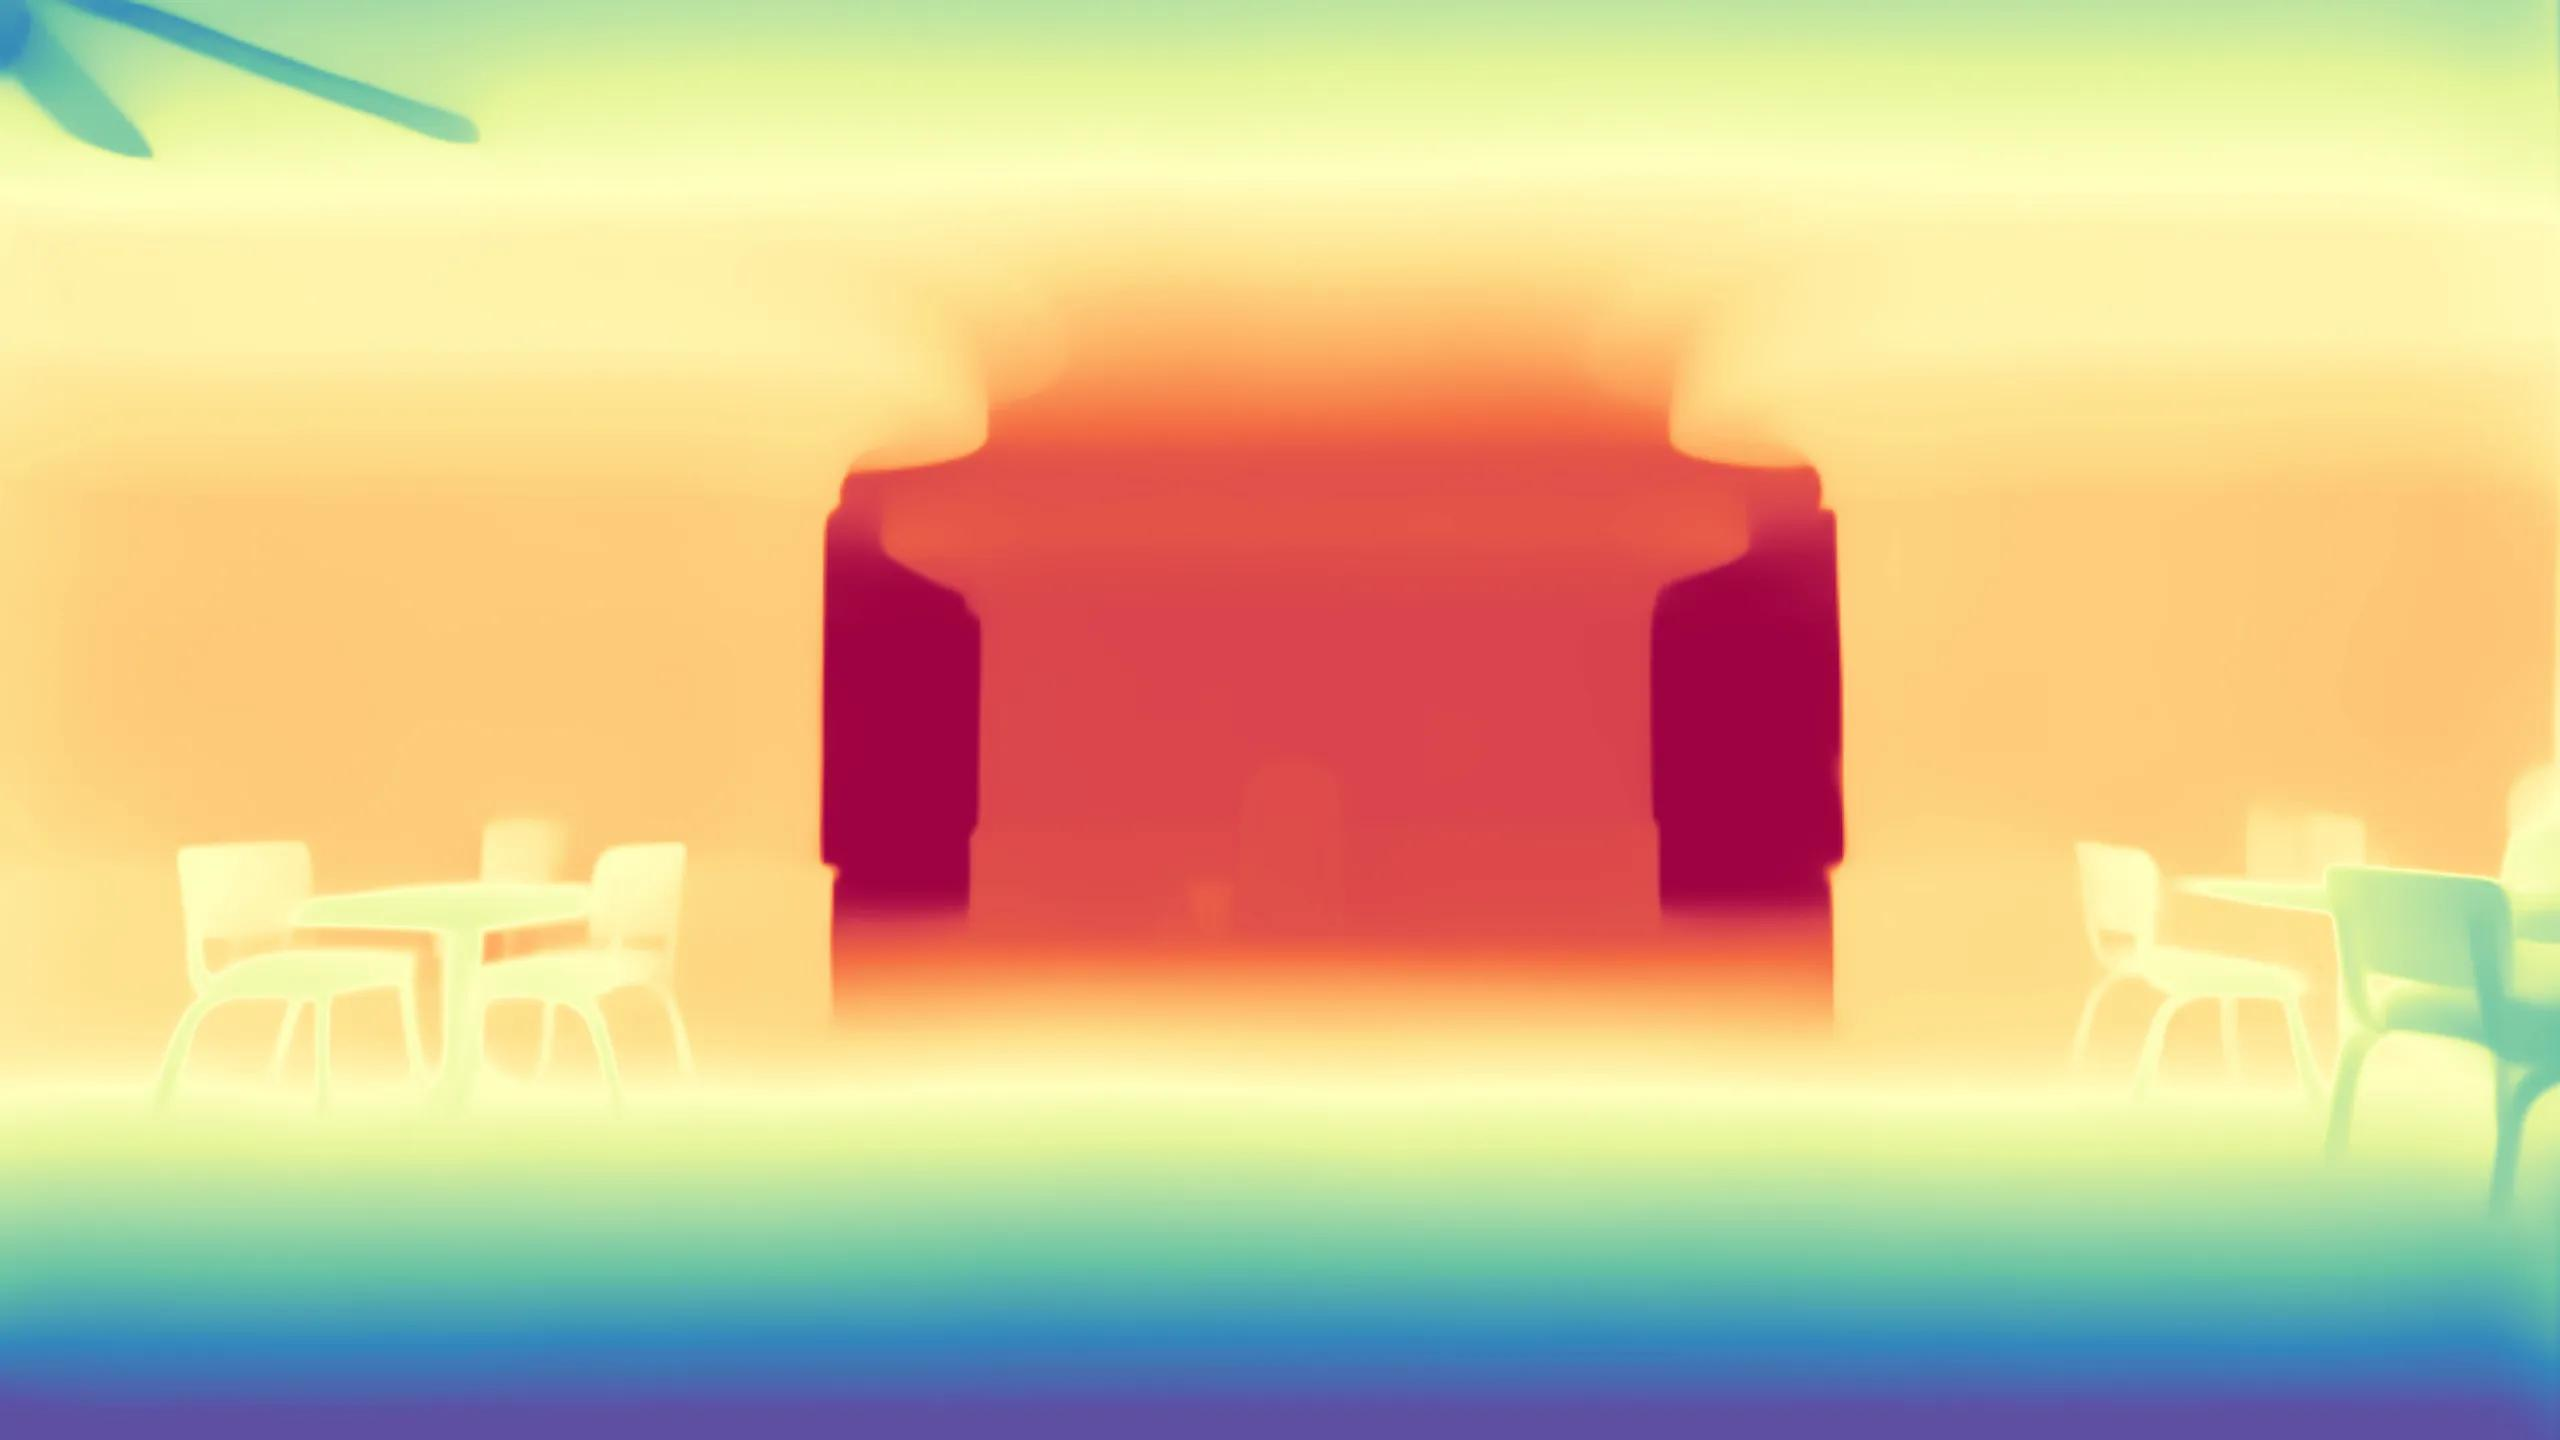
\includegraphics[width=0.22\textwidth]{images/depthmaster/synthetic-inside-03_pred_colored.jpg} \\

    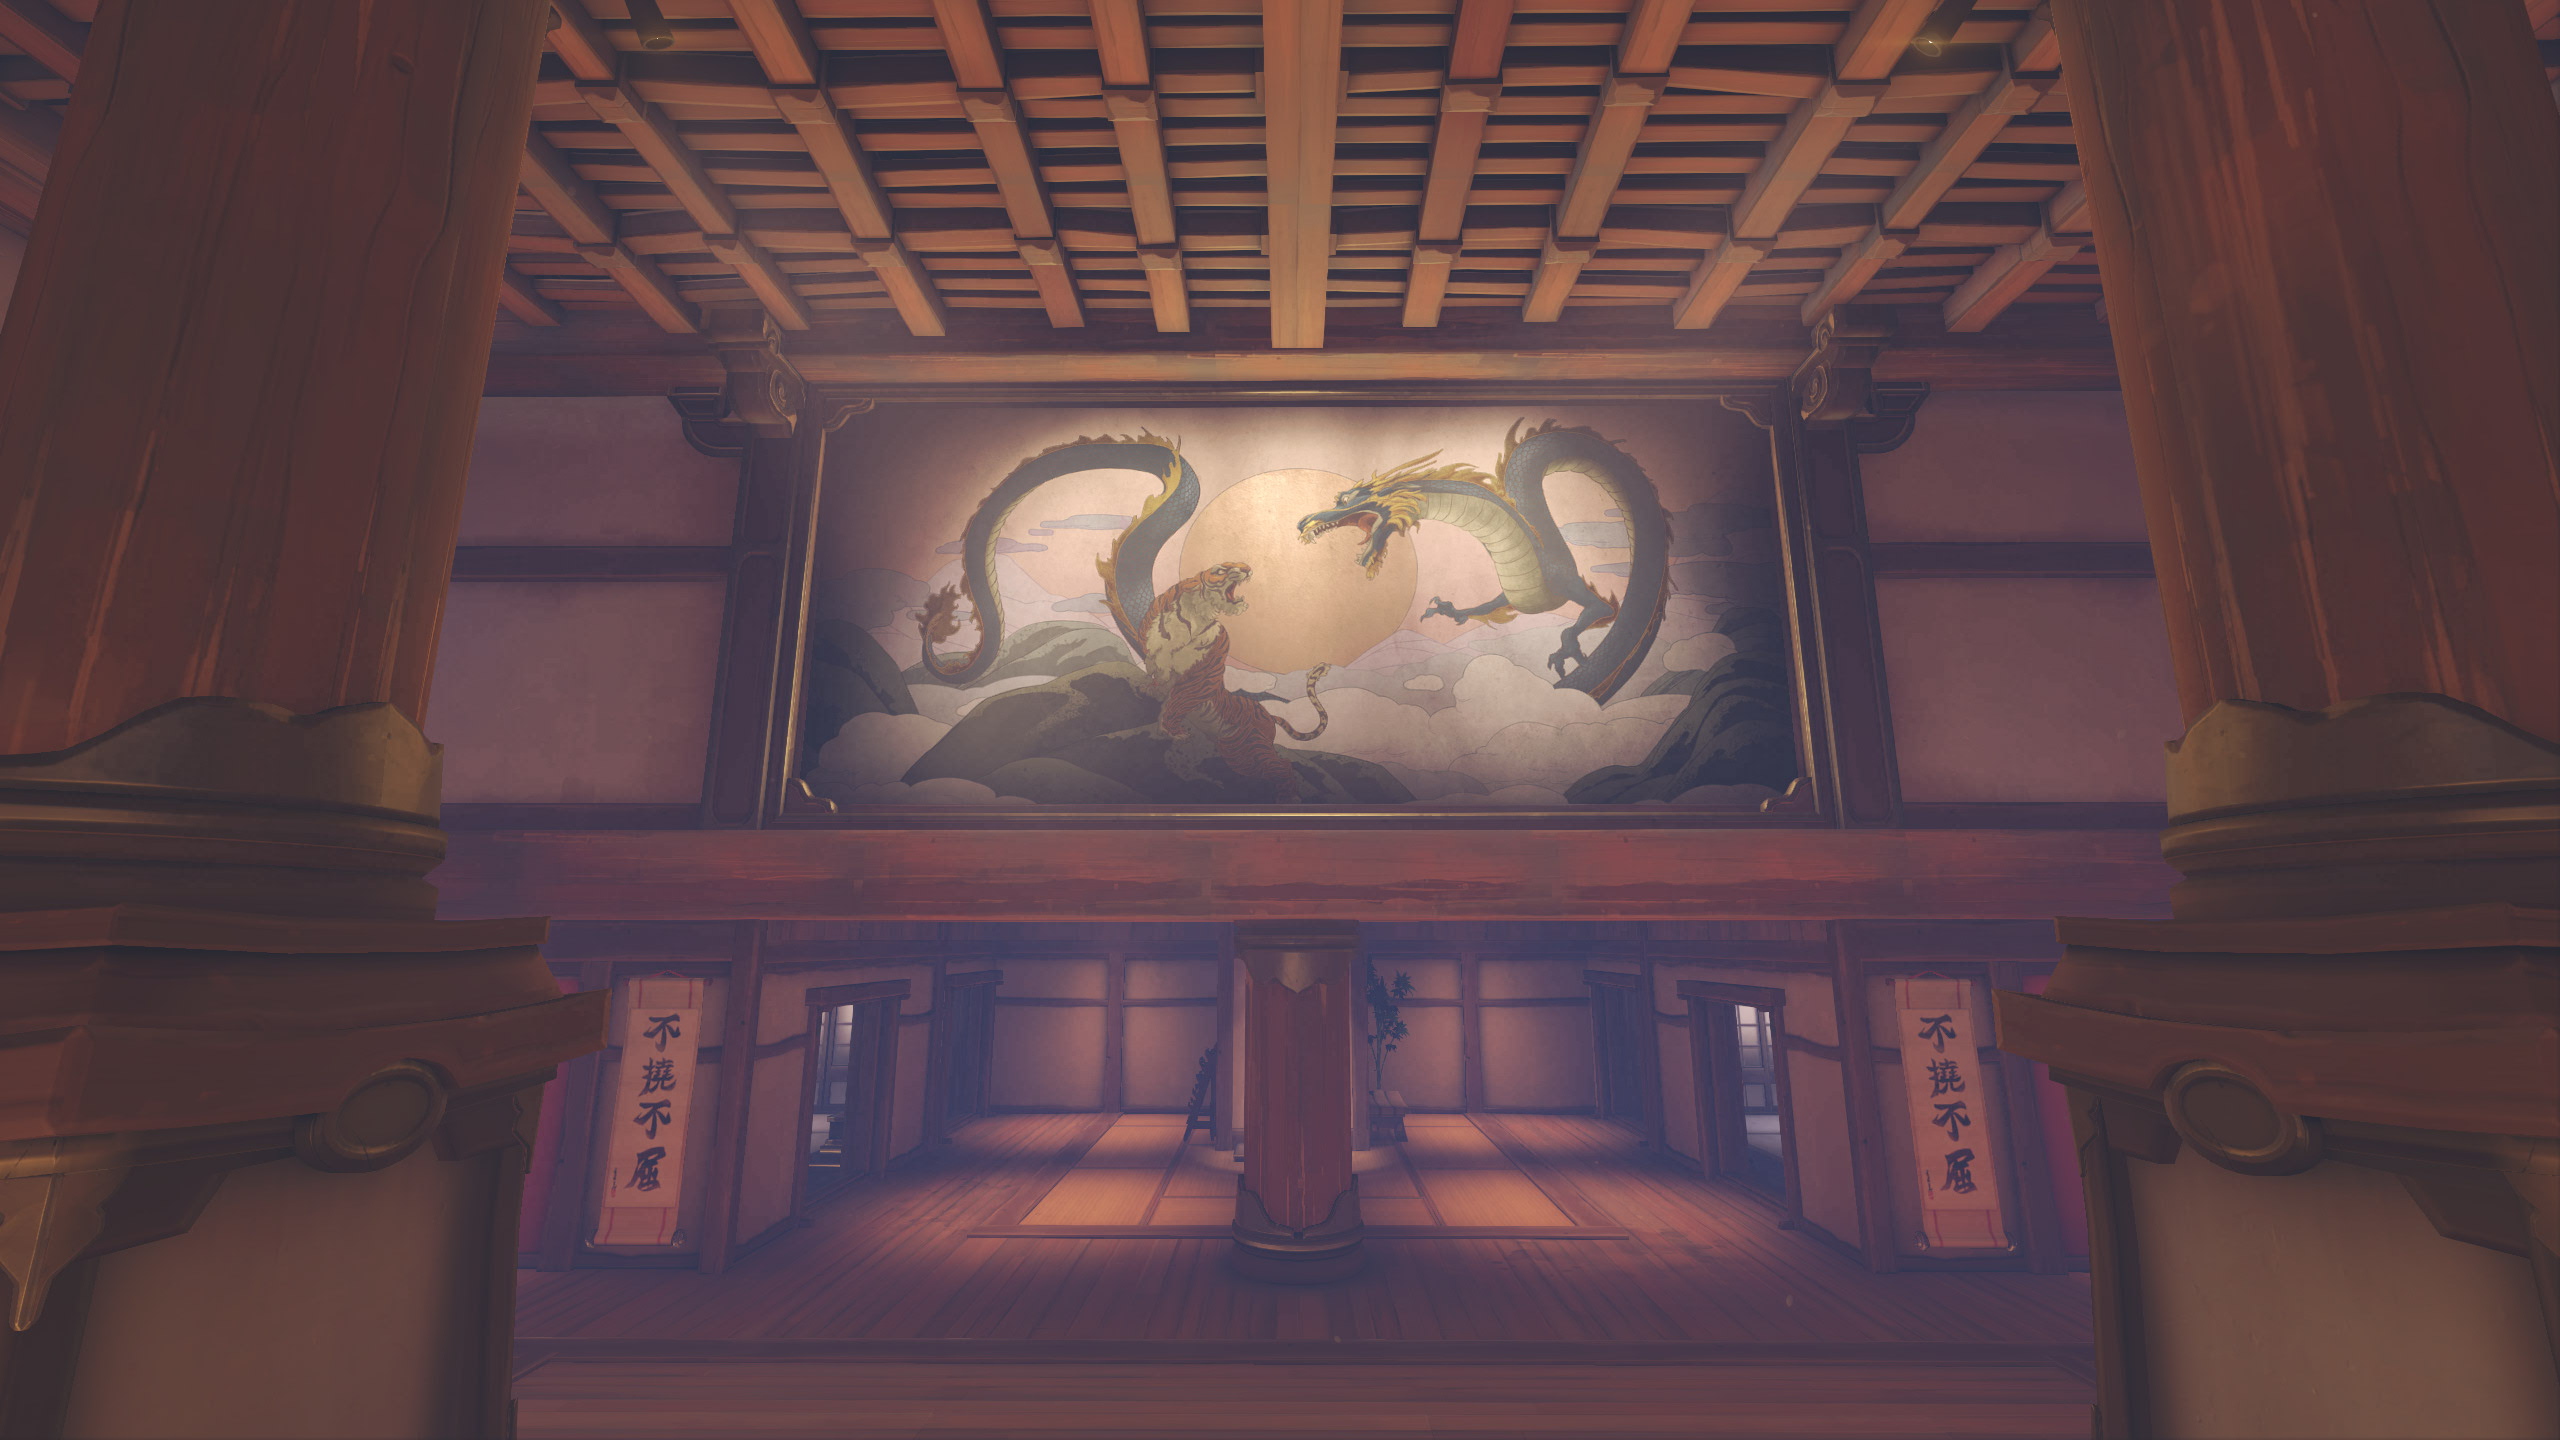
\includegraphics[width=0.22\textwidth]{images/test-image/synthetic-inside-04.jpg} &
    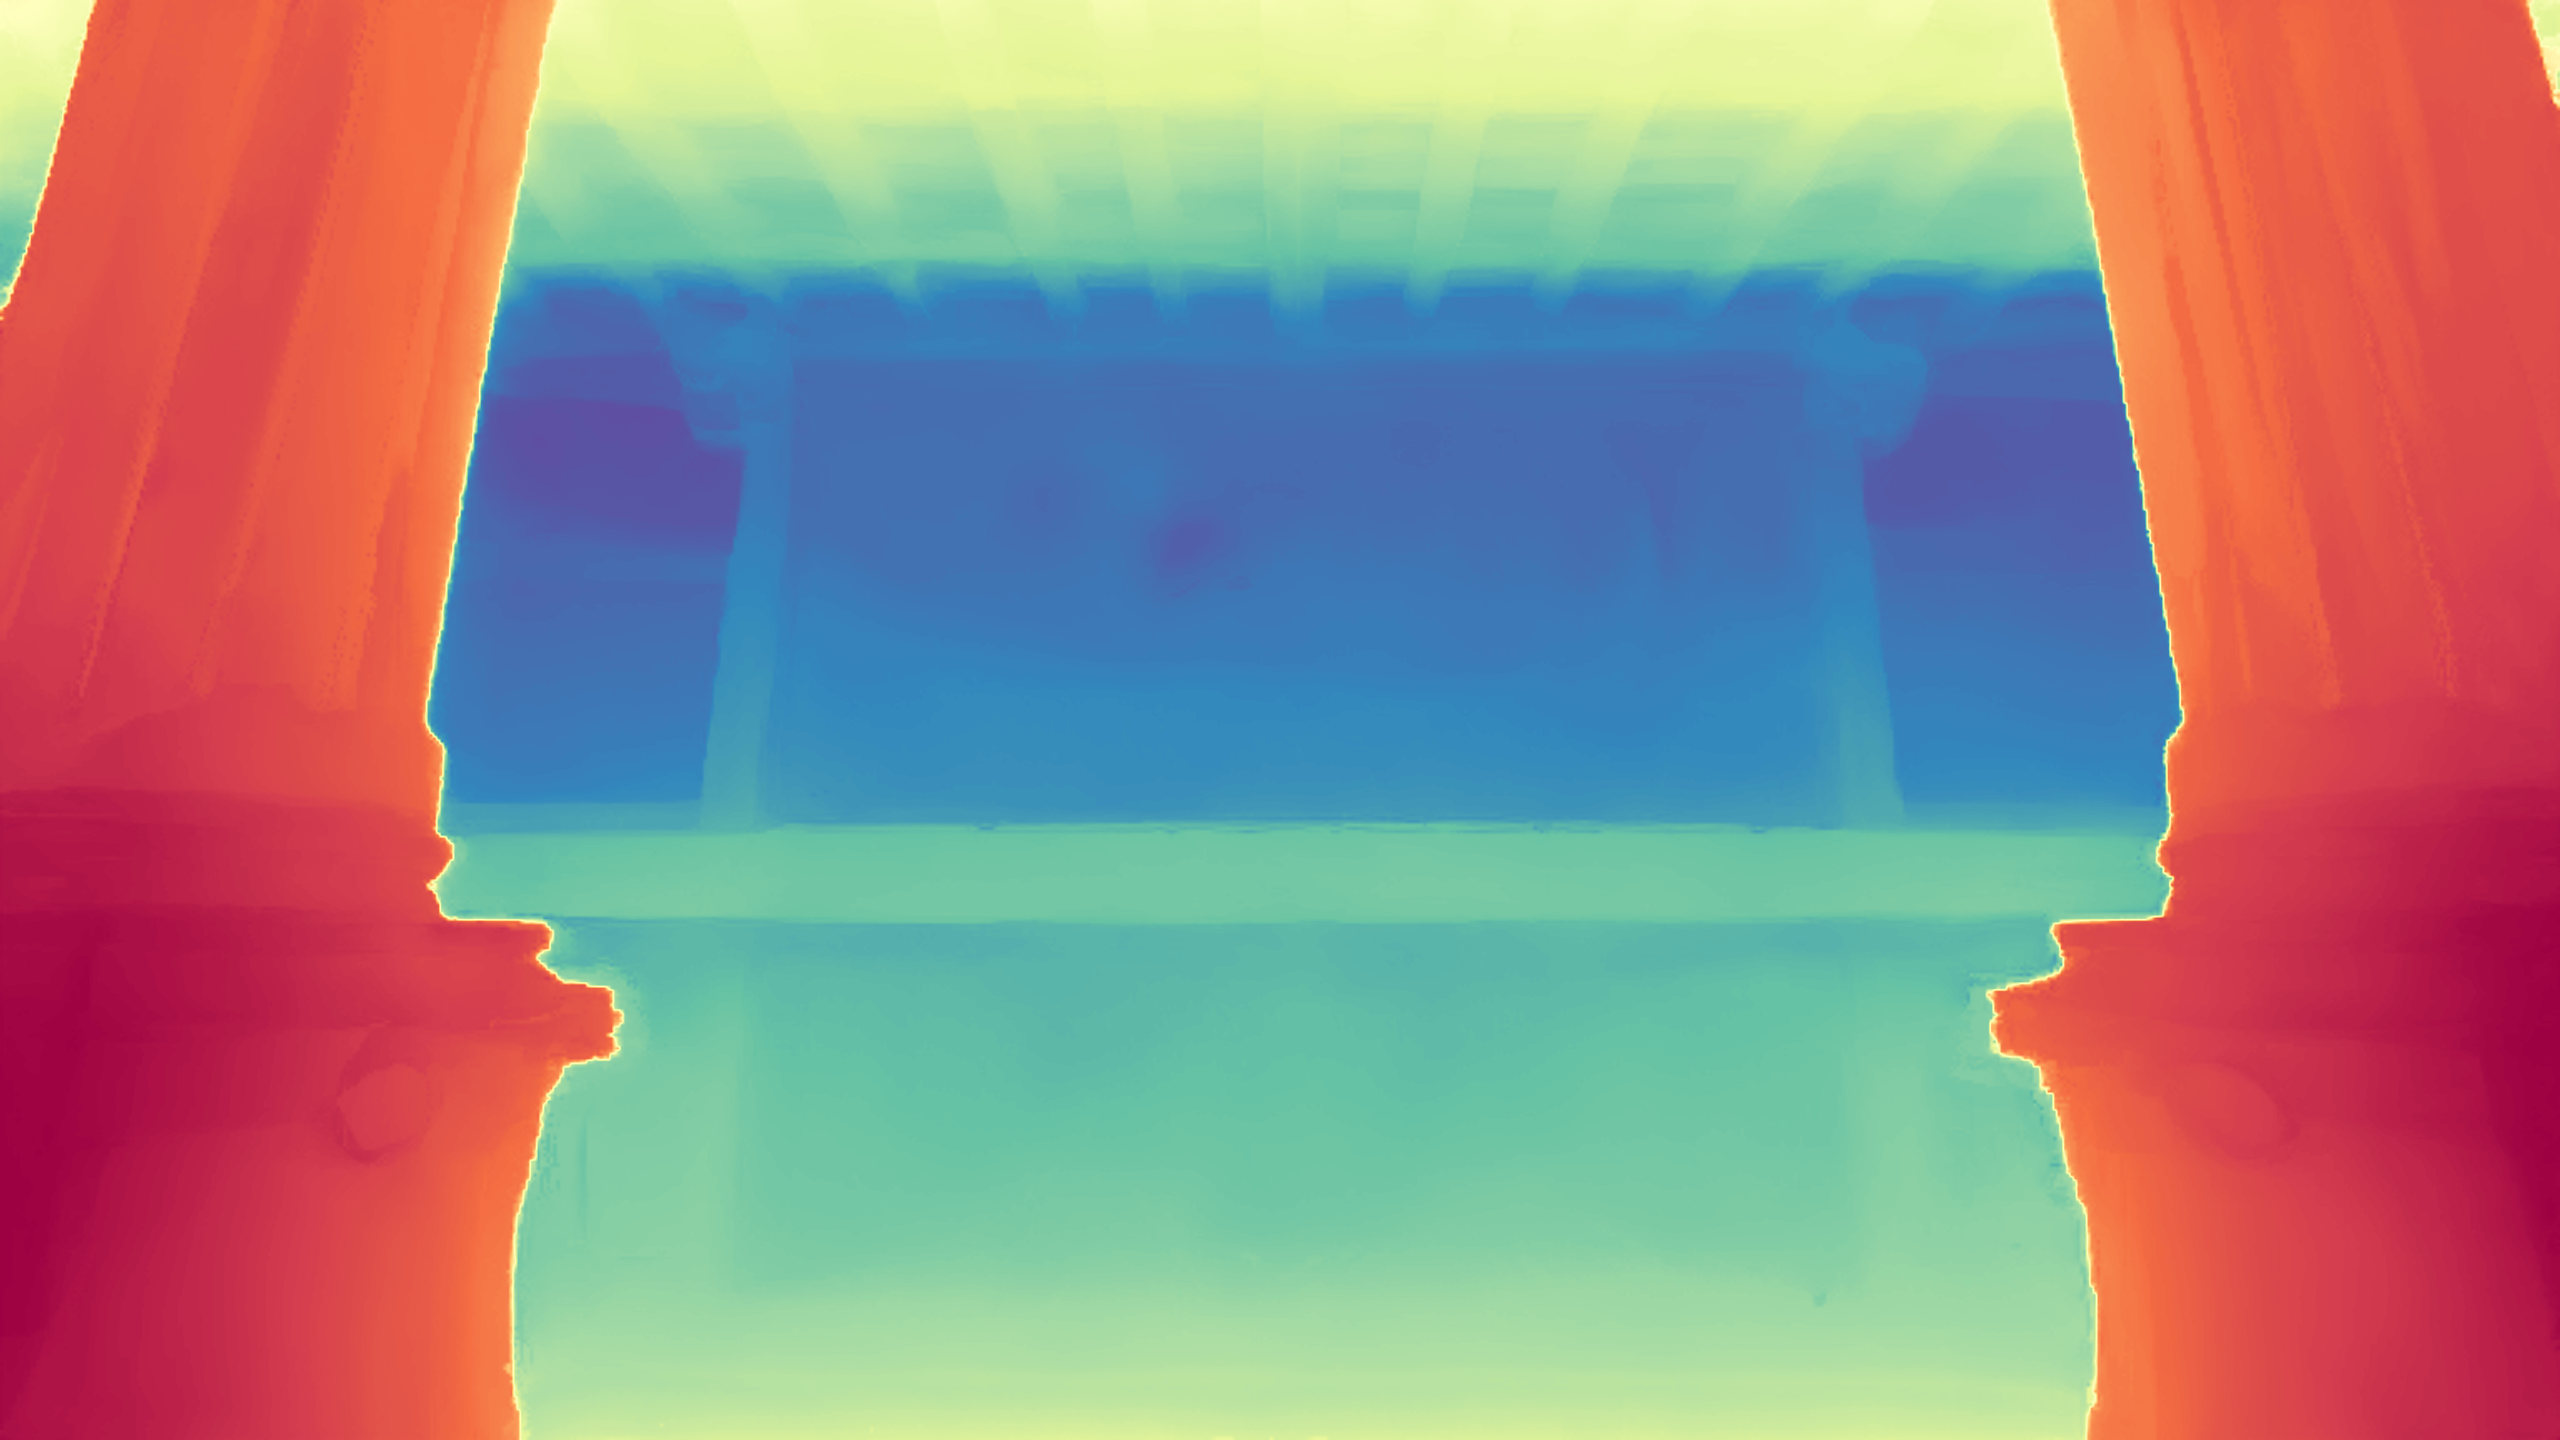
\includegraphics[width=0.22\textwidth]{images/trained/synthetic-inside-04_pred_colored.png} &
    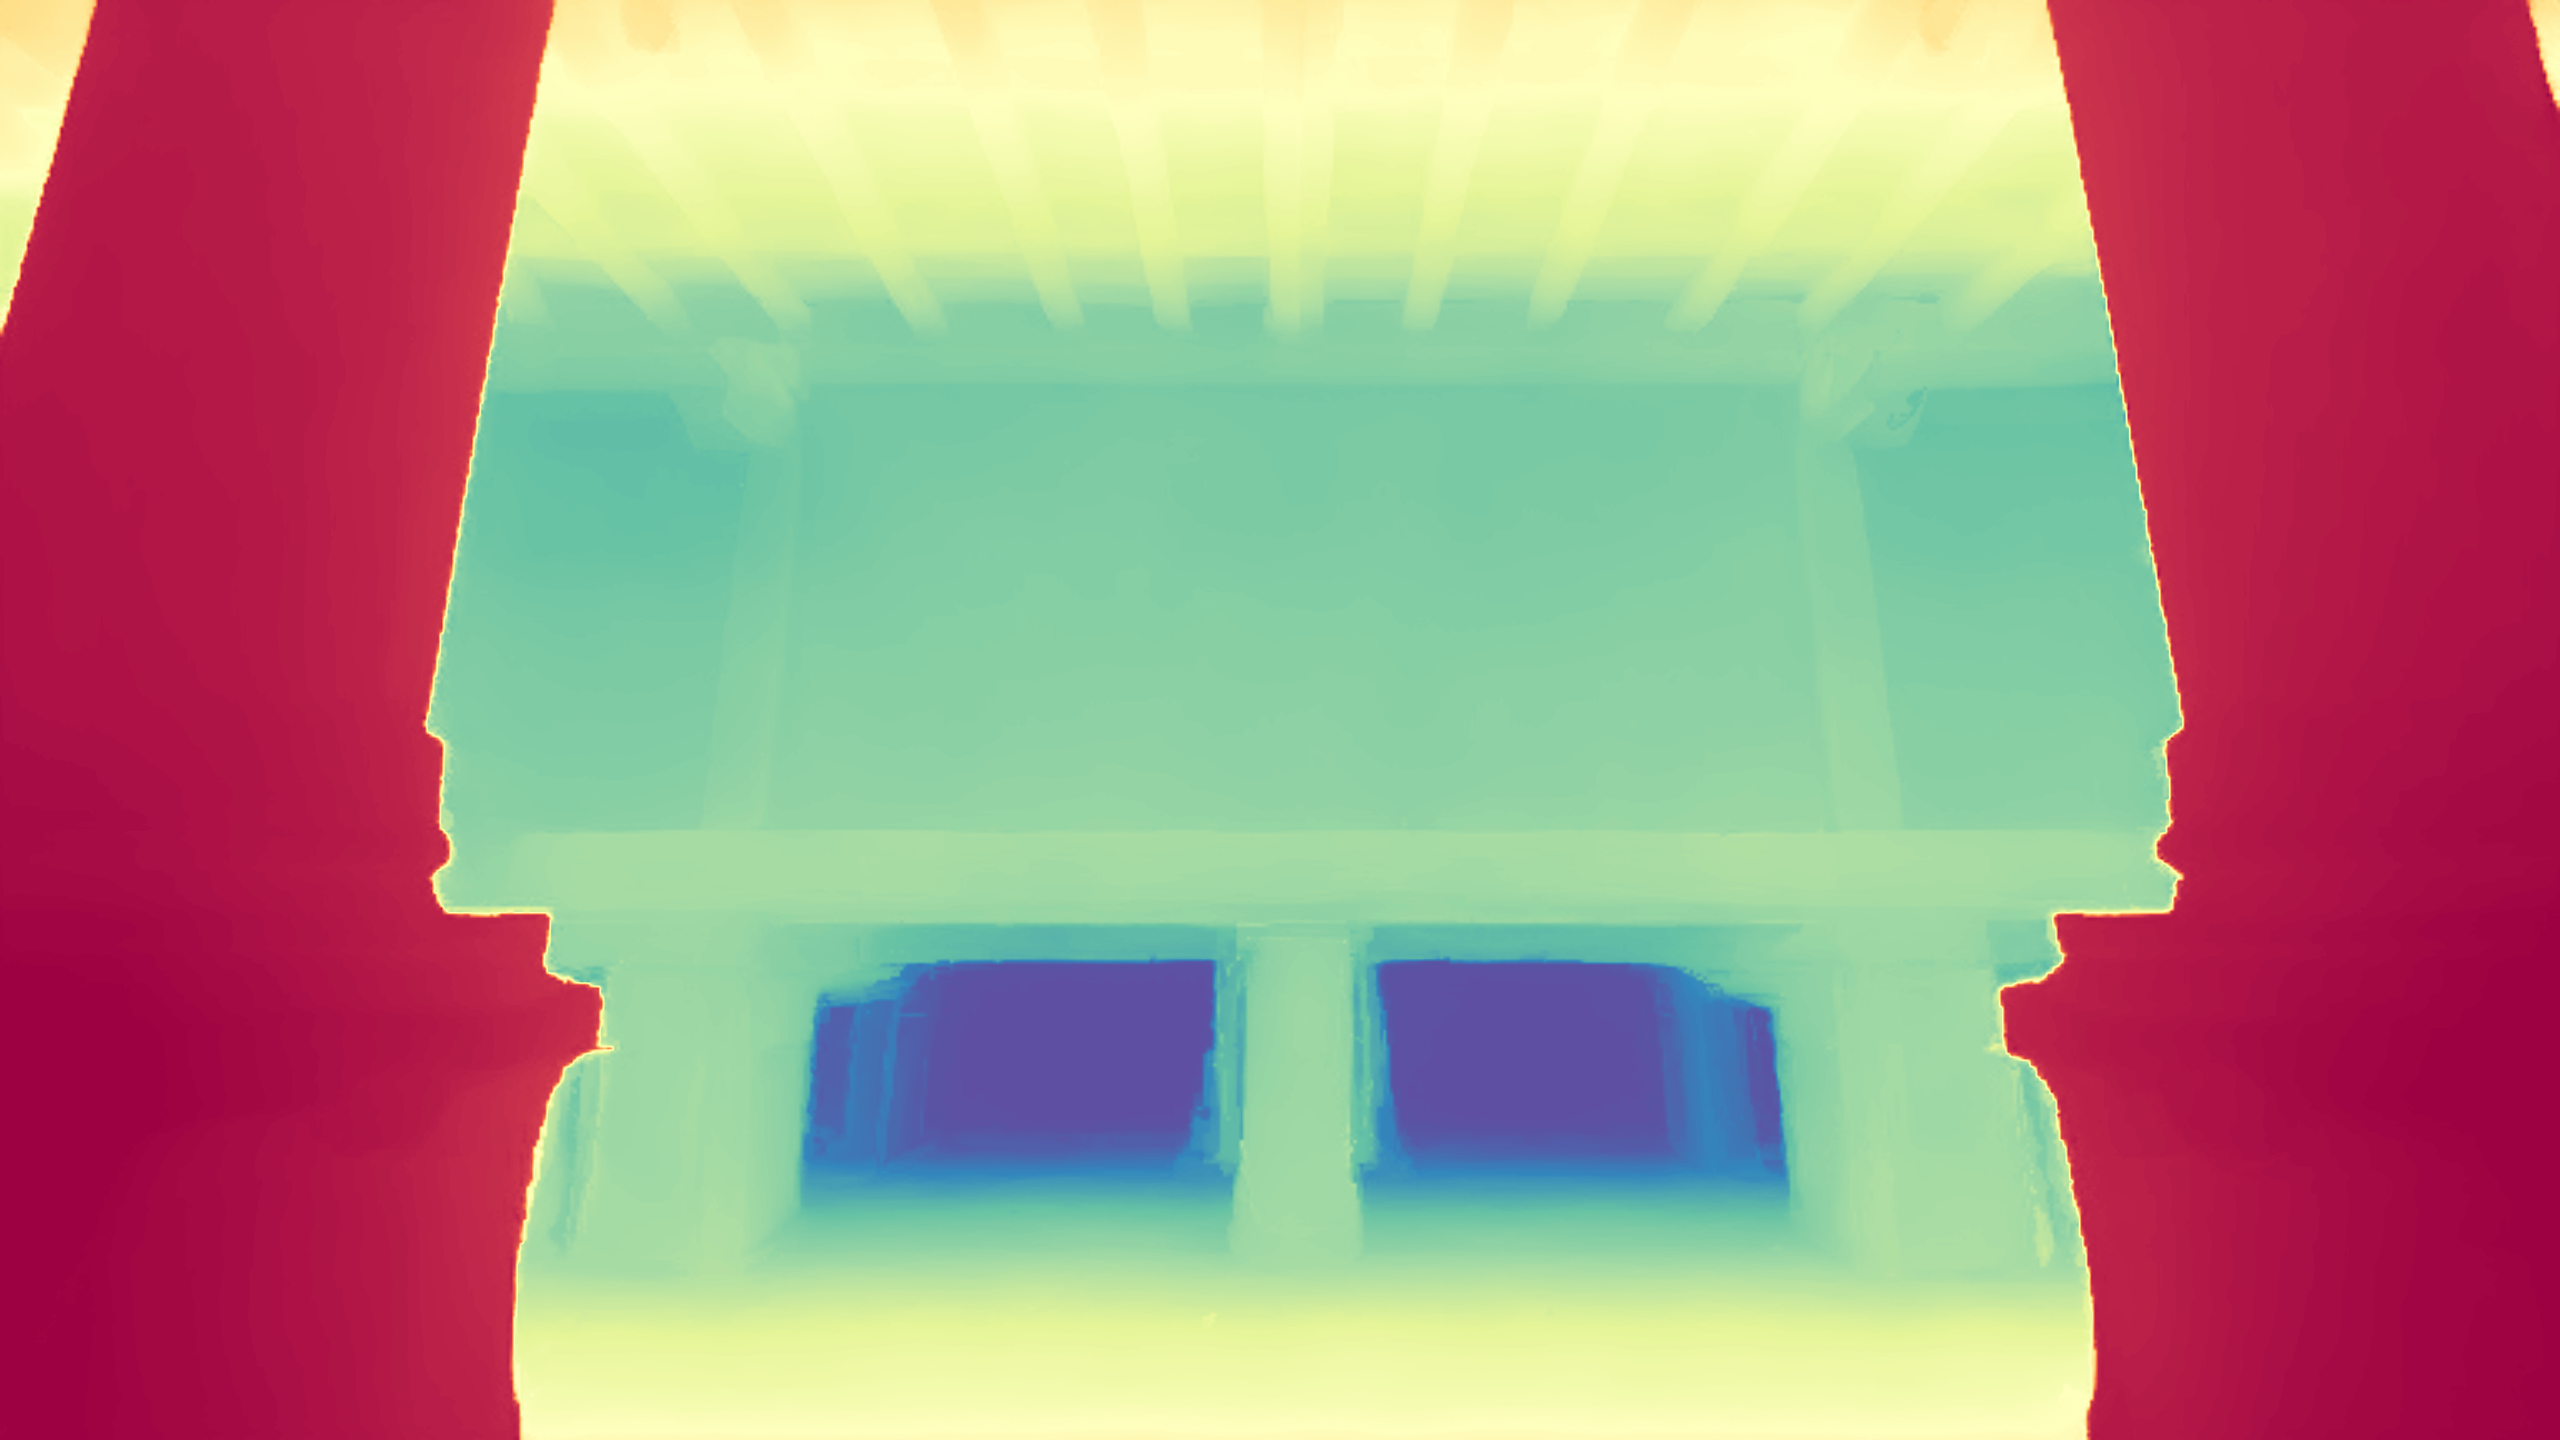
\includegraphics[width=0.22\textwidth]{images/pretrained/synthetic-inside-04_pred_colored.png} &
    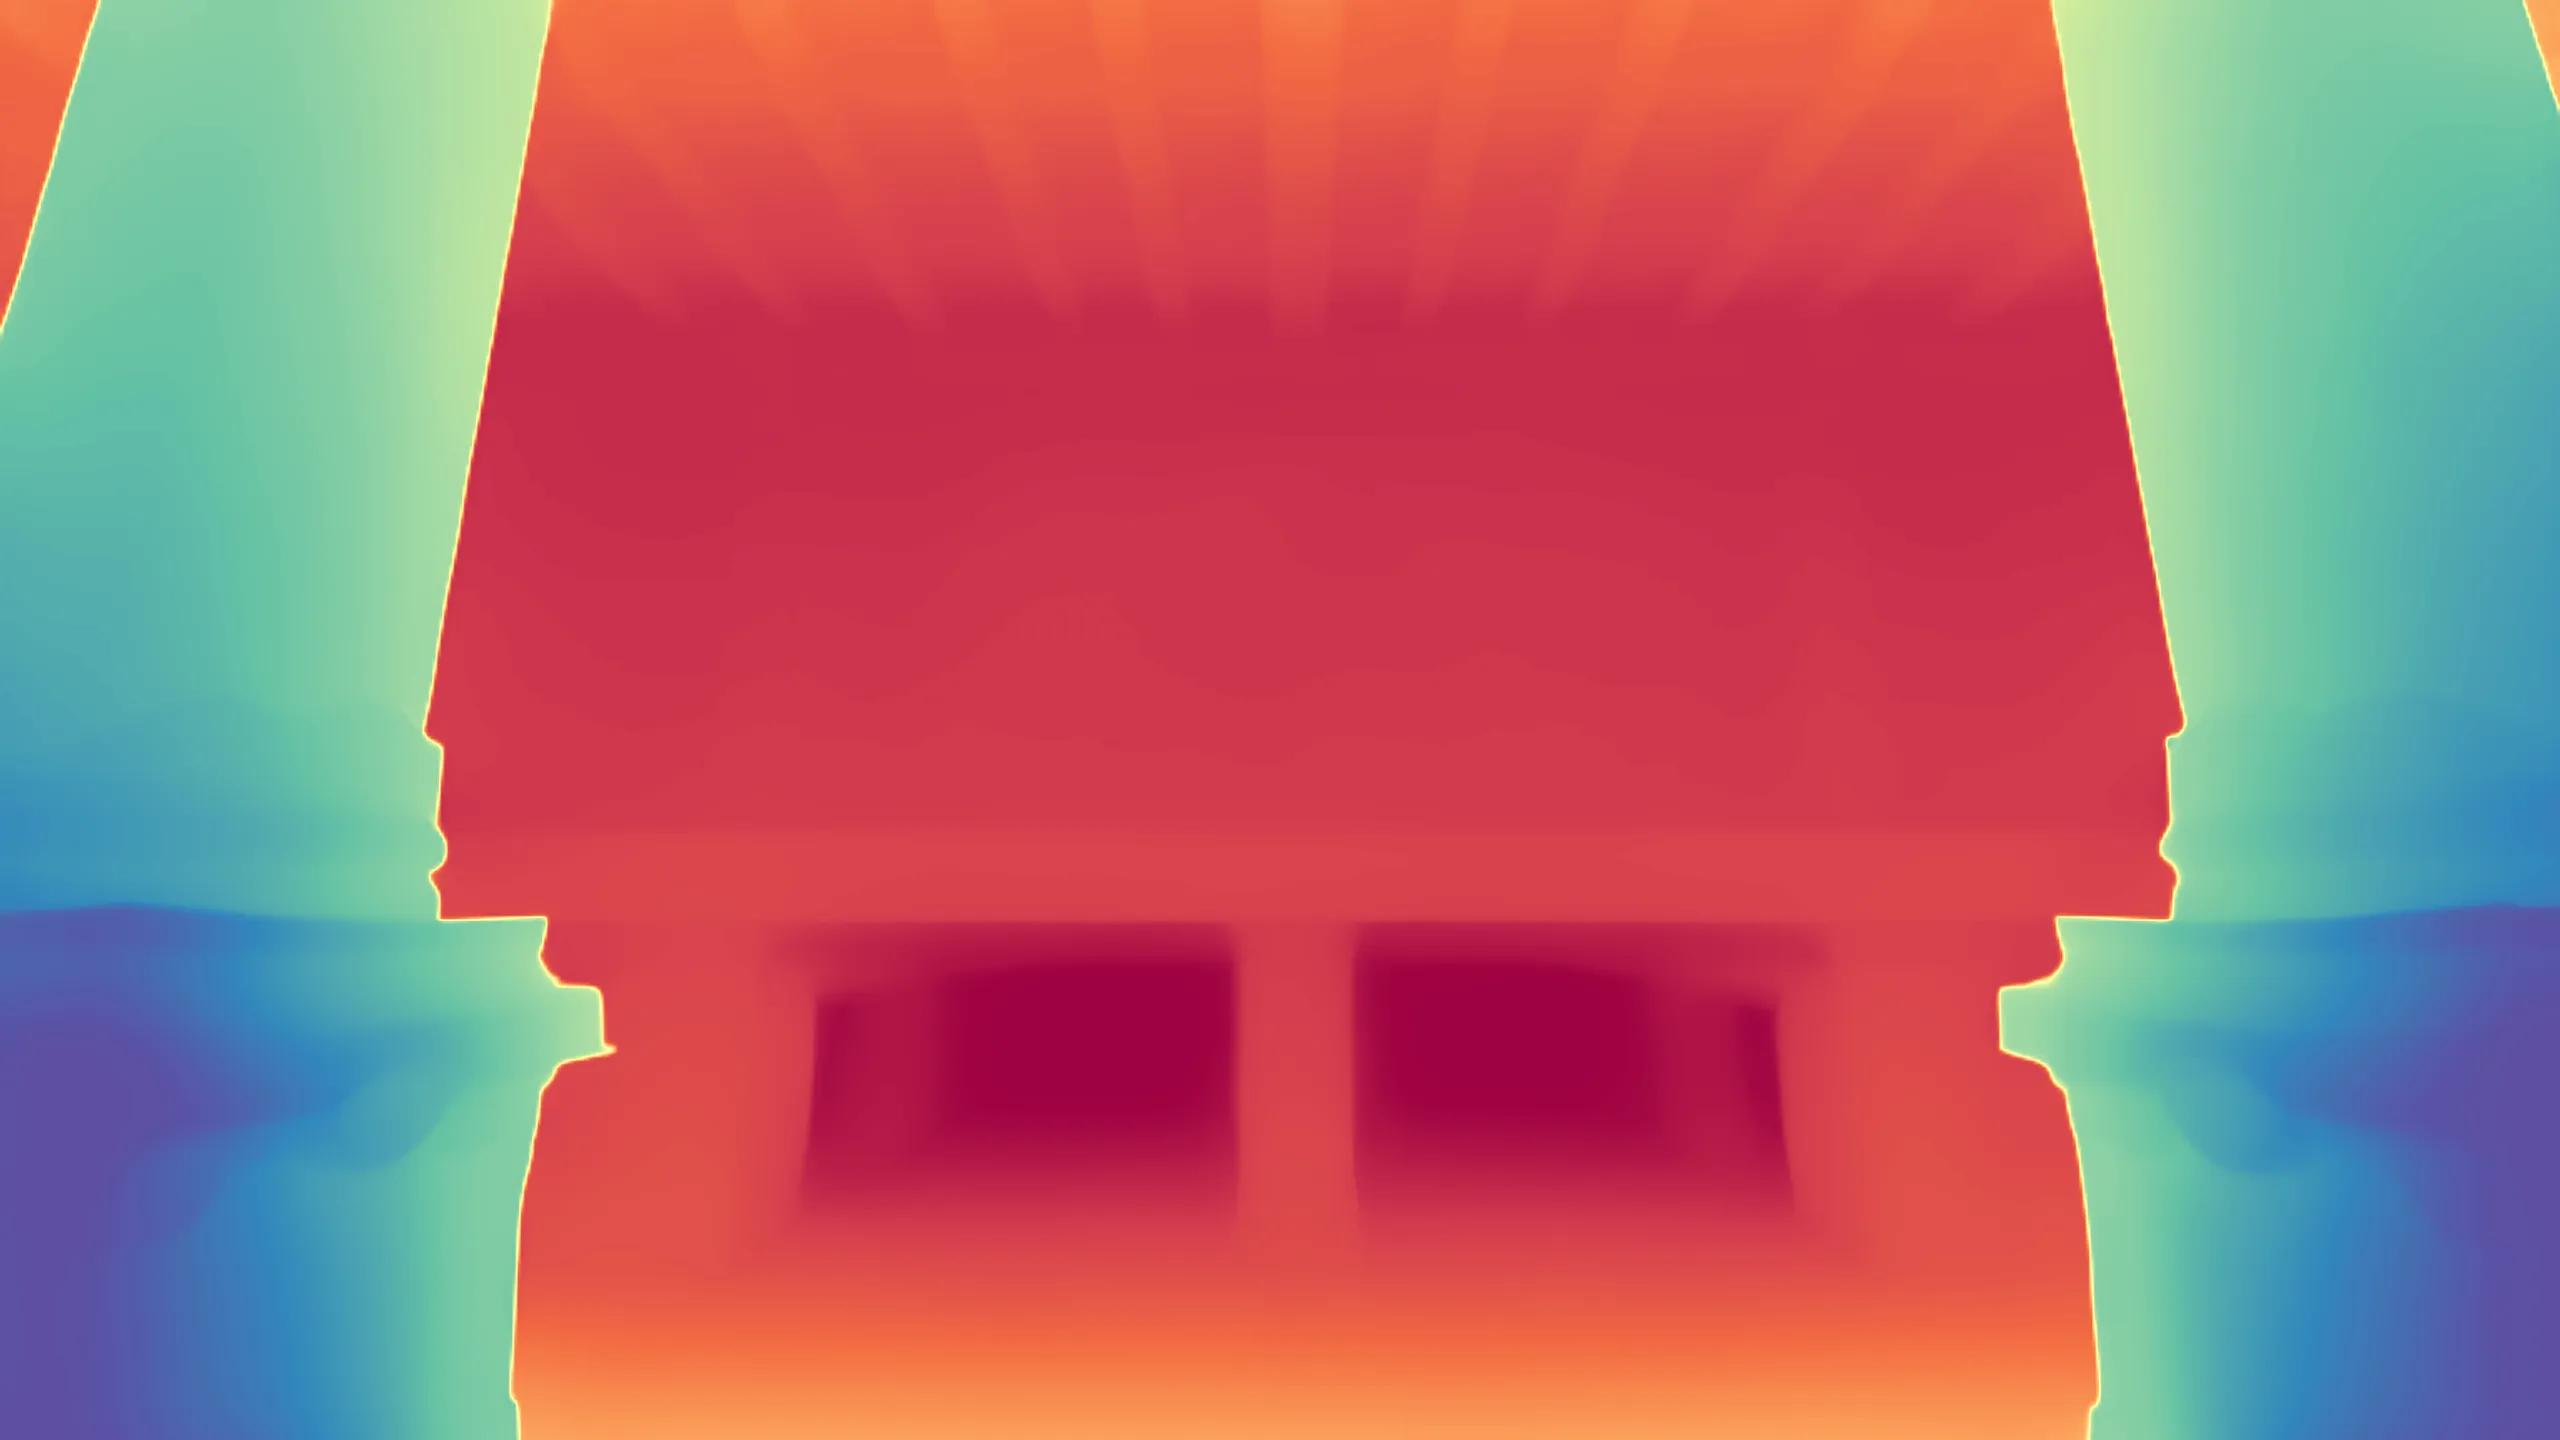
\includegraphics[width=0.22\textwidth]{images/depthmaster/synthetic-inside-04_pred_colored.jpg} \\

    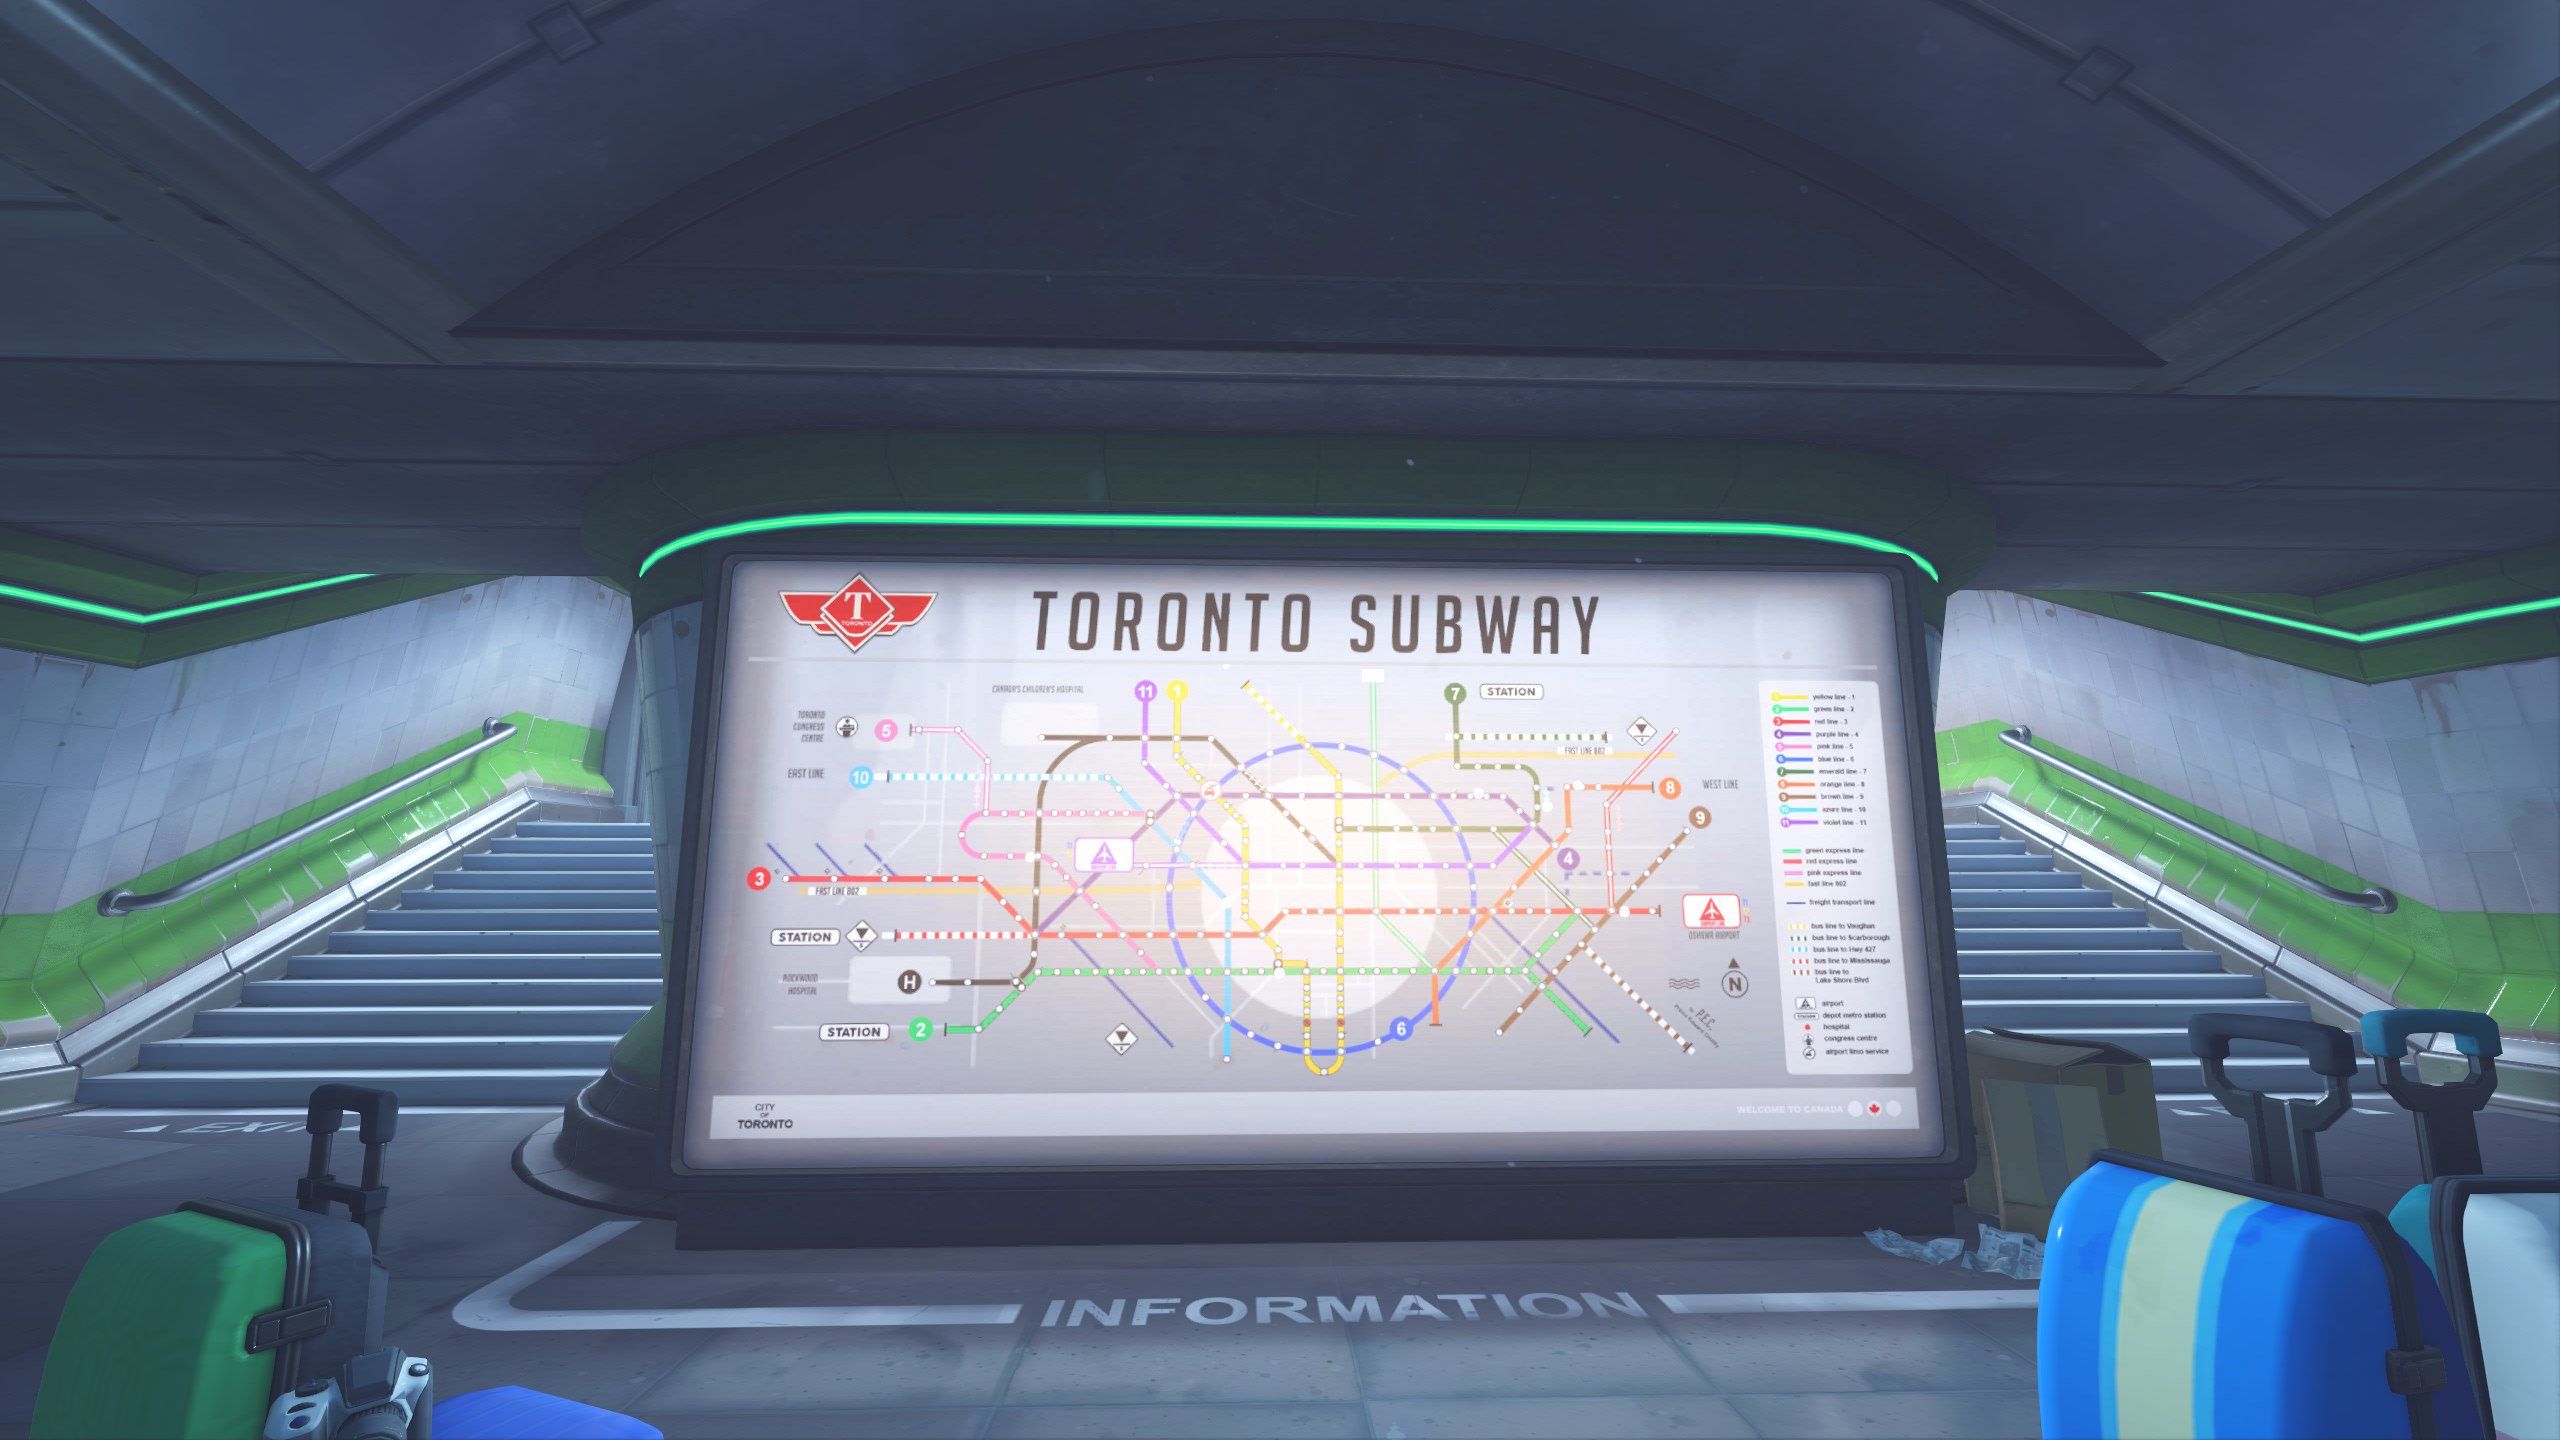
\includegraphics[width=0.22\textwidth]{images/test-image/synthetic-inside-05.jpg} &
    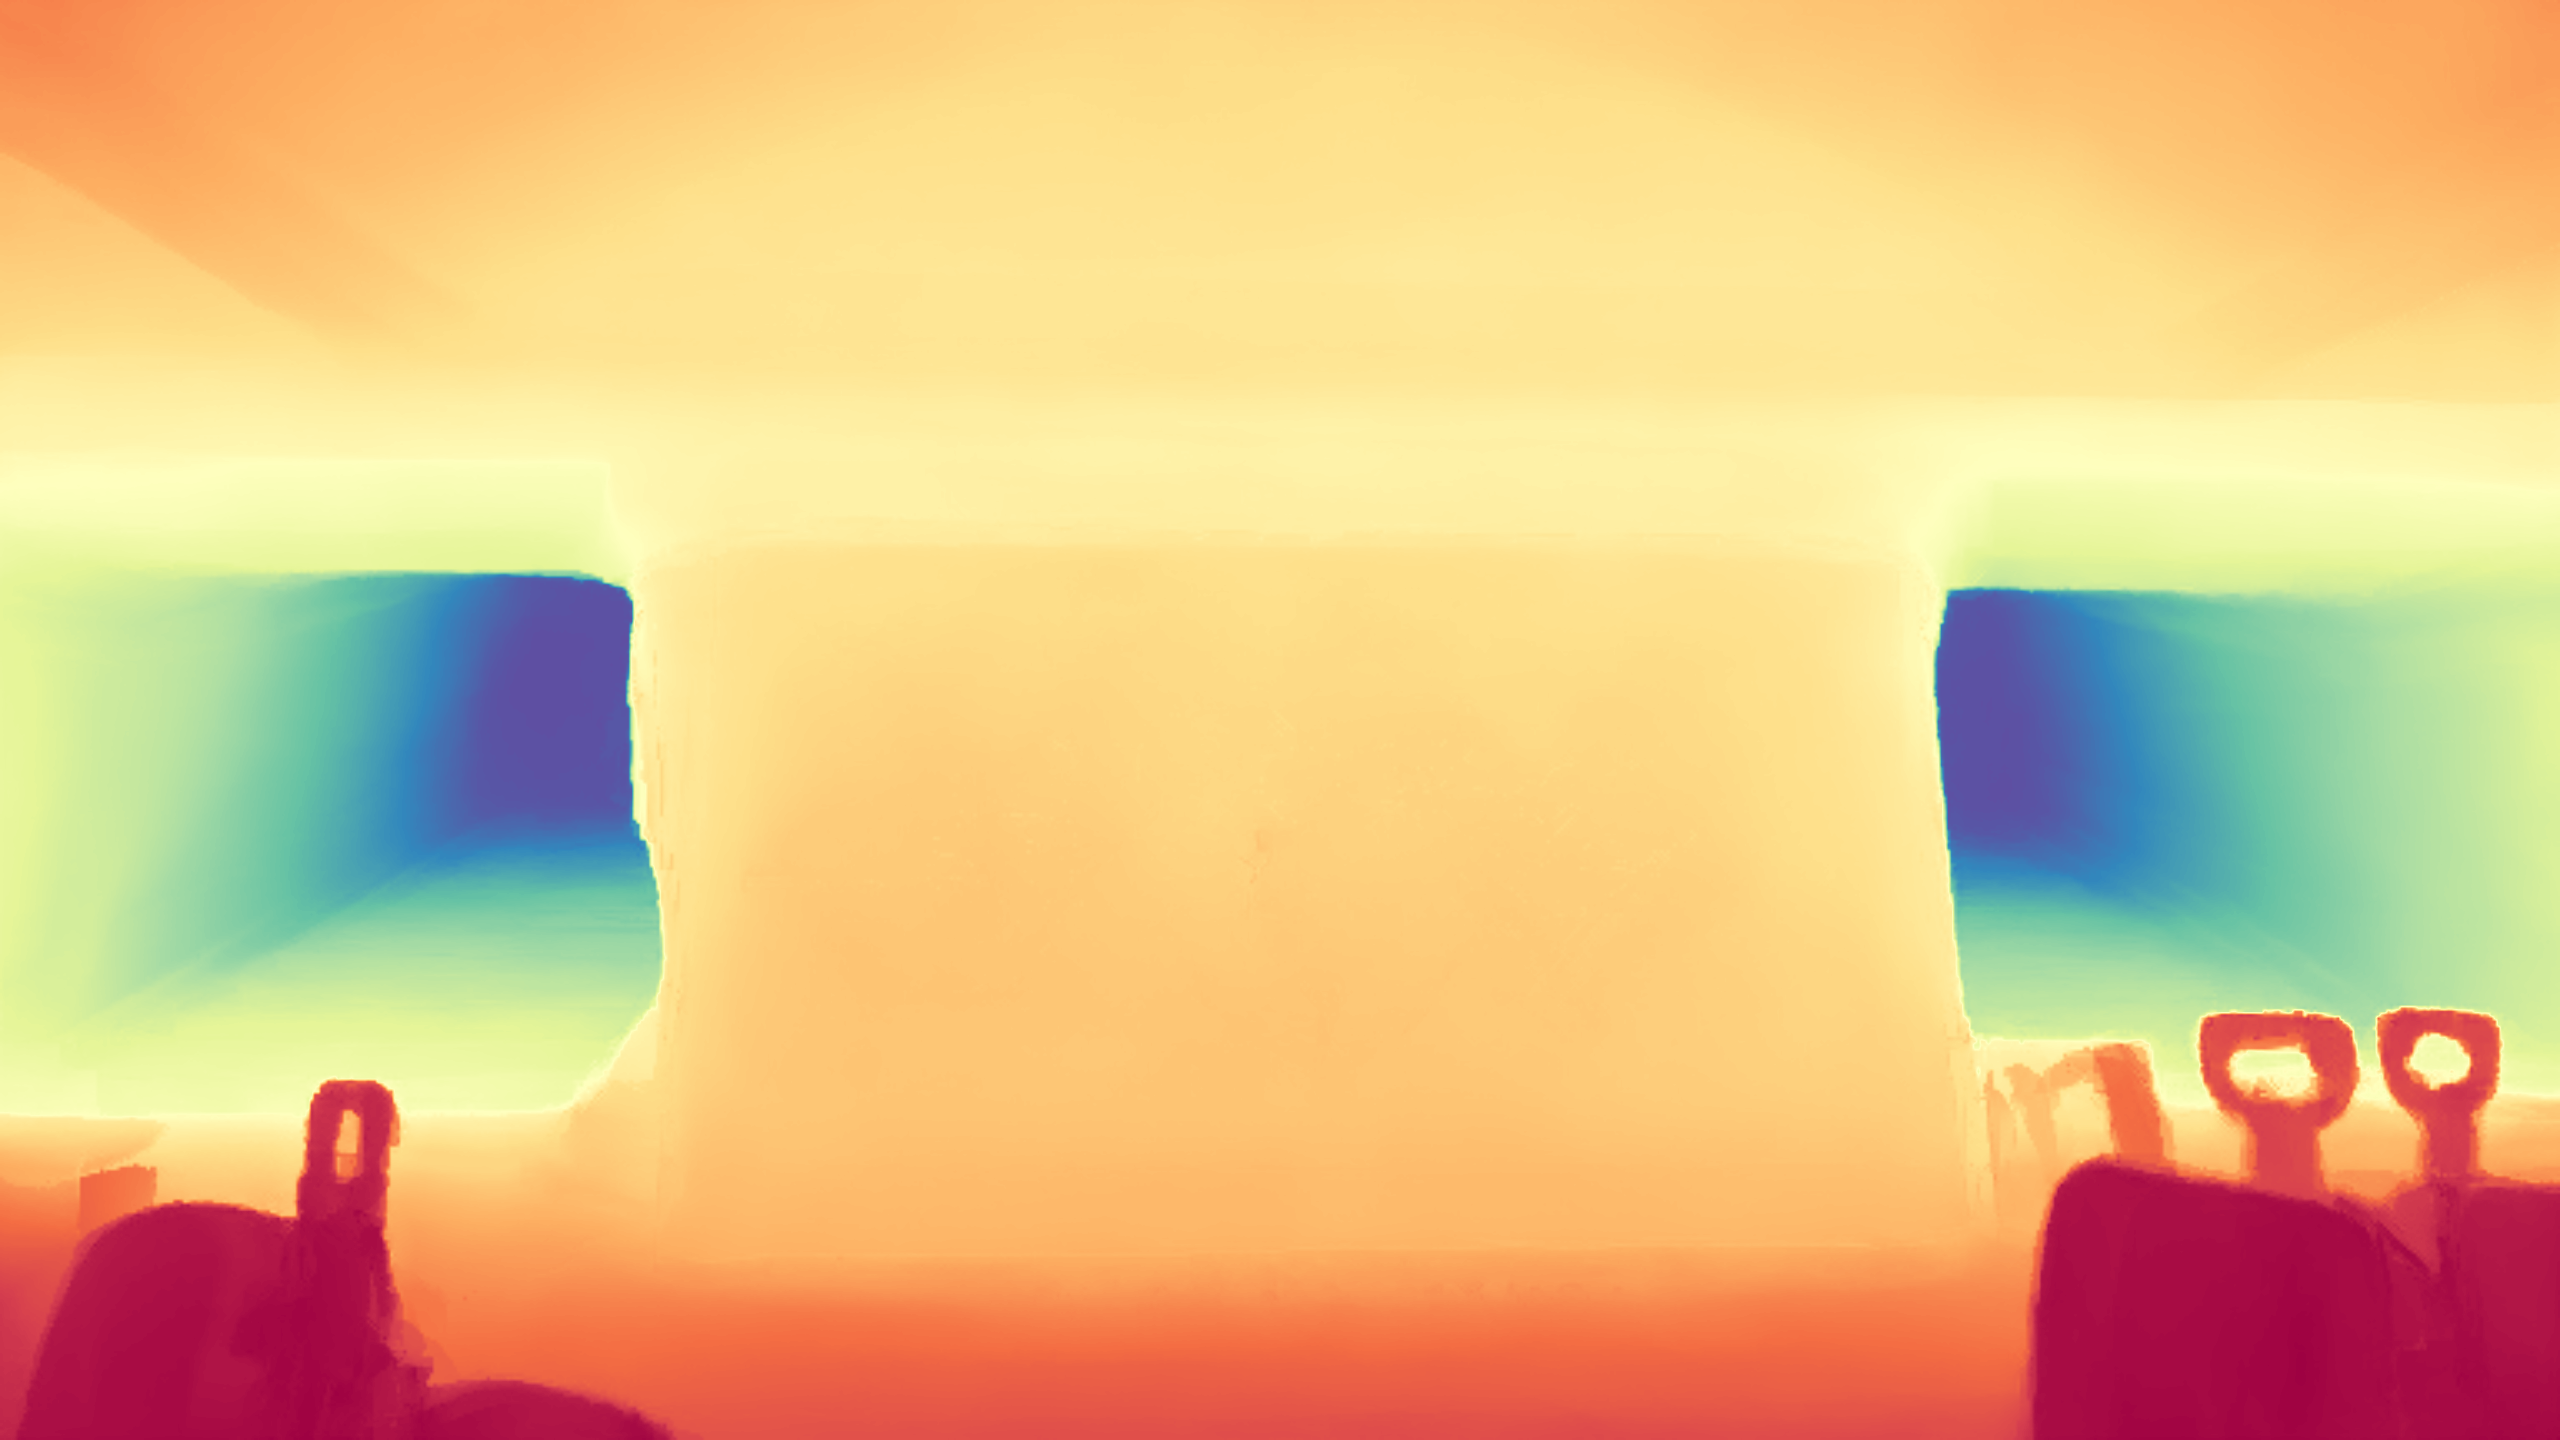
\includegraphics[width=0.22\textwidth]{images/trained/synthetic-inside-05_pred_colored.png} &
    \includegraphics[width=0.22\textwidth]{images/pretrained/synthetic-inside-05_pred_colored.png} &
    \includegraphics[width=0.22\textwidth]{images/depthmaster/synthetic-inside-05_pred_colored.jpg} \\

    \includegraphics[width=0.22\textwidth]{images/test-image/synthetic-outside-01.jpg} &
    \includegraphics[width=0.22\textwidth]{images/trained/synthetic-outside-01_pred_colored.png} &
    \includegraphics[width=0.22\textwidth]{images/pretrained/synthetic-outside-01_pred_colored.png} &
    \includegraphics[width=0.22\textwidth]{images/depthmaster/synthetic-outside-01_pred_colored.jpg} \\

    \includegraphics[width=0.22\textwidth]{images/test-image/synthetic-outside-02.jpg} &
    \includegraphics[width=0.22\textwidth]{images/trained/synthetic-outside-02_pred_colored.png} &
    \includegraphics[width=0.22\textwidth]{images/pretrained/synthetic-outside-02_pred_colored.png} &
    \includegraphics[width=0.22\textwidth]{images/depthmaster/synthetic-outside-02_pred_colored.jpg} \\

    \includegraphics[width=0.22\textwidth]{images/test-image/synthetic-outside-03.jpg} &
    \includegraphics[width=0.22\textwidth]{images/trained/synthetic-outside-03_pred_colored.png} &
    \includegraphics[width=0.22\textwidth]{images/pretrained/synthetic-outside-03_pred_colored.png} &
    \includegraphics[width=0.22\textwidth]{images/depthmaster/synthetic-outside-03_pred_colored.jpg} \\
  \end{tabular}
  \caption{续上表,除第一张图外,其余均为合成图像,包括室内、室外图像。}
\end{figure}

\newpage

\section{DepthMaster}

\textit{\textbf{DepthMaster}}是一个新的深度估计模型,同样是基于\textit{\textbf{Stable Diffusion}}的\textit{Depth2Img}模型进行微调,从而进行深度估计任务。

\begin{figure}[h!]
  \centering
  \includegraphics[width=0.8\textwidth]{images/wild_result_v1_notxt.png}
\end{figure}

\\

\textit{\textbf{DepthMaster}}的创新点主要在于它对\textit{\textbf{Stable Diffusion}}中U-net的编码器的修改,提出了一种两阶段的训练过程,从而实现了较好的深度估计效果。
目前\textit{\textbf{DepthMaster}}在nyudepthv2上的准确度排名为第7名(详见附录)。 \\
\textit{\textbf{DepthMaster}}的模型示意图如下:

\begin{figure}[h!]
  \centering
  \includegraphics[width=0.9\textwidth]{images/framework_v6.png}
  \caption{We propose DepthMaster, a approach that customizes generative features in diffusion models to suit the discriminative depth estimation task. We introduce a Feature Alignment module to mitigate overfitting to texture details with high-quality external features and a Fourier Enhancement module to refine fine-grained details in the frequency domain.}
\end{figure}


\newpage

\section{Appendix}

\begin{table}[h!]
    \centering
    \small
    \label{tab:depth_models}
    \begin{tabular}{l l c c c c c c}
        \toprule
        Rank & Model & Abs Rel & RMSE & log 10 & Delta_1 & Delta_2 & Delta_3 \\
        \midrule
        1 & HybridDepth & 0.026 & 0.128 & & 0.988 & 1.000 & 1.000 \\
        2 & Distill Any Depth & 0.043 & & & 0.981 & & \\
        3 & UniK3D (FT, metric) & 0.044 & 0.173 & 0.019 & 0.989 & 0.998 & 1.000 \\
        4 & UniDepthV2 (FT, metric) & 0.046 & 0.180 & 0.020 & 0.988 & 0.998 & 1.000 \\
        5 & PrimeDepth + Depth Anything & 0.046 & & & 0.977 & & \\
        6 & Metric3Dv2 (L, FT) & 0.047 & 0.183 & 0.020 & 0.989 & 0.998 & 1.000 \\
        7 & DepthMaster & 0.050 & & & 0.972 & & \\
        8 & GRIN & 0.051 & 0.251 & & & & \\
        9 & Marigold + E2E FT (zero-shot) & 0.052 & & & 0.966 & & \\
        10 & Marigold & 0.055 & 0.224 & 0.024 & 0.964 & 0.991 & 0.998 \\
        \bottomrule
    \end{tabular}
    \caption{Performance Metrics of Various Depth Estimation Models}
\end{table}

\begin{table}[h!]
    \centering
    \label{tab:metrics_explanation}
    \begin{tabular}{lp{8cm}}
        \toprule
        \textbf{指标} & \textbf{含义} \\
        \midrule
        Abs Rel (Absolute Relative Error) & 绝对相对误差:$\frac{1}{N}\sum_{i=1}^N \frac{|y_i - \hat{y}_i|}{y_i}$ \\
        & 预测深度值与真实深度值的绝对相对差异,值越小越好 \\[0.5em]
        
        RMSE (Root Mean Square Error) & 均方根误差:$\sqrt{\frac{1}{N}\sum_{i=1}^N (y_i - \hat{y}_i)^2}$ \\
        & 预测值与真实值的标准差,对大误差更敏感,值越小越好 \\[0.5em]
        
        log10 & 对数误差:$\frac{1}{N}\sum_{i=1}^N |\log_{10} y_i - \log_{10} \hat{y}_i|$ \\
        & 深度值的对数空间误差,值越小越好 \\[0.5em]
        
        Delta\_1 ($\delta_1$) & 阈值准确率:$\% \text{ of } y_i \text{ s.t. } \max(\frac{y_i}{\hat{y}_i}, \frac{\hat{y}_i}{y_i}) < 1.25$ \\
        & 预测值与真实值比率在1.25以内的百分比,值越大越好 \\[0.5em]
        
        Delta\_2 ($\delta_2$) & 阈值准确率:比率在$1.25^2$ (≈1.56)以内的百分比 \\
        & 更宽松的准确率评估,值越大越好 \\[0.5em]
        
        Delta\_3 ($\delta_3$) & 阈值准确率:比率在$1.25^3$ (≈1.95)以内的百分比 \\
        & 最宽松的准确率评估,值越大越好 \\
        \bottomrule
    \end{tabular}
    \caption{深度估计评估指标说明}
\end{table}

\end{document}